%%%%%%%%%%%%%%%%%%%%%%%%%%%%%%%%%%%%%%%%%%%%%%%%%%%%%%%%%%%%%%%%%%%%%%%%
%% Adaptação do projeto UECETeX2 para uso acadêmico no IFSP 	      %%
%%                                                                    %%
%% Customizações do abnTeX2 (http://abnTeX2.googlecode.com)           %%
%% para a Universidade Estadual do Ceara - UECE                       %%
%%                                                                    %%
%% This work may be distributed and/or modified under the             %% 
%% conditions of the LaTeX Project Public License, either version 1.3 %%
%% of this license or (at your option) any later version.             %%
%% The latest version of this license is in                           %%
%%   http://www.latex-project.org/lppl.txt                            %%
%% and version 1.3 or later is part of all distributions of LaTeX     %%
%% version 2005/12/01 or later.                                       %%
%%                                                                    %%
%% This work has the LPPL maintenance status `maintained'.            %%
%%                                                                    %%
%% The Current Maintainer of this work is Thiago Nascimento           %%
%%                                                                    %%
%% Project available on: https://github.com/thiagodnf/uecetex2        %%
%%                                                                    %%
%% Further information about abnTeX2                                  %%
%% are available on http://abntex2.googlecode.com/                    %%
%%                                                                    %%
%%%%%%%%%%%%%%%%%%%%%%%%%%%%%%%%%%%%%%%%%%%%%%%%%%%%%%%%%%%%%%%%%%%%%%%%

%%%%%%%%%%%%%%%%%%%%%%%%%%%%%%%%%%%%%%%%%%%%%%%%%%%%%%%%%%%%%%%%%%%%%%%%
%% Customizações do abnTeX2 (http://abnTeX2.googlecode.com)           %%
%% para a Universidade Estadual do Ceara - UECE                       %%
%%                                                                    %%
%% This work may be distributed and/or modified under the             %% 
%% conditions of the LaTeX Project Public License, either version 1.3 %%
%% of this license or (at your option) any later version.             %%
%% The latest version of this license is in                           %%
%%   http://www.latex-project.org/lppl.txt                            %%
%% and version 1.3 or later is part of all distributions of LaTeX     %%
%% version 2005/12/01 or later.                                       %%
%%                                                                    %%
%% This work has the LPPL maintenance status `maintained'.            %%
%%                                                                    %%
%% The Current Maintainer of this work is Thiago Nascimento           %%
%%                                                                    %%
%% Project available on: https://github.com/thiagodnf/uecetex2        %%
%%                                                                    %%
%% Further information about abnTeX2                                  %%
%% are available on http://abntex2.googlecode.com/                    %%
%%                                                                    %%
%%%%%%%%%%%%%%%%%%%%%%%%%%%%%%%%%%%%%%%%%%%%%%%%%%%%%%%%%%%%%%%%%%%%%%%%

\documentclass[        
    a4paper,          % Tamanho da folha A4
    12pt,             % Tamanho da fonte 12pt
    chapter=TITLE,    % Todos os capitulos devem ter caixa alta
    section=TITLE,    % Todas as secoes devem ter caixa alta
    oneside,          % Usada para impressao em apenas uma face do papel
    english,          % Hifenizacoes em ingles
    spanish,          % Hifenizacoes em espanhol
    brazil,            % Ultimo idioma eh o idioma padrao do documento
    hyphens        % Forçar a quebra de URLs que excedem a margem
]{abntex2}

% Importações de pacotes
\usepackage[utf8]{inputenc}                         % Acentuação direta
\usepackage[T1]{fontenc}                            % Codificação da fonte em 8 bits
\usepackage{graphicx}                               % Inserir figuras
\usepackage{amsfonts, amssymb, amsmath}             % Fonte e símbolos matemáticos
\usepackage{booktabs}                               % Comandos para tabelas
\usepackage{verbatim}                               % Texto é interpretado como escrito no documento
\usepackage{multirow, array}                        % Múltiplas linhas e colunas em tabelas
\usepackage{indentfirst}                            % Endenta o primeiro parágrafo de cada seção.
\usepackage{listings}                               % Utilizar codigo fonte no documento
\usepackage{xcolor}
\usepackage{microtype}                              % Para melhorias de justificação?
\usepackage[portuguese,ruled,lined]{algorithm2e}    % Escrever algoritmos
\usepackage{algorithmic}                            % Criar Algoritmos  
%\usepackage{float}                                  % Utilizado para criação de floats
\usepackage{amsgen}
\usepackage{lipsum}                                 % Usar a simulação de texto Lorem Ipsum
%\usepackage{titlesec}                               % Permite alterar os títulos do documento
\usepackage{tocloft}                                % Permite alterar a formatação do Sumário
\usepackage{etoolbox}                               % Usado para alterar a fonte da Section no Sumário
\usepackage[nogroupskip,nonumberlist,acronym]{glossaries}                % Permite fazer o glossario
\usepackage{caption}                                % Altera o comportamento da tag caption
\usepackage[alf, abnt-emphasize=bf, recuo=0cm, abnt-etal-cite=3, abnt-etal-list=0, abnt-etal-text=it, abnt-thesis-year=both]{abntex2cite}  % Citações padrão ABNT
%\usepackage[bottom]{footmisc}                      % Mantém as notas de rodapé sempre na mesma posição
%\usepackage{times}                                 % Usa a fonte Times
\usepackage{mathptmx}                               % Usa a fonte Times New Roman										
%\usepackage{lmodern}                               % Usa a fonte Latin Modern
%\usepackage{subfig}                                % Posicionamento de figuras
%\usepackage{scalefnt}                              % Permite redimensionar tamanho da fonte
%\usepackage{color, colortbl}                       % Comandos de cores
%\usepackage{lscape}                                % Permite páginas em modo "paisagem"
%\usepackage{ae, aecompl}                           % Fontes de alta qualidade
%\usepackage{picinpar}                              % Dispor imagens em parágrafos
%\usepackage{latexsym}                              % Símbolos matemáticos
%\usepackage{upgreek}                               % Fonte letras gregas
\usepackage{appendix}                               % Gerar o apendice no final do documento
\usepackage{paracol}                                % Criar paragrafos sem identacao
\usepackage{lib/uecetex2}		                    % Biblioteca com as normas da UECE para trabalhos academicos
\usepackage{pdfpages}                               % Incluir pdf no documento
\usepackage{amsmath}                                % Usar equacoes matematicas

% Organiza e gera a lista de abreviaturas, simbolos e glossario
\makeglossaries

% Gera o Indice do documento
\makeindex


%%%%%%%%%%%%%%%%%%%%%%%%%%%%%%%%%%%%%%%%%%%%%%%%%%%%%
%%          Configuracoes do ueceTeX2              %%
%%%%%%%%%%%%%%%%%%%%%%%%%%%%%%%%%%%%%%%%%%%%%%%%%%%%%

% Opcoes disponiveis

\trabalhoacademico{tccgraduacao}
%\trabalhoacademico{tccespecializacao}
%\trabalhoacademico{dissertacao}
%\trabalhoacademico{tese}

% Define se o trabalho eh uma qualificacao
% Coloque 'nao' para versao final do trabalho

\ehqualificacao{nao}

% Remove as bordas vermelhas e verdes do PDF gerado
% Coloque 'sim' pare remover

\removerbordasdohyperlink{sim} 

% Adiciona a cor Azul a todos os hyperlinks

\cordohyperlink{nao}

%%%%%%%%%%%%%%%%%%%%%%%%%%%%%%%%%%%%%%%%%%%%%%%%%%%%%
%%          Informação sobre a IES                 %%
%%%%%%%%%%%%%%%%%%%%%%%%%%%%%%%%%%%%%%%%%%%%%%%%%%%%%

\ies{Instituto Federal de Educação, Ciência e Tecnologia de São Paulo}
\iessigla{IFSP}
\centro{Campus Salto}

%%%%%%%%%%%%%%%%%%%%%%%%%%%%%%%%%%%%%%%%%%%%%%%%%%%%%
%%        Informação para TCC de Graduacao         %%
%%%%%%%%%%%%%%%%%%%%%%%%%%%%%%%%%%%%%%%%%%%%%%%%%%%%%

\graduacaoem{Engenharia de Controle e Automação}
\habilitacao{bacharel} % Pode colocar tambem 'licenciada'


%%%%%%%%%%%%%%%%%%%%%%%%%%%%%%%%%%%%%%%%%%%%%%%%%%%%%
%%     Informação para TCC de Especializacao       %%
%%%%%%%%%%%%%%%%%%%%%%%%%%%%%%%%%%%%%%%%%%%%%%%%%%%%%

\especializacaoem{Sistemas Eletrônicos para Controle}

%%%%%%%%%%%%%%%%%%%%%%%%%%%%%%%%%%%%%%%%%%%%%%%%%%%%%
%%         Informação para Dissertacao             %%
%%%%%%%%%%%%%%%%%%%%%%%%%%%%%%%%%%%%%%%%%%%%%%%%%%%%%

\programamestrado{Programa de Pós-Graduação em Controle e Automação}
\nomedomestrado{Mestrado Profissional em Controle de Processos}
\mestreem{Controle de Processos}
\areadeconcentracaomestrado{Controle e Automação}

%%%%%%%%%%%%%%%%%%%%%%%%%%%%%%%%%%%%%%%%%%%%%%%%%%%%%
%%               Informação para Tese              %%
%%%%%%%%%%%%%%%%%%%%%%%%%%%%%%%%%%%%%%%%%%%%%%%%%%%%%

\programadoutorado{Programa de Pós-Graduação em Computação}
\nomedodoutorado{Doutorado Sistemas Embarcados}
\doutorem{Sistemas embarcados}
\areadeconcentracaodoutorado{Computação}

%%%%%%%%%%%%%%%%%%%%%%%%%%%%%%%%%%%%%%%%%%%%%%
%%  Informação relacionadas ao trabalho     %%
%%%%%%%%%%%%%%%%%%%%%%%%%%%%%%%%%%%%%%%%%%%%%%

\autor{José William Rodrigues Pereira}
\titulo{Manual de comunicação entre equipamentos do Laboratório B107\
IHM (iX-T7F-2) e CLP (TB131)}
\data{2024}
\local{Salto -- São Paulo}

% Exemplo: \dataaprovacao{01 de Janeiro de 2012}
\dataaprovacao{}

%%%%%%%%%%%%%%%%%%%%%%%%%%%%%%%%%%%%%%%%%%%%%
%%     Informação sobre o Orientador       %%
%%%%%%%%%%%%%%%%%%%%%%%%%%%%%%%%%%%%%%%%%%%%%

\orientador{Nome do seu Orientador}
\orientadories{Universidade Estadual do Ceará – UECE}
\orientadorcentro{Centro de Ciências e Tecnologia - CCT}
\orientadorfeminino{nao} % Coloque 'sim' se for do sexo feminino

%%%%%%%%%%%%%%%%%%%%%%%%%%%%%%%%%%%%%%%%%%%%%
%%      Informação sobre o Co-orientador   %%
%%%%%%%%%%%%%%%%%%%%%%%%%%%%%%%%%%%%%%%%%%%%%

% Deixe o nome do coorientador em branco para remover do documento

\coorientador{}
\coorientadories{Universidade Co-orientador - SIGLA}
\coorientadorcentro{Centro do Co-orientador - SIGLA}
\coorientadorfeminino{nao} % Coloque 'sim' se for do sexo feminino

%%%%%%%%%%%%%%%%%%%%%%%%%%%%%%%%%%%%%%%%%%%%%
%%      Informação sobre a banca           %%
%%%%%%%%%%%%%%%%%%%%%%%%%%%%%%%%%%%%%%%%%%%%%

% Atenção! Deixe o nome do membro da banca para remover da folha de aprovacao

% Exemplo de uso:
% \membrodabancadois{Prof. Dr. Fulano de Tal}
% \membrodabancadoisies{Universidade Estadual do Ceará - UECE}

\membrodabancadois{Membro da Banca Dois}
\membrodabancadoiscentro{Faculdade de Filosofia Dom Aureliano Matos – FAFIDAM}
\membrodabancadoisies{Universidade do Membro da Banca Dois - SIGLA}
\membrodabancatres{Membro da Banca Três}
\membrodabancatrescentro{Centro de Ciências e Tecnologia - CCT}
\membrodabancatresies{Universidade do Membro da Banca Três - SIGLA}
\membrodabancaquatro{Membro da Banca Quatro}
\membrodabancaquatrocentro{Centro de Ciências e Tecnologia - CCT}
\membrodabancaquatroies{Universidade do Membro da Banca Quatro - SIGLA}
\membrodabancacinco{Membro da Banca Cinco}
\membrodabancacincocentro{Teste}
\membrodabancacincoies{Universidade do Membro da Banca Cinco - SIGLA}
\membrodabancaseis{Membro da Banca Seis}
\membrodabancaseiscentro{}
\membrodabancaseisies{Universidade do Membro da Banca Seis - SIGLA}



%%%%%%%%%%%%%%%%%%%%%%%%%%%%%%%%%%%%%%%%%%%%%
%%               Documento                 %%
%%%%%%%%%%%%%%%%%%%%%%%%%%%%%%%%%%%%%%%%%%%%%

\begin{document}	

	% Se o seu trabalho é em ingles, descomente a linha a seguir
	%\selectlanguage{english}

	% Elementos pré-textuais
	\imprimircapa
%	\imprimirfolhaderosto{}
%	\imprimirfichacatalografica{elementos-pre-textuais/ficha-catalografica}
%	\imprimirerrata{elementos-pre-textuais/errata}
%	\imprimirfolhadeaprovacao
%	\imprimirdedicatoria{elementos-pre-textuais/dedicatoria}
%	\imprimiragradecimentos{elementos-pre-textuais/agradecimentos}
%	\imprimirepigrafe{elementos-pre-textuais/epigrafe}
	\imprimirresumo{elementos-pre-textuais/resumo}
%	\imprimirabstract{elementos-pre-textuais/abstract}
	\imprimirlistadeilustracoes
	\imprimirlistadetabelas
	%\imprimirlistadequadros
	%\imprimirlistadealgoritmos
	%\imprimirlistadecodigosfonte
	\imprimirlistadeabreviaturasesiglas	
	%\imprimirlistadesimbolos{elementos-pre-textuais/lista-de-simbolos}   
	\imprimirsumario
	
	%Elementos textuais
	\textual
	\chapter{Introdução}
\label{cap:introducao}

Um dos principais elementos em um sistema de automação, geralmente associado a um \acrlong{CLP}(\acrshort{CLP}), é uma \acrlong{IHM} (\acrshort{IHM}) e tem a função de transformar ou traduzir dados complexos em uma interface acessivel à operação do sistema. 

A \acrshort{IHM} é um equipamento composto por uma tela, alfanumérica ou gráfica, para exibição de status de processo, gráficos e indicadores de desempenho, alertas, diagnóstico de problemas entre outras informações e também um conjunto de teclas para acionamentos, ajuste de parâmetros e navegação. Em alguns casos a tela gráfica possui uma camada sensível ao toque (\textit{touchscreen}).

O uso de \acrshort{IHM} traz diversas vantagens ao processo, planta ou sistema, pois permite um alto grau de personalização, uma fácil configuração, a implementação de controle de acesso, diversas possibilidades de conexão, o monitoramento eficiente dos processos, o diagnóstico de problemas, a exibição de indicadores de desempenho bem como armazenamento de receitas de operação e alteração de parâmetros mediante a tomada de decisão dos operadores. 

Praticamente todos os distribuidores ou desenvolvedores de equipamentos para automação industrial possuem suas próprias \acrshort{IHM}s e \acrshort{CLP}s, podemos destacar na Figura \ref{fig-altus_duo} um equipamento da linha DUO, que integra os dois equipamentos em um só, desenvolvido pela empresa nacional Altus Sistemas de Automação S.A.

\begin{figure}[h!]
	\centering
	\Caption{\label{fig-altus_duo} CLP com IHM integrada - Altus Série DUO}		
	\IBGEtab{}{
		\fbox{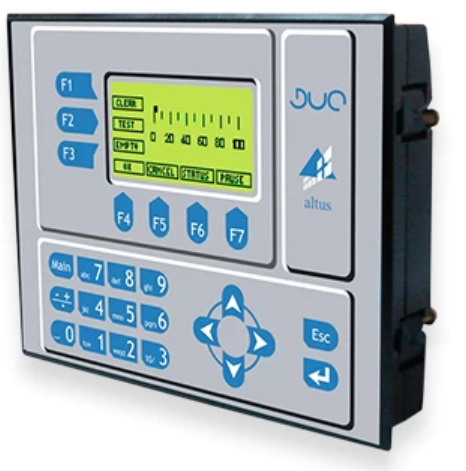
\includegraphics[scale=0.7]{figuras/altus_duo}}
	}{
		\Fonte{Altus}
	}
\end{figure}


A \textbf{série iX} é outra linha de produtos da Altus que é composta por um conjunto de \acrshort{IHM}s utilizadas como terminais de operação e visualização para aplicações industriais. É uma plataforma aberta, podendo interagir com ferramentas .NET, além da versatilidade das suas aplicações, desenvolvidas através da interface iX Developer, que podem ser executados em vários modelos de IHM dentro da mesma série.

\begin{figure}[h!]
	\centering
	\Caption{\label{fig-altus_ix_series}\acrlong{IHM} (\acrshort{IHM}) - Altus Série iX}		
	\UECEtab{}{
		\fbox{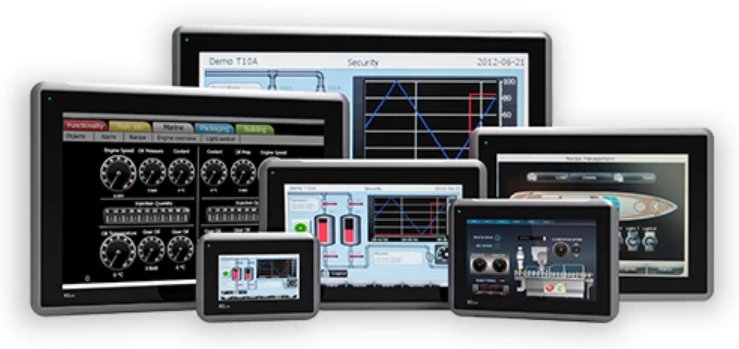
\includegraphics[scale=0.8]{figuras/altus_ix_series}}
	}{
		\Fonte{Altus}
	}
\end{figure}

A série iX bem como outras linhas de IHM, são denominadas pelo fabricante/fornecedor como Terminais Gráficos, funcionalmente menos abrangente, mas para nosso uso, equivalente. 


Os terminais que compõem a série são: iX-T4A, iX-T7A, iX-T10A, iX-T5F-2, iX-T7F-2 e iX-T10F-2, sendo eles terminais gráficos, coloridos, \textit{touchscreen} e display com tecnologia TFT \footnote{Transistor de Película Fina \cite{tecnoblog_tft}. }
De acordo com o fornecedor, este série foi descontinuada, assim, não são mais fabricados ou disponibilizados para venda ou mesmo suporte técnico. A sugestão para reposição são os teminais da linha X2-BASE, que são integralmente compatíveis com a série iX \cite{ix_t7f_2-x2_base_7}.


\section{Motivação}
\label{sec:motivacao}

A disponibilidade de equipamentos no laboratório de controle de processos, especificamente o terminal gráfico iX-T7F-2 e o CLP da Série DUO, montado em um kit didático (\acrlong{TB} - TB131), e a ausência de um procedimento de trabalho, contendo o passo-a-passo para conexão com outros equipamentos como \acrshort{CLP}s, juntamente com a necessidade da produção de um projeto de férias, motivaram a produção deste trabalho, facilitando a consolidação das competências adquiridas quanto ao uso do referido equipamento e suas utilizações nos cursos de Engenharia de Controle e Automaçãoe e Técnico em Automação Industrial.  




\section{Objetivos}
\label{sec:objetivos}


\subsection{Objetivo Geral}
\label{sec:objetivo-geral}

Proporcionar suporte básico à comunicação entre \acrshort{IHM} e \acrshort{CLP} alocados no laboratório de Controle de Processos, bem como uma atividade guiada simples para introdução à sua utilização.




\subsection{Objetivos Específicos}
\label{sec:objetivos-especificos}


	\begin{alineas}
		\item Especificar a forma de conexão entre equipamentos:
			\begin{alineas}
			\item terminal gráfico (iX-T7F-2) e \acrshort{CLP} (\acrshort{TB}131);
			\item para a transferência da aplicação(projeto) entre o computador e o terminal gráfico.
			\end{alineas}
		\item Introdução à utilização do terminal gráfico iX-T7F-2;
		\item Aplicação de comunicação entre \acrshort{CLP} (\acrshort{TB}131) e \acrshort{IHM} (ix-T7F-2).
	\end{alineas}

	\chapter{Fundamentação Teórica}
\label{cap:fundamentacao-teorica}


\section{O terminal gráfico iX-T7F-2 (\acrshort{IHM})}
\label{sec:fundamentacao-equipamentos}

O terminal gráfico ou a\acrshort{IHM} da Altus, modelo iX-T7F-2, que aqui será abordada como equipamento de estudo, é chamada pela empresa de terminal de operação, e pode-se destacar algumas de suas características gerais, conforme Tabela \ref{tab:caracteristicasgerais}. 


\begin{table}[ht!]
	\Caption{\label{tab:caracteristicasgerais}Características gerais}
	\UECEtab{}{
		\begin{tabular}{ll}
			\toprule
			Característica & iX-T7F-2 \\
			\midrule \midrule
			Tamanho da tela & 7" (154,1mm x 85,9mm) \\
			Resolução da tela & 800x480 pixels (16:9) \\
			Visor & LCD-TFT 64K cores \\
			Tipo e vida útil do \textit{Backlight} & LED 20.000h \\
			\textit{Touchscreen} & Resistivo \\
			\midrule
			Memória de aplicação & 200MB \\
			Memória RAM & 128MB \\
			Relógio de tempo-real & sim \\
			\midrule
			Tensão de alimentação & 24V (18 a 32 $V_{DC}$) \\
			Fusível interno & 2A \\
			Máxima dissipação de potência & 9,6W \\
			\midrule
			Porta USB 2.0 (400mA) & 1 \\
			Porta Ethernet 10/100 Base-T & 1 \\
			COM1 & RS-232 (RTS/CTS) \\
			COM2 & RS-422/RS-485 \\
			COM3 & RS-232 \\
			COM4 & RS-485 \\
			\midrule
			Número de Tags & 800 \\
			Número de telas & 100 \\
			Alarmes & 400 \\
			Número de controladores de comunicação & 4 \\
			\bottomrule
		\end{tabular}
	}{
		\Fonte{Terminais de operação Série iX \cite{terminais_operacao_serie_ix}}
		\Nota{As portas COM1 e COM2 são alocadas em um mesmo conector, bem como a COM3 e a COM4. Assim, ao selecionar uma das portas de comunicação, a outra é desabilitada.}
	}
\end{table}




As dimensões e os conectores podem ser vistos na representação da Figura \ref{fig:ihm_dimensions}, em que deve-se notar que as portas COM1 e COM2 compartilham o mesmo conector DB9, da mesma forma que as portas COM3 e COM4 também compartilham um único conector DB9, desta forma, ao habilitar uma delas, a outra é desabilitada. 

\begin{figure}[ht!]
	\centering
	\Caption{\label{fig:ihm_dimensions} Dimensões e conectores}
	\UECEfig{}{
		\fbox{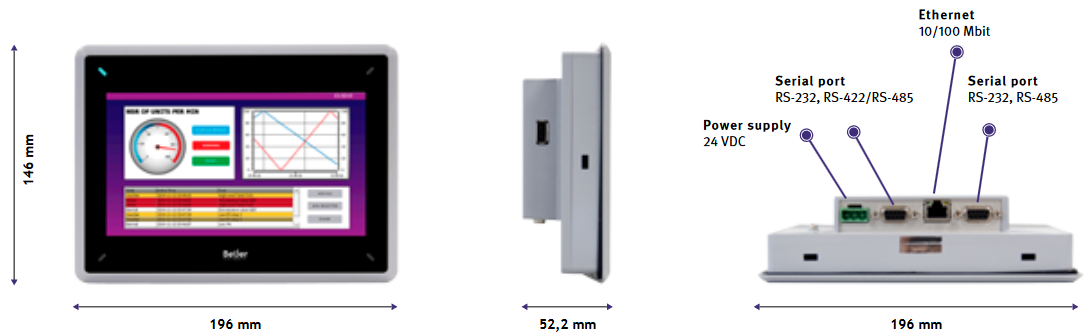
\includegraphics[width=14cm]{figuras/beijer-dimensions}}
	}{
		\Fonte{Beijer Eletronics}
	}
\end{figure}


Os terminais gráficos da Altus, são desenvolvidos e fabricados por uma empresa sueca, Beijer Electronics, Inc. que possui um foco em aplicações de comunicação, controle e interfaces homem-máquina para a industria. 
Por possuir uma abordagem transversal aos segmentos industriais, seus equipamentos destacam-se pela ampla gama de drives de comunicação disponíveis, incluindo não somente aqueles de domínio publico mas tambéms os proprietários. 
Aqui destacamos o Modbus definido pela MODICON, com os protocolos \textbf{Modbus Master RTU/ASCII} e \textbf{Modbus Slave RTU/TCP}.


A elaboração de projetos para o terminal gráfico é feita utilzando o software \textbf{iX Developer}, que pode ser obtido diretamente no site da Altus (www.altus.com.br), na aba \textbf{Suporte \& Downloads} >> \textbf{Downloads}, em \textbf{Central de Downloads} selecione somente a \textbf{Categoria: Softwares} e \textbf{Série: Série iX}. São listados os \textit{softwares}, Manuais e Apostilas disponíveis.


\subsection{Conexão para gravação de projeto no terminal gráfico/IHM}


De acordo com o documento \textbf{Terminais de Operação da Série iX} \cite{terminais_operacao_serie_ix}, o terminal gráfico pode receber um projeto para ser executado via \textit{pendrive} ou através da porta Ethernet, como ilustrado na Figura \ref{fig:pc_rot_ihm}, em que a conexão entre um computador e o terminal gráfico, possui um switch/roteador como intermediário da conexão. 
A conexão entre os dispositivos utiliza cabo de rede CAT5e e terminais seguindo o padrão EIA/TIA 568A. 


\begin{figure}[ht!]
	\centering
	\Caption{\label{fig:pc_rot_ihm}Conexão para \textit{download} da aplicação no terminal gráfico }
	\UECEfig{}{
		\fbox{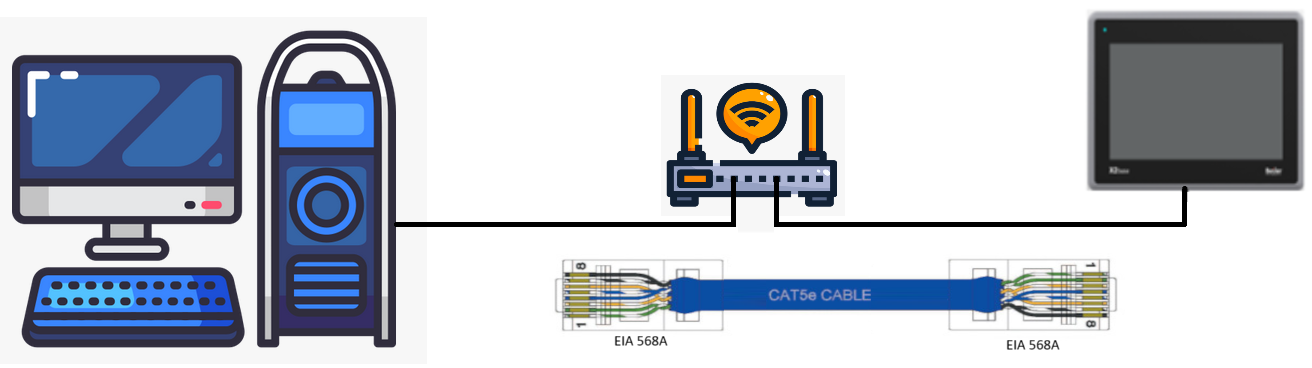
\includegraphics[width=14cm]{figuras/altus-pc_rot_ihm_cabo}}
	}{
		\Fonte{Próprio autor}
	}
\end{figure}


Da mesma forma, a Figura \ref{fig:pc_rot_ihm_wifi} ilustra a conexão feita por um notebook utilizando o \textit{Wi-Fi} como meio de comunicação. 

Note que, partindo do \textit{switch}/Roteador, cada ramo de comunicação utiliza um meio físico diferente, sendo que para o \textit{notebook} o meio é \textit{Wi-Fi} e para o terminal gráfico é cabo par-trançado direto.

O cabo par-trançado possui ambas as terminações no padrão EIA-568A, mas poderiam ser padrão EIA-568B, desde que em ambas as pontas.


\begin{figure}[ht!]
	\centering
	\Caption{\label{fig:pc_rot_ihm_wifi}Conexão via Wi-Fi para gravação de projeto no terminal gráfico}
	\UECEfig{}{
		\fbox{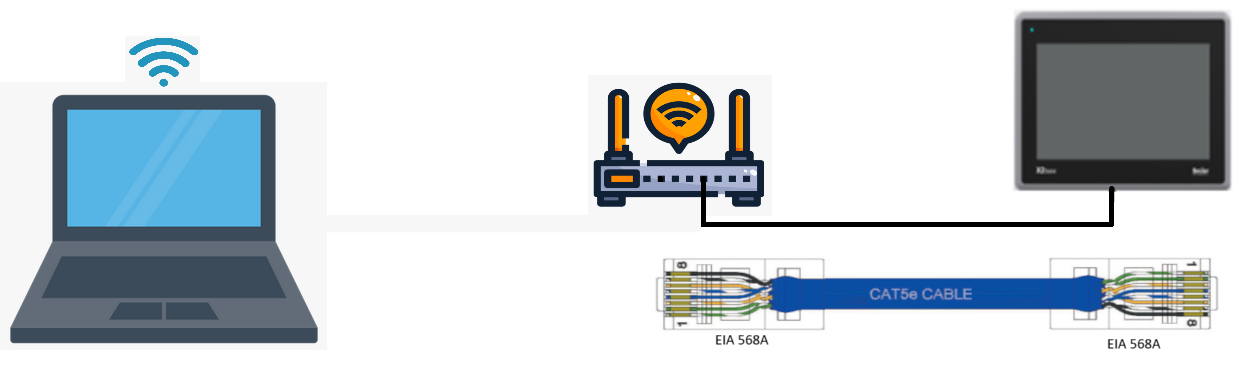
\includegraphics[width=14cm]{figuras/altus-pc_rot_ihm_wifi}}
	}{
		\Fonte{Próprio autor}
	}
\end{figure}


Pode-se ainda fazer a conexão direta entre o computador/notebook e o terminal gráfico utilizando um cabo de rede padrão crossover.

No caso do cabo de rede de par-trançado padrão crossover, uma das terminações é montada com o padrão EIA-568A enquanto a outra terminação é montada no padrão EIA-568B.



\begin{figure}[ht!]
	\centering
	\Caption{\label{fig:pc_ihm_cabocross}Conexão direta para \textit{download} de projeto no terminal gráfico}
	\UECEfig{}{
		\fbox{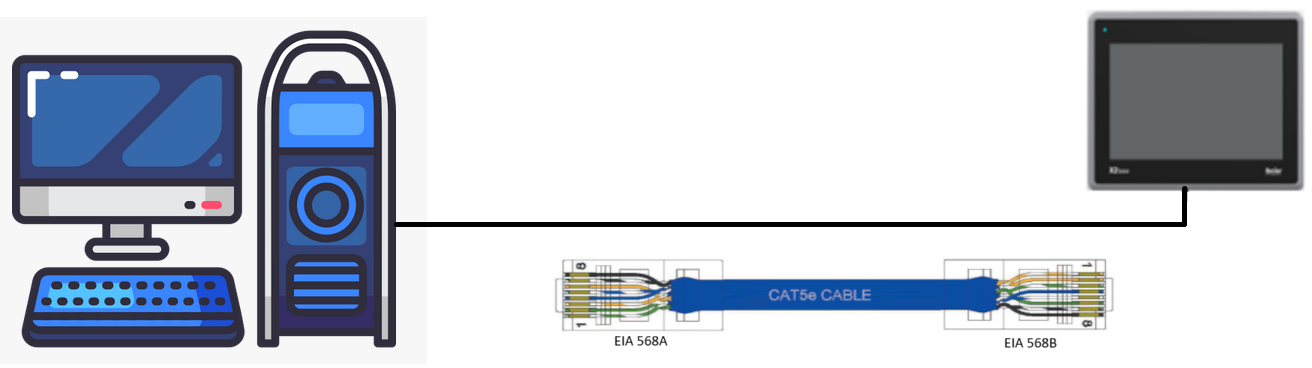
\includegraphics[width=14cm]{figuras/altus-pc_ihm_cabocross}}
	}{
		\Fonte{Base de conhecimento - Altus \cite{ixdev_download}}
	}
\end{figure}


Mais informações podem ser obtidas na Plataforma Base de conhecimento da Altus \cite{ixdev_download}, inclusive para a realização de \textit{upload} de programa contido no terminal gráfico de volta ao iX Developer.  






\section{Conexão entre o terminal Gráfico/IHM e o CLP}

A operação do terminal gráfico, execução do projeto nele gravado, ocorre mediante a sua comunicação com um controlador, normalmente um \acrshort{CLP}, mas pode ser qualquer dispositivo que implemente um dos protocolos disponíveis. 

O protocolo de comunicação que será aqui utilizado é o Modbus e o controlador é o \acrshort{CLP} da linha DUO da Altus, montado em um kit didático, o \acrshort{TB}131 (\acrlong{TB}). 

Como exemplo diferente ao \acrshort{CLP}, poderíamos utilizar uma placa de desenvolvimento contendo um microcontrolador, como um Arduino, devidamente programado e com o protocolo Modbus implementado. Esta é uma outra possibilidade com real viabilidade. 

O protocolo Modbus foi desenvolvido pela Modicom nos primórdios da automação, no final da década de 70. 
Por ser um protocolo aberto, pode ser livremente implementado pelos diversos fabricantes de equipamentos, mesmo que praticamente todos os desenvolvedores possuam o seu próprio protocolo. 
Desta forma o Modbus se tornou uma "língua franca", falada por praticamente todos os equipamentos do mercado, possibilitando assim, que em uma rede possam interagir equipamentos dos mais diversos fabricantes. 

Mais informações de forma didática sobre detalhes do protocolo Modbus podem ser encontradas no site Automação e Cartoons \cite{automacao_cartoon} ou ainda diretamente da insituição que gerencia o padrão atualmente, Modbus.org \cite{modbus_org}.




A comunicação entre a \acrshort{IHM} e o \acrshort{TB}131 pode ser realizada como ilustrado na Figura \ref{fig:connect_ihm_clp},
%
%e \ref{fig:connect_ihm_clp_cabosimples}. O meio físico aqui utilizado é RS-485, por ser de uso mais difundido em aplicações industriais.
%
conforme recomendação nos manuais da Altus \cite{connect_ihm_tb131}. 
Nela, um módulo de interface, PO8525 \cite{po8525} é utilizado entre o terminal gráfico e o controlador. 





\begin{figure}[ht!]
	\centering
	\Caption{\label{fig:connect_ihm_clp}Conexão entre IHM e CLP}
	\UECEfig{}{
		\fbox{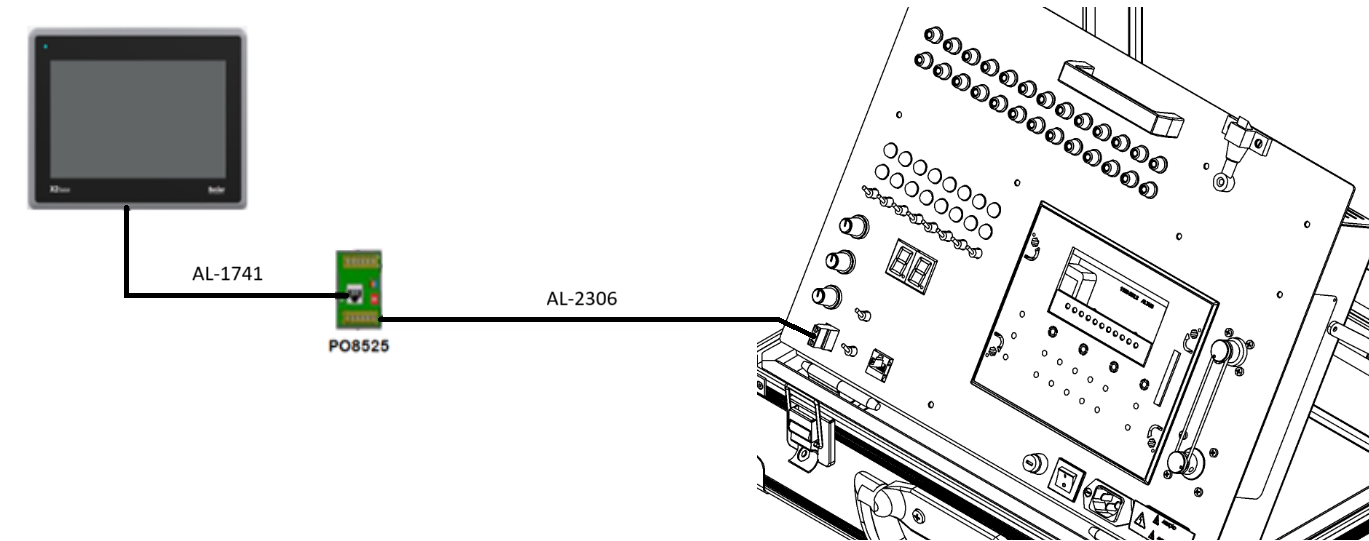
\includegraphics[width=14cm]{figuras/altus-conexao-ix_t7f_2-tb131}}
	}{
		\Fonte{Adaptado de \cite{connect_ihm_tb131}}
	}
\end{figure}


Entre o terminal gráfico e o módulo de interface, basicamente, pode-se utilizar um cabo com terminal DB9 em uma extremidade e RJ45 na outra \cite{al1741} e entre o módulo de interface e o TB131 um cabo no padrão AL-2306 \cite{al2306}.




Já entre o módulo de interface e o TB131 temos um par de cabos simples, trançado, blindado ou não, para fazer o meio físico RS-485, conforme Figura \ref{fig:connect_ihm_clp_cabosimples}. 
Desta forma, pode-se adaptar uma conexão ponto-a-ponto para estudo, utilizando um conector DB9 Macho para o terminal conectado à \acrshort{IHM} na COM2 ou COM4 (RS-485), conforme Tabela \ref{tab:caracteristicasgerais}, e para um ligação direta nos bornes do TB131, um simples decape nas pontas do fio.


\begin{figure}[ht!]
	\centering
	\Caption{\label{fig:connect_ihm_clp_cabosimples}Conexão direta entre IHM e CLP}
	\UECEfig{}{
		\fbox{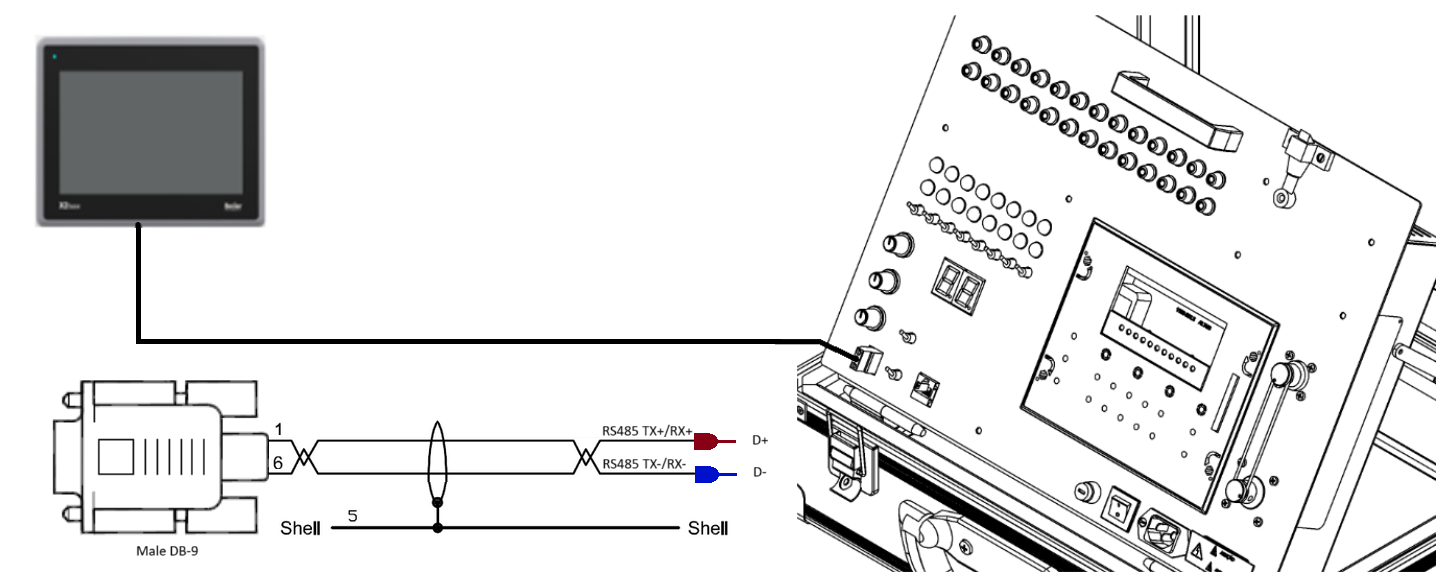
\includegraphics[width=14cm]{figuras/altus-conexao-ihm-tb131-cabosimples}}
	}{
		\Fonte{Adaptado de \cite{connect_ihm_tb131}}
	}
\end{figure}

O ponto que requer atenção é a polaridade do cabo, pois o terminal 1 do DB9 é o Sinal (+) da comuniação, enquanto o terminal 6 do DB9 é o Sinal (-), respectivamente, conectados em D+ e D- no TB131. 

Caso seja utilizado um par de cabos com malha, esta deve ser conectada ao Referencial no pino 5 do conector DB9 e no GND do conector RS-485 do TB131. 









\section{Kit didático CLP DUO - \acrlong{TB} 131 (\acrshort{TB}131)}


O kit didático possui uma interface de comunicação RS-485 que pode ser acessada habilitando a porta de comunicação serial COM2, conforme Figura \ref{fig:config_com}, através do \textit{software} de programação \textbf{Master Tool IEC}. 

A configuração da comunicação serial pode ser acessada na \textbf{Aba Recursos} >> \textbf{Configurações do CP} >> \textbf{Comunicação[FIX]} >> \textbf{COM 2[FIX]} >> Clique com o botão direito do mouse >> \textbf{Substituir elemento}.
Podem ser escolhidas as opções MODBUS Mestre, \textbf{MODBUS Escravo} ou Protocolo Genérico \cite{tb131}. 


\begin{figure}[ht!]
	\centering
	\Caption{\label{fig:config_com}Configuração de porta de comunicação Modbus}
	\UECEfig{}{
		\fbox{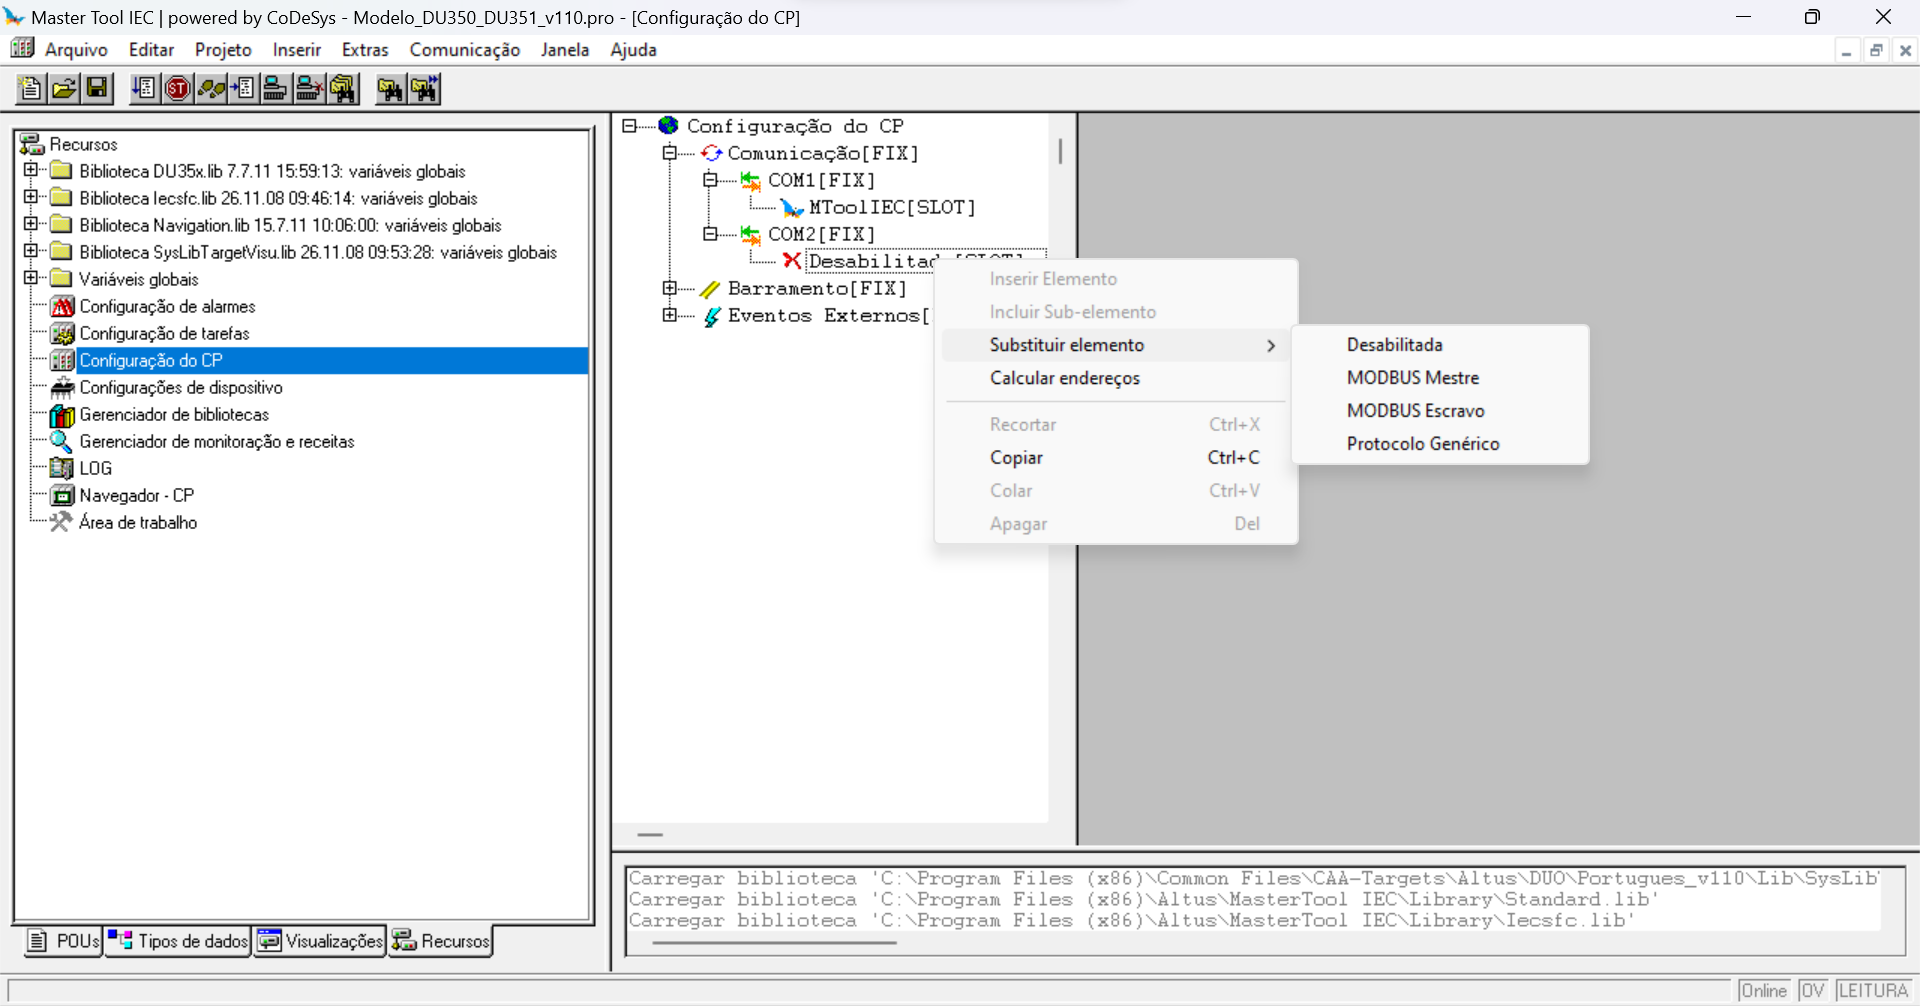
\includegraphics[width=14cm]{figuras/tb131-recursos-config-com}}
	}{
		\Fonte{Próprio autor}
	}
\end{figure}


Ao configurar a porta de comunicação como \textbf{MODBUS Escravo}, pode-se parametrizar o seu endereço como na Figura \ref{fig:com_modbus_slave_address}.

\begin{figure}[ht!]
	\centering
	\Caption{\label{fig:com_modbus_slave_address}Endereçamento de Registradores e Funções Modbus}
	\UECEfig{}{
		\fbox{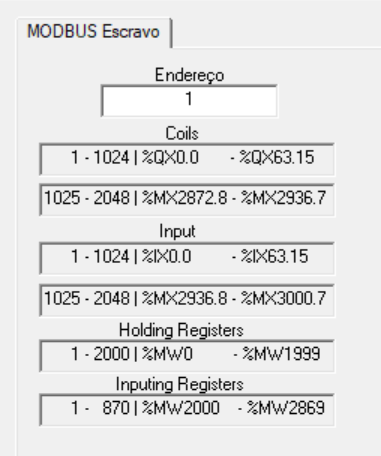
\includegraphics[width=6cm]{figuras/tb131-modbus_slave_address}}
	}{
		\Fonte{Próprio autor}
	}
\end{figure}


O endereçamento do escravo Modbus pode ser parametrizado com valor dentro do intervalo de 1 a 247, conforme o Manual de utilização da Série DUO \cite{manual_tb131}.


Para o acesso às entradas e saídas digitais endereçadas em \%IX0.0 até \%IX0.7 e \%QX1.0 até \%QX1.7, mapeadas nas chaves e LEDs no painel do TB131, não é necessária qualquer outra configuração além de habilitar a comunicação MODBUS na COM2, pois as funções Modbus acessam diretamente os endereços correspondente às entradas e saídas digitais. 

O termo Mestre-Escravo, historicamente utilizado pra denominar os elementos que se comunicam em uma rede, 
está sendo substituido pelo termo Cliente-Servidor, 
alinhando-se com as boas práticas de eliminação de linguagem inapropriada  \cite{client_server}.




%\cite{tb131}





% Manual de utilização iX-Developer \cite{ix_manual}


% \subsection{Características técnicas}

%\section{Protocolo de comunicação}
%\label{sec:fundamentacao-protocolo_comunicacao}

%\subsection{Características do sinal}

%\subsection{Configuração de comunicação Modbus}

%Os terminais de operação podem ser acessados em \cite{terminais_operacao_serie_ix}.

%Para os cabos de comunicação acesso o \cite{al1741} e \cite{al2306} bem como o derivador pode ser acessado em \cite{po8525}


% TrainingBoxDuo \cite{tb131}.

	\chapter{Fontes Principais de Informação}
\label{cap:trabalhos-relacionados}

Como fontes primárias de informações sobre o Terminal gráfico iX-T7F-2 (\acrshort{IHM}) e \acrshort{TB}131 (CLP DUO), 
recomenda-se a consulta do seu material de apoio, 
costumeiramente muito bem documentado, 
através do Site Oficial (www.altus.com.br) ou ainda das redes sociais como o Linkedin e Youtube,
em que são disponibilizados artigos relacionados aos seus equipamentos e tecnologias envolvidas. 


\begin{figure}[ht!]
	\centering
	\Caption{\label{fig:altus-linkedin} Canal da Altus S.A. no Linkedin}
	\UECEfig{}{
		\fbox{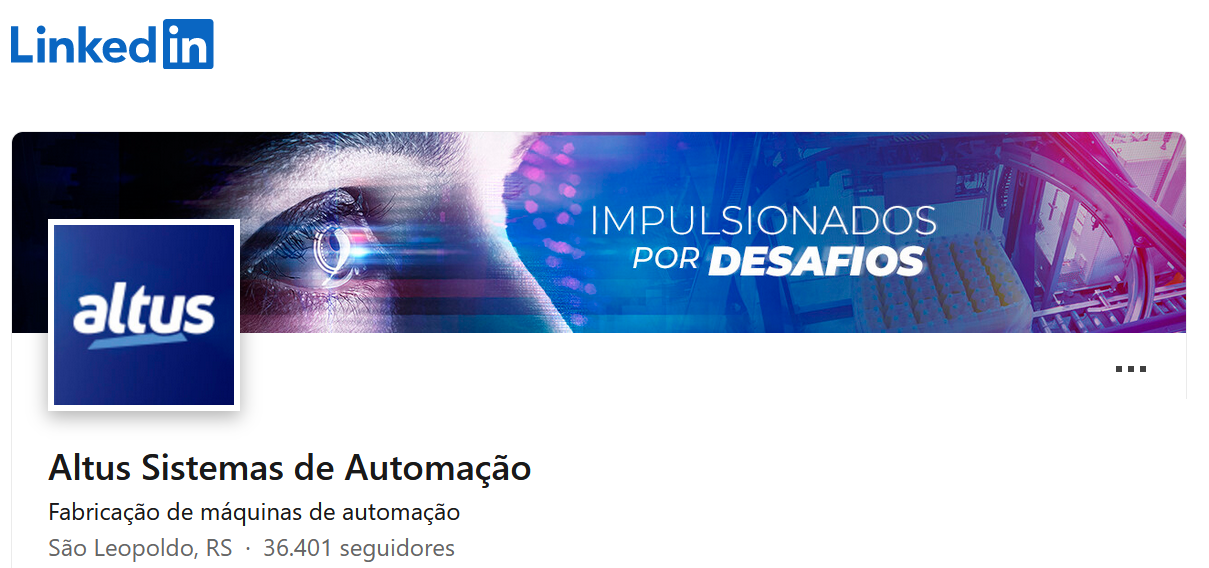
\includegraphics[width=12cm]{figuras/altus-linkedin}}
	}{
		\Fonte{Linkedin Altus \cite{altus-linkedin}}
	}
\end{figure}


No canal do Linkedin da Altus podem ser encontradas informações sobre a empresa, artigos relacionados à industria e seus ramos de atuação, assim como sobre equipamentos e suas aplicações. Ainda é possivel visualizar oportunidades de emprego oferecidas pela empresa.


\begin{figure}[ht!]
	\centering
	\Caption{\label{fig:altus-youtube}Canal da Altus S.A. no youtube}
	\UECEfig{}{
		\fbox{
\includegraphics[width=12cm]{figuras/altus-youtube}}
	}{
		\Fonte{Youtube Altus \cite{altus-youtube}}
	}
\end{figure}


No canal da Altus no Youtube estão concentrados os tutoriais para as diversas linhas de equipamentos, através de vídeos curtos e linugagem objetiva, os tutoriais oferecem uma forma prática de desenvolver o aprendizado na configuração, programação dos equipamentos da empresa. Também podem ser encontrados Webinars sobre os mais variados assuntos de tecnologia, principalmente envolvendo as técnoclogias mais atuais como Internet das Coisas - IoT (\textit{Internet of Thongs}), Segurança nas redes industriais, Sistemas de Controle e Supervisão, entro outros assuntos que fazem parte do universo Altus. 


A Beijer Electronics 
como empresa desenvolvedora de software e hardware das \acrshort{IHM}s, disponibiliza tutoriais para a sua utilização, com a vasta gama de recursos oferecidos pelo equipamento.


\begin{figure}[ht!]
	\centering
	\Caption{\label{fig:beijer-youtube}Canal da Beijer Electronics no Youtube}
	\UECEfig{}{
		\fbox{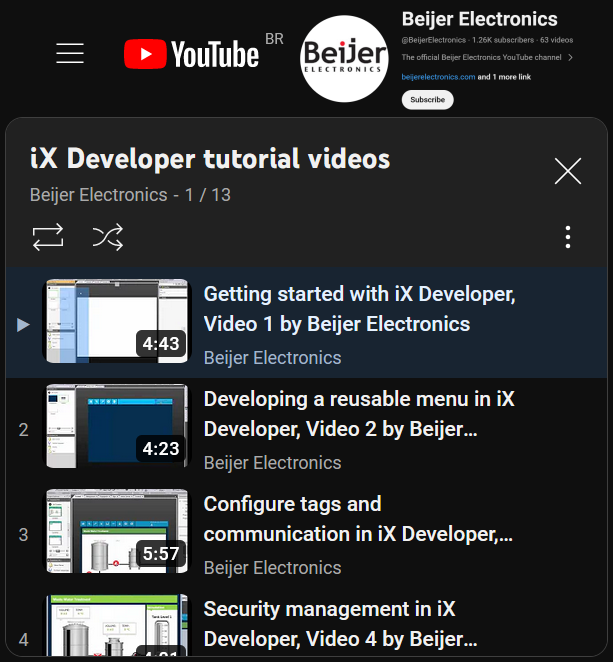
\includegraphics[width=8cm]{figuras/beijer-youtube}}
	}{
		\Fonte{Youtube Beijer Electronics \cite{beijer-youtube}}
	}
\end{figure}





Além dos canais oficiais, muitos outros podem ser acessados contendo informações, tutoriais, artigos sobre as tecnologias e sobre o uso dos equipamentos, 
com as mais variadas didáticas, que talvez te agrade mais. 
Tomando as devidas precauções quanto a legitimidade das informações e da seriedade do autor, explore as possibilidades, mas sem deixar de ter como referência as fontes originais. 





	\chapter{Especificando um projeto}
\label{chap:especificando_projeto}


Este capítulo tem como objetivo propor um projeto para o terminal gráfico iX-T7F-2, notadamente de baixa complexidade, utilizando poucos recursos, mas garantindo uma efetiva troca de informações entre o CLP e a IHM. 

É tomado como certo que os equipamentos estão conectados adequadamente, bem como o computador de desenvolvimento possui o software \textbf{iX Developer} e está em condições de efetuar o \textit{download} do projeto para a \acrshort{IHM}.

A proposta aqui presente consiste na elaboração de um painel que represente o conjunto entradas e saídas digitais e outro para as variáveis analógicas acessíveis no kit didático TB131.

A Figura \ref{fig:ativ1-telas} ilustra o conjunto de quatro telas, sendo a tela enumerada como 0, na etiqueta vermelha no canto superior esquerdo de cada tela, apenas uma tela inicial com o logo do IFSP.

\begin{figure}[ht!]
	\centering
	\Caption{\label{fig:ativ1-telas}Conjunto de telas alvo}
	\UECEfig{}{
		\fbox{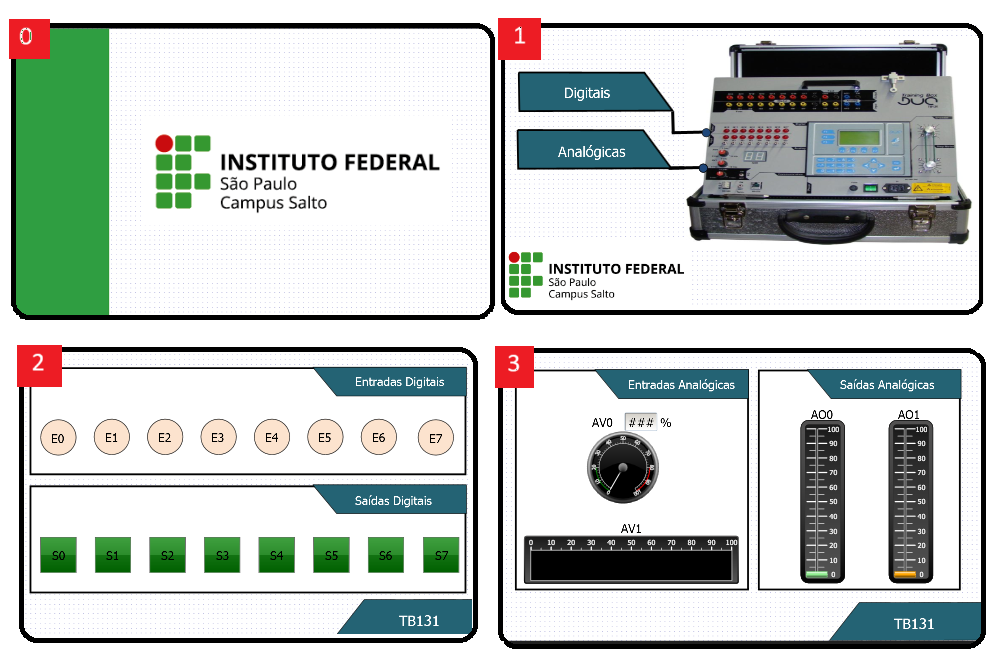
\includegraphics[width=14cm]{figuras/ativ1-telas}}
	}{
		\Fonte{Elaborado pelo autor}
	}
\end{figure}



Ao pressionar sobre o logo, ocorre a transição para a tela 1, que contem a ilustração do kit didático TB131 e as indicações dos dados analógicos e digitais. Essas indicações são botões para acesso aos dados respectivamente indicados.

Ao pressionar o botão \textbf{Digitais}, ocorre a transição para a tela 2, que contem um quadro com a indicação de \textbf{Entradas Digitais} e outro com a indicação de \textbf{Saídas Digitais}.

As entradas digitais são enumeradas de \textbf{E0} até \textbf{E7}, da mesma forma que no painal do TB131. 
Cada uma das entradas é um indicador que deve mostrar o estado lógico da respectiva entrada física do kit didático.

As saídas digitais são enumeradas de \textbf{S0} até \textbf{S7} e correspondem respectivamente às saídas \textbf{Q10} até \textbf{Q17} no painel do TB131. 
Cada uma das saídas é um botão que deve poder acionar a respectiva saída no kit didático, inclusive mudando a sua cor, indicando o estado lógico atual. 

Ao pressionar o botão no canto inferior direiro TB131, deve-se retornar à tela 1.

Ao pressionar o botão Analógicas, ocorre a transição para a tela 3, dividita também em dois quadros, um para as \textbf{Entradas Analógicas} e o outro para as \textbf{Saídas Analógicas}.

O quadro de entradas analógicas faz a leitura de duas variáveis analógicas do kit didático, associadas aos potenciômetros, AV0 e AV1. 
A variável \textbf{AV0} deve ser exibidas utilizando um \textbf{Display numérico} e um \textbf{Medidor Circular}, e a variável \textbf{AV1} deve ser exibida utilizando um \textbf{Medidor Linear} horizontal. 

Para as variáveis de saída, \textbf{AO0} e \textbf{AO1}, deve ser utilizado o componente \textbf{Slider}. 
No kit TB131, \textbf{AO0} pode ser visto através do display de 7 segmentos com dois dígitos, enquanto que o valor de \textbf{AO1} poderá ser medido com o auxílio de um multímetro entre os terminais \textbf{AO1} e \textbf{C4}. \textbf{C4} é o referencial, terra, da saída analógica \textbf{AO1}. 

Ao pressionar o botão no canto inferior direito TB131, deve-se retornar a tela 1.




	\chapter{Configuração do CLP - TB131}
\label{chap:configuracao-clp}


Esta etapa consiste em configurar o CLP, 
de modo a disponibilizar via comunicação serial, acesso aos registradores das entradas e saídas digitais e das entradas e saídas analógicas, por meio de funções do protocolo Modbus RTU. 
No caso deste CLP, 
basta apenas habilitar a porta de comunicação no modo correspondente ao Modbus Servidor RTU (Modbus Slave RTU), que as variáveis digitais já estão disponíveis, enquanto que as analógicas é necessário fazer movimentações de valores entre registradores.


\section{Configuração de comunicação Modbus}

O primeiro passo, caso não haja um projeto criado e aberto, é criar um projeto, a partir do modelo, conforme indicações da Figura \ref{fig:new_project}.

Clique em \textbf{Arquivo} >> \textbf{Novo a partir do modelo...}.

Selecione \textbf{Modelo\_DU350\_DU351\_v110} >> \textbf{Abrir}.

\begin{figure}[ht!]
	\centering
	\Caption{\label{fig:new_project}Criando um novo projeto}
	\UECEfig{}{
		\fbox{\includegraphics[width=15.6cm]{figuras/tb131-new_project }}
	}{
		\Fonte{Elaborado pelo autor}
	}
\end{figure}

Em seguida, clique com o \textbf{botão direito do mouse} em \textbf{POUs}.

Selecione \textbf{Acrescentar objeto...}. 

Selecione \textbf{Programa}, a linguagem Ladder \textbf{LD} e \textbf{OK}, 
conforme indicações da Figura \ref{fig:new_prg}.



\begin{figure}[ht!]
	\centering
	\Caption{\label{fig:new_prg}Acrescentando objeto - Programa em Ladder}
	\UECEfig{}{
		\fbox{\includegraphics[width=15cm]{figuras/tb131-new_prg}}
	}{
		\Fonte{Elaborado pelo autor}
	}
\end{figure}




Após a criação do projeto, a Figura \ref{fig:configAnalog} ilustra os passos para a configuração da comunicação com o protocolo Modbus. 


Acesse a aba \textbf{Recursos} conforme \textbf{indicador 1}.

Clique em \textbf{Configurações do CP} conforme \textbf{indicador 2}.

Na janela central aparecem opções na expansão da \textbf{Configuração do CP}: 

\textbf{Comunicação}, 
\textbf{Barramentos} e 
\textbf{Eventos externos}.

\begin{figure}[ht!]
	\centering
	\Caption{\label{fig:configAnalog}Configuração de parâmetros analógicos}
	\UECEfig{}{
		\fbox{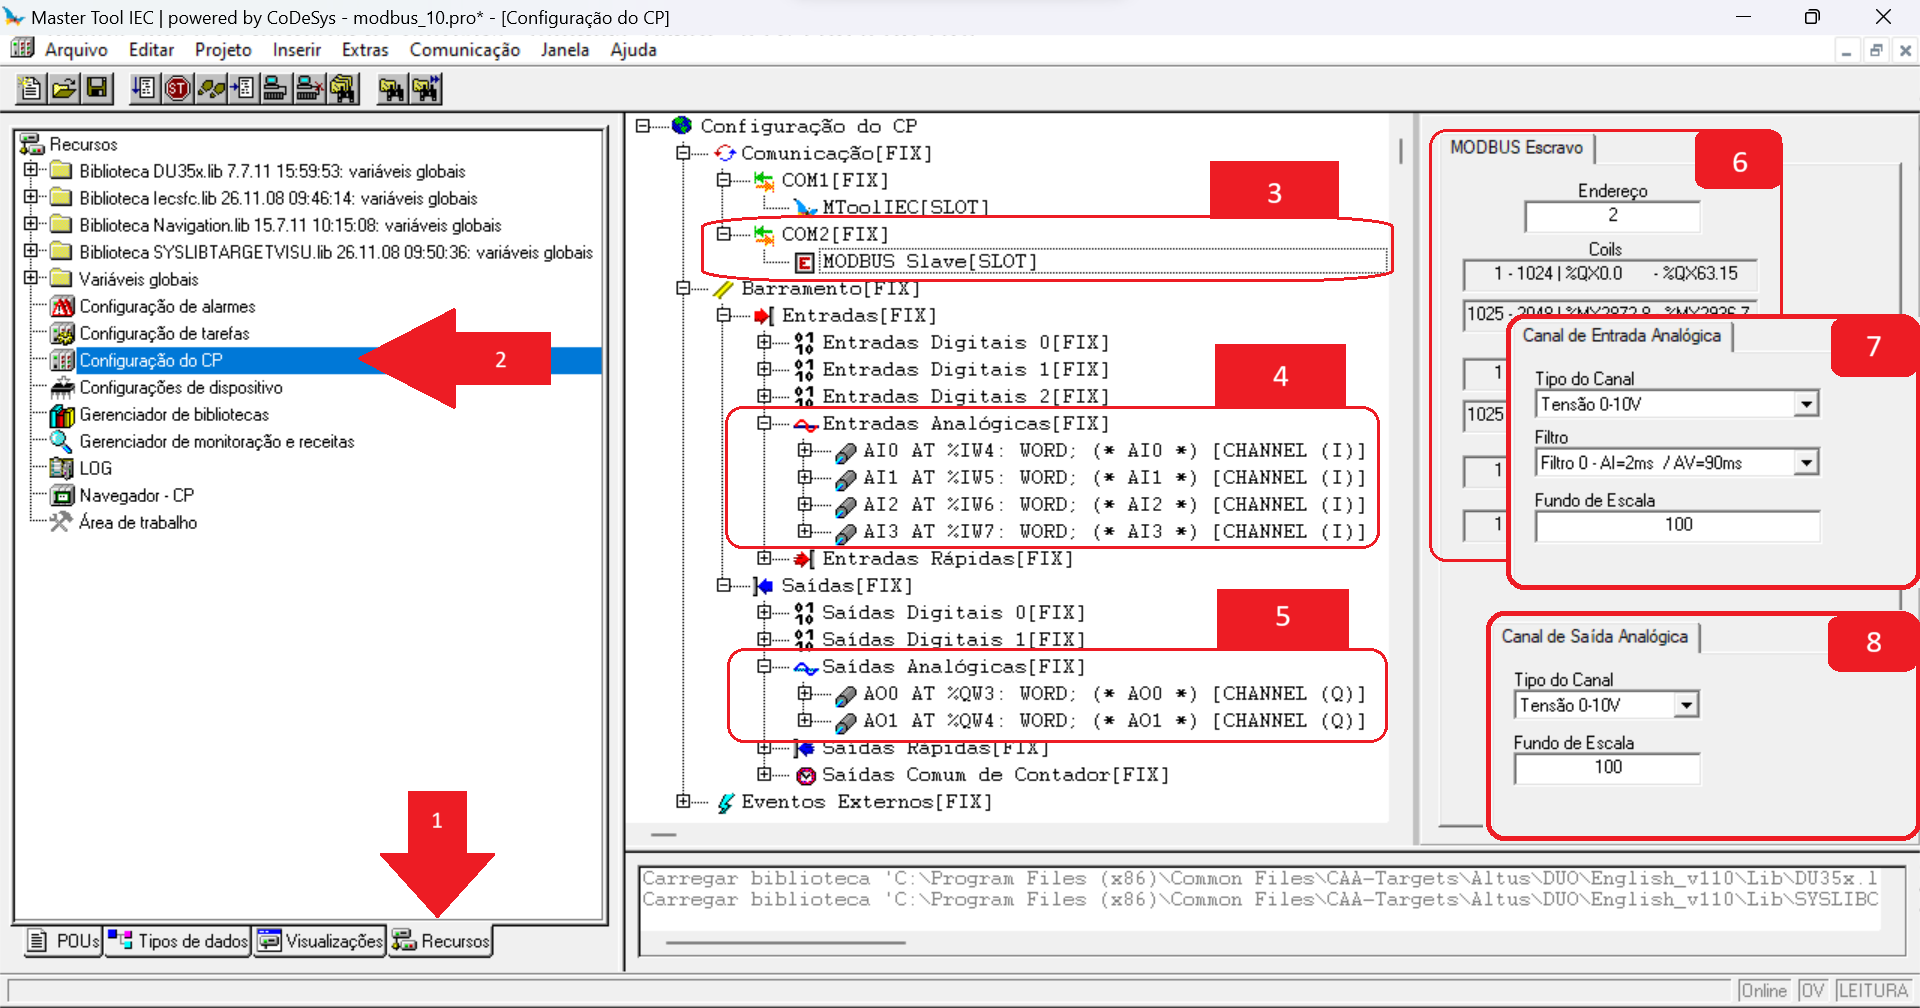
\includegraphics[width=15cm]{figuras/tb131-configAnalogModbus-n}}
	}{
		\Fonte{Elaborado pelo autor}
	}
\end{figure}


Ao expandir a opção \textbf{Comunicação}, abrem-se duas opções: \textbf{COM1} e \textbf{COM2}, sendo esta a ser configurada como \textbf{Modbus Slave}, conforme \textbf{indicador 3}. 
Como parâmetro do servidor modbus (slave), temos apenas que configurar o seu endereço, conforme \textbf{indicador 6}. 
Os demais dados são do mapeamento dos endereços das \textit{IOs} e da memória em relação às funções do protocolo utilizado.

Em \textbf{Barramento} pode-se expandir e acessar 
\textbf{Entradas} e \textbf{Entradas Analógicas}, 
conforme \textbf{indicador 4}. 
São listadas as quatro entradas analógicas (\textbf{AI0, AI1, AI2 e AI3}) e seus respectivos endereços (\textbf{\%IW4, \%IW5, \%IW6 e \%IW7}). 
Ao clicar sobre a linha de qualquer uma das entradas, é possivel configurar o canal, conforme \textbf{indicador 7}, 
para \textbf{Tensão 0-10V}, \textbf{Corrente 0-20mA}, \textbf{Corrente 4-20mA} ou ainda \textbf{Canal Desabilitado}. 
Como queremos utilizar o potenciômetro denominado \textbf{AV0}, 
que está conectado ao canal \textbf{AI0}, 
seleciona-se a opção de \textbf{Tensão 0-10V}. 
A opção de filtro é irrelevante no momento, 
bastando agora setar a opção de \textbf{Fundo de escala} para \textbf{100}. 
Este valor é arbitrário, apenas para fins didáticos, pois seu valor depende da variável do processo que está sendo monitorada.


Em \textbf{Barramento}, pode-se expandir e acessar 
\textbf{Saídas} e \textbf{Saídas Analógicas}, 
conforme \textbf{indicador 5}. 
São listadas 2 saídas analógicas, \textbf{AO0} e \textbf{AO1}, 
alocadas nos endereços \textbf{\%QW3} e \textbf{\%QW4}. 
Da mesma forma que para as entradas, 
ao clicar sobre qualquer linha de uma das saídas, 
é possível configurar o tipo de canal e o fundo de escala, conforme \textbf{indicador 8}. 

Note que todos os canais, analógicos e digitais, são independetes entre si, e possuem seus valores alocados em variáveis do tipo WORD. 





\section{ Declarando variáveis e espelhando variáveis às funções modbus}


\begin{figure}[ht!]
	\centering
	\Caption{\label{fig:insert_function_en}Inserção de funções para manipulação de dados}
	\UECEfig{}{
		\fbox{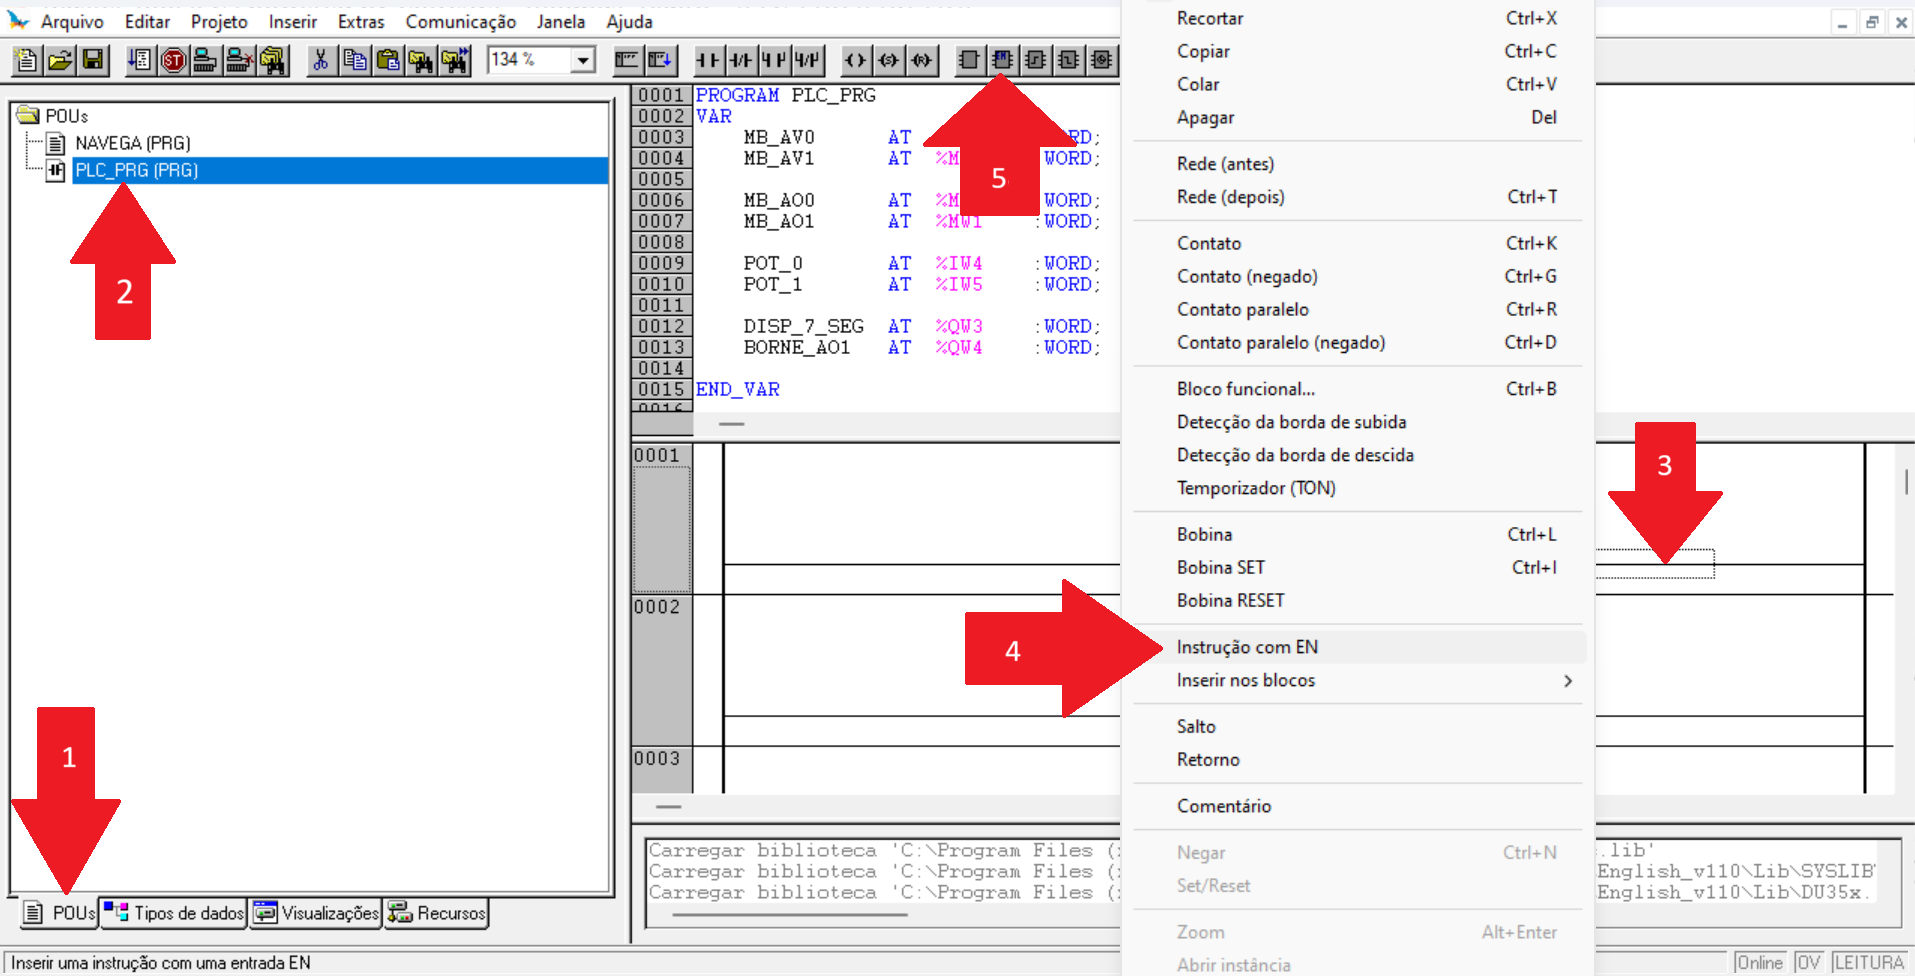
\includegraphics[width=14cm]{figuras/tb131-insert_function_en-n}}
	}{
		\Fonte{Elaborado pelo autor}
	}
\end{figure}


Após a definição da porta e do protocolo de comunicação, 
e da identificação dos canais de entrada e saída analógicos, 
retorna-se à aba do programa, 
conforme \textbf{indicação 1} da Figura \ref{fig:insert_function_en}, 
clicando na \textbf{indicação 2}.


As variáveis utilizadas podem ser definidas conforme forem sendo inseridas e utilizadas no código, ou ainda pode-se declarar todas as variáveis antes de iniciar a inserção dos blocos do programa. 


A Figura \ref{fig:declaracao_vars} ilustra a declaração de variáveis conforme serão utilizadas. 
Note que as variáveis, cujos nomes começam com 'MB\_', 
correspondem ao endereços do protocolo modbus. 
As demais variáves correspondem aos periféricos do TB131, 
POT para os potenciômetros e as saídas com os nomes explícitos: 
DISP\_7SEG e BORNE\_AO1.


\begin{figure}[ht!]
	\centering
	\Caption{\label{fig:declaracao_vars}Declaração de variáveis}
	\UECEfig{}{
		\fbox{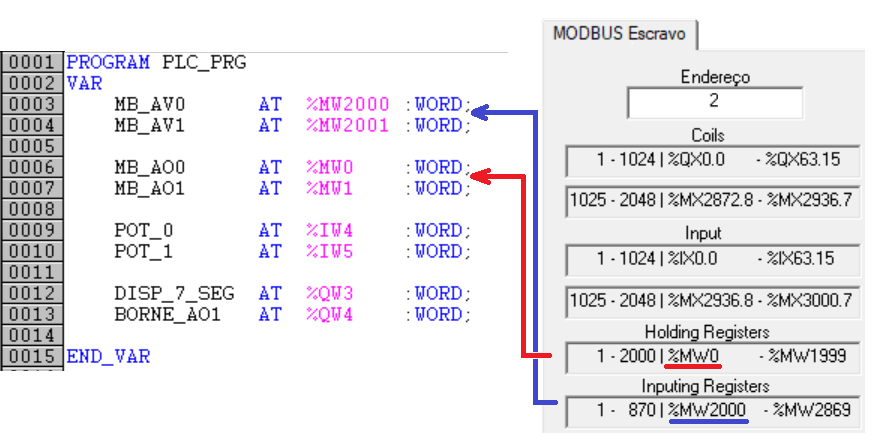
\includegraphics[width=14cm]{figuras/tb131-progCLP_vars-n-m}}
	}{
		\Fonte{Elaborado pelo autor}
	}
\end{figure}


Após a declaração das variáveis, 
é o momento de inserir no programa, 
os elementos que farão a movimentação dos dados 
dos endereços de hardware para 
os endereços das funções da comunicação modbus. 

O \textbf{indicador 3} da Figura \ref{fig:insert_function_en}, 
ilustra o local a ser inserida uma instrução com habilitação, 
ao clicar com o botão direito do mouse, conforme \textbf{indicador 4}. 
Ou ainda, ao clicar no ícone do \textbf{indicador 5}.


A Figura \ref{fig:funcoes_analog} ilustra o uso da função 
\textbf{MOVE} para transferir informação das entradas analógicas 
para os endereços correspondetes às funções de leitura no 
protocolo Modbus, bem como, 
dos endereços de escrita das funções Modbus para as saídas analógicas. 

\begin{figure}[ht!]
	\centering
	\Caption{\label{fig:funcoes_analog}Espelhamento de parâmetros analógicos para comunicação Modbus}
	\UECEfig{}{
		\fbox{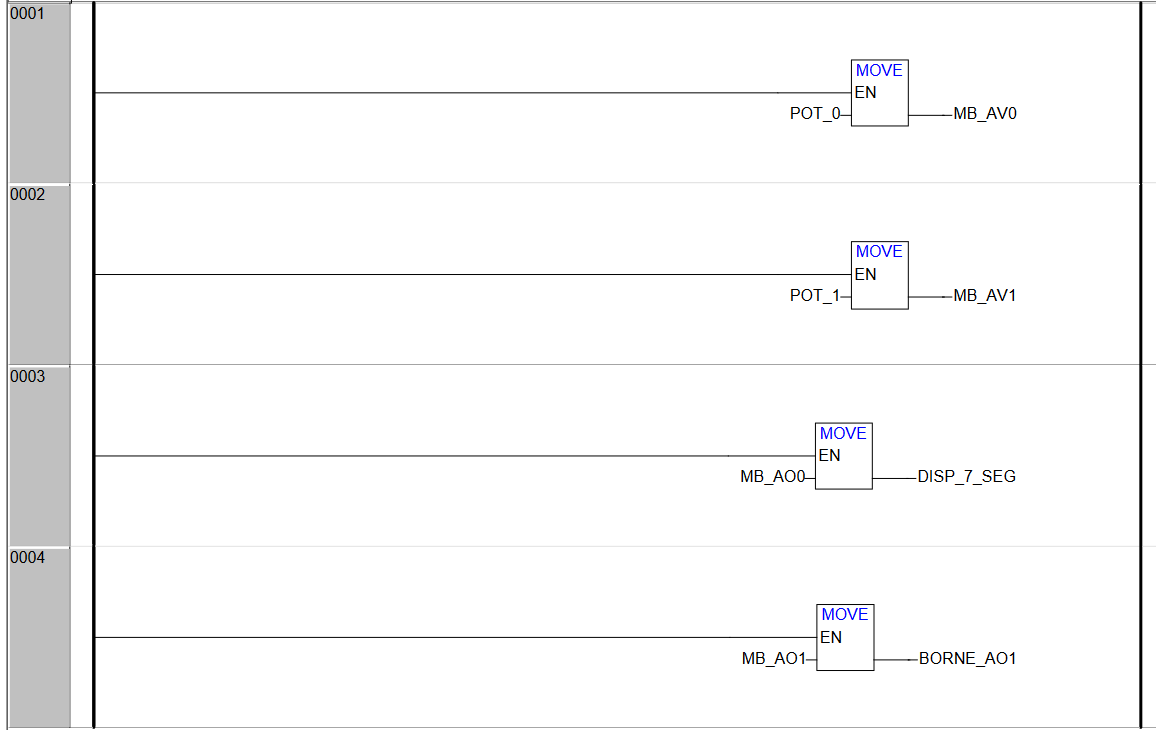
\includegraphics[width=14cm]{figuras/tb131-progCLP_analogReg}}
	}{
		\Fonte{Elaborado pelo autor}
	}
\end{figure}


Note que em todos os casos, 
a entrada \textbf{EN}, habilitação, 
está conectada e ligada direto à fonte de sinal, 
tornando todos os blocos habilitados de forma ininterrupta. 


Na primeira rede do programa, 
acontece a transferência do \textbf{POT\_0}, 
que corresponde ao endereço \textbf{\%IW4}, 
ou seja, a entrada analógica \textbf{AI0} para o \textbf{MB\_AV0},
declarada no endereço \textbf{\%MW2000}, 
que de acordo com a Figura \ref{fig:com_modbus_slave_address}, 
é o primeiro endereço da função \textbf{\textit{Inputing Register}}.

Na segunda rede do programa, 
de forma anaáloga à primeira rede, 
transfere-se o valor da segunda entrada analógica para o endereço correspondente Modbus.

Na terceira rede do programa, 
ocorre a transferência de \textbf{MB\_AO0}, 
que corresponde ao endereço \textbf{\%MW0}, 
primeiro endereço da função Modbus 
\textbf{\textit{Holding Register}}. 
Como recebedor deste valor via comunicação Modbus temos o 
\textbf{DISP\_7\_SEG}, alocado no endereço \textbf{\%QW3}, 
vinculado ao par de displays de sete segmentos no TB131. 

Na quarta rede do programa, 
de forma análoca à terceira rede, 
a trasferência do segundo endereço da função modbus para a segunda saída analógica do CLP, 
conectada no borne \textbf{AO1}, que pode ser verificada com o auxílio da utilização de um votímetro. 




\section{Compilação do programa}

Após todas as variáveis estarem declaradas e devidamente carregadas, 
recomenda-se realizar a compilação do programa. 
A compilação consiste no processamento do que foi realizado até o momento, 
de forma a garantir a consistência da sintaxe do projeto. 

Para realizar a compilação do projeto, 
acesse a aba \textbf{Projeto}, 
conforme \textbf{indicador 1} na Figura \ref{fig:compilacao} 
e clique em \textbf{Compilar tudo}, conforme \textbf{indicador 2}. 
Ao final da compilação, deve aparecer a resposta conforme o \textbf{indicador 3}, apresentando \textbf{0 erro(s) e 0 aviso(s)}. 
Caso algum erro seja exibido, verifique o comentário para ter um indicativo do que não está de acordo. 
Corrija e compile tudo novamente. 


\begin{figure}[ht!]
	\centering
	\Caption{\label{fig:compilacao}Compilação do programa}
	\UECEfig{}{
		\fbox{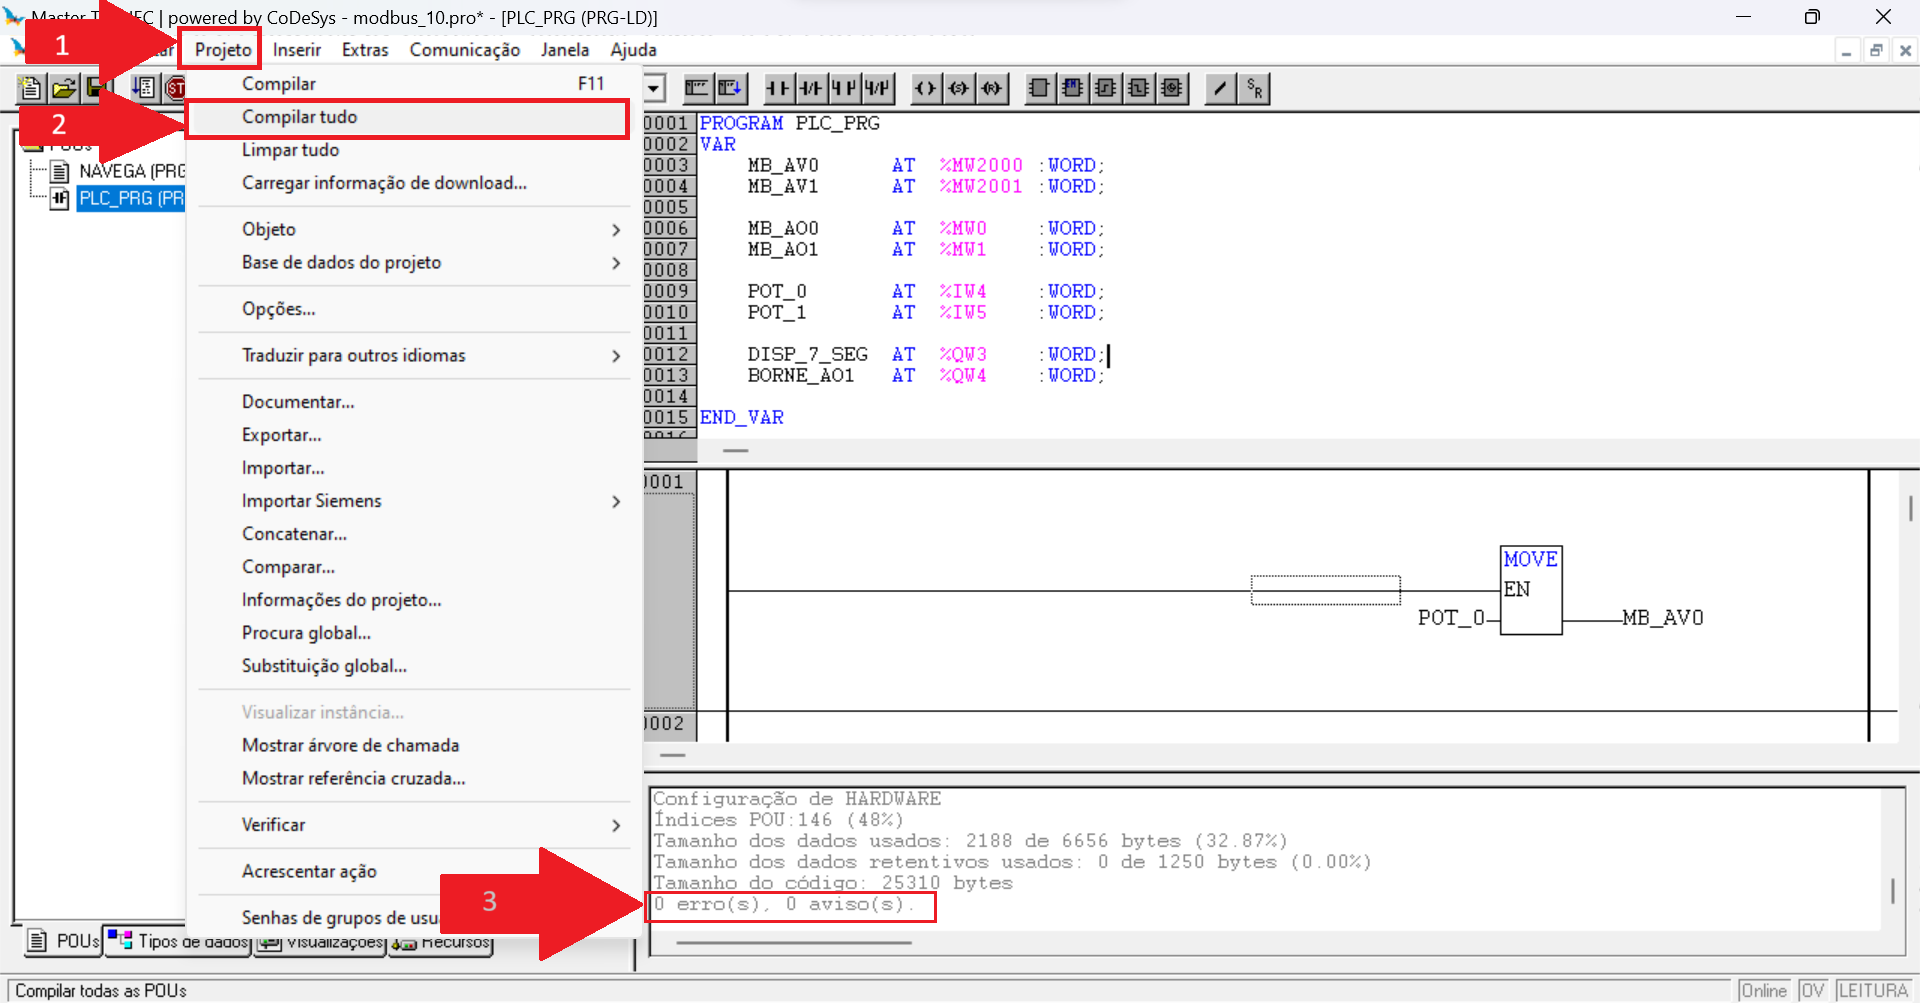
\includegraphics[width=14cm]{figuras/tb131-compile-n}}
	}{
		\Fonte{Elaborado pelo autor}
	}
\end{figure}


Ao clicar na opção \textbf{Compilar}, 
apenas aquilo que foi alterado é compilado, 
o restante do código se mantém. 
Ao clicar em \textbf{Compilar tudo}, 
todos os arquivos auxiliares são reconstruídos, 
e o projeto é processado por inteiro, 
como se não tivesse sido compilado anteriormente. 


\section{Transferência do projeto compilado}

Com o projeto compilado por completo e sem erros, 
é hora de verificar a comunicação entre o computador e o CLP. 

Clique na aba \textbf{Comunicação}, conforme o \textbf{indicador 1} da Figura \ref{fig:parametro_comunicacao}. 

Em seguida verifique se o \textbf{Modo Simulação} está desabilitado, conforme \textbf{indicador 2}. 



\begin{figure}[ht!]
	\centering
	\Caption{\label{fig:parametro_comunicacao}Configuração de parâmetros de comunicação }
	\UECEfig{}{
		\fbox{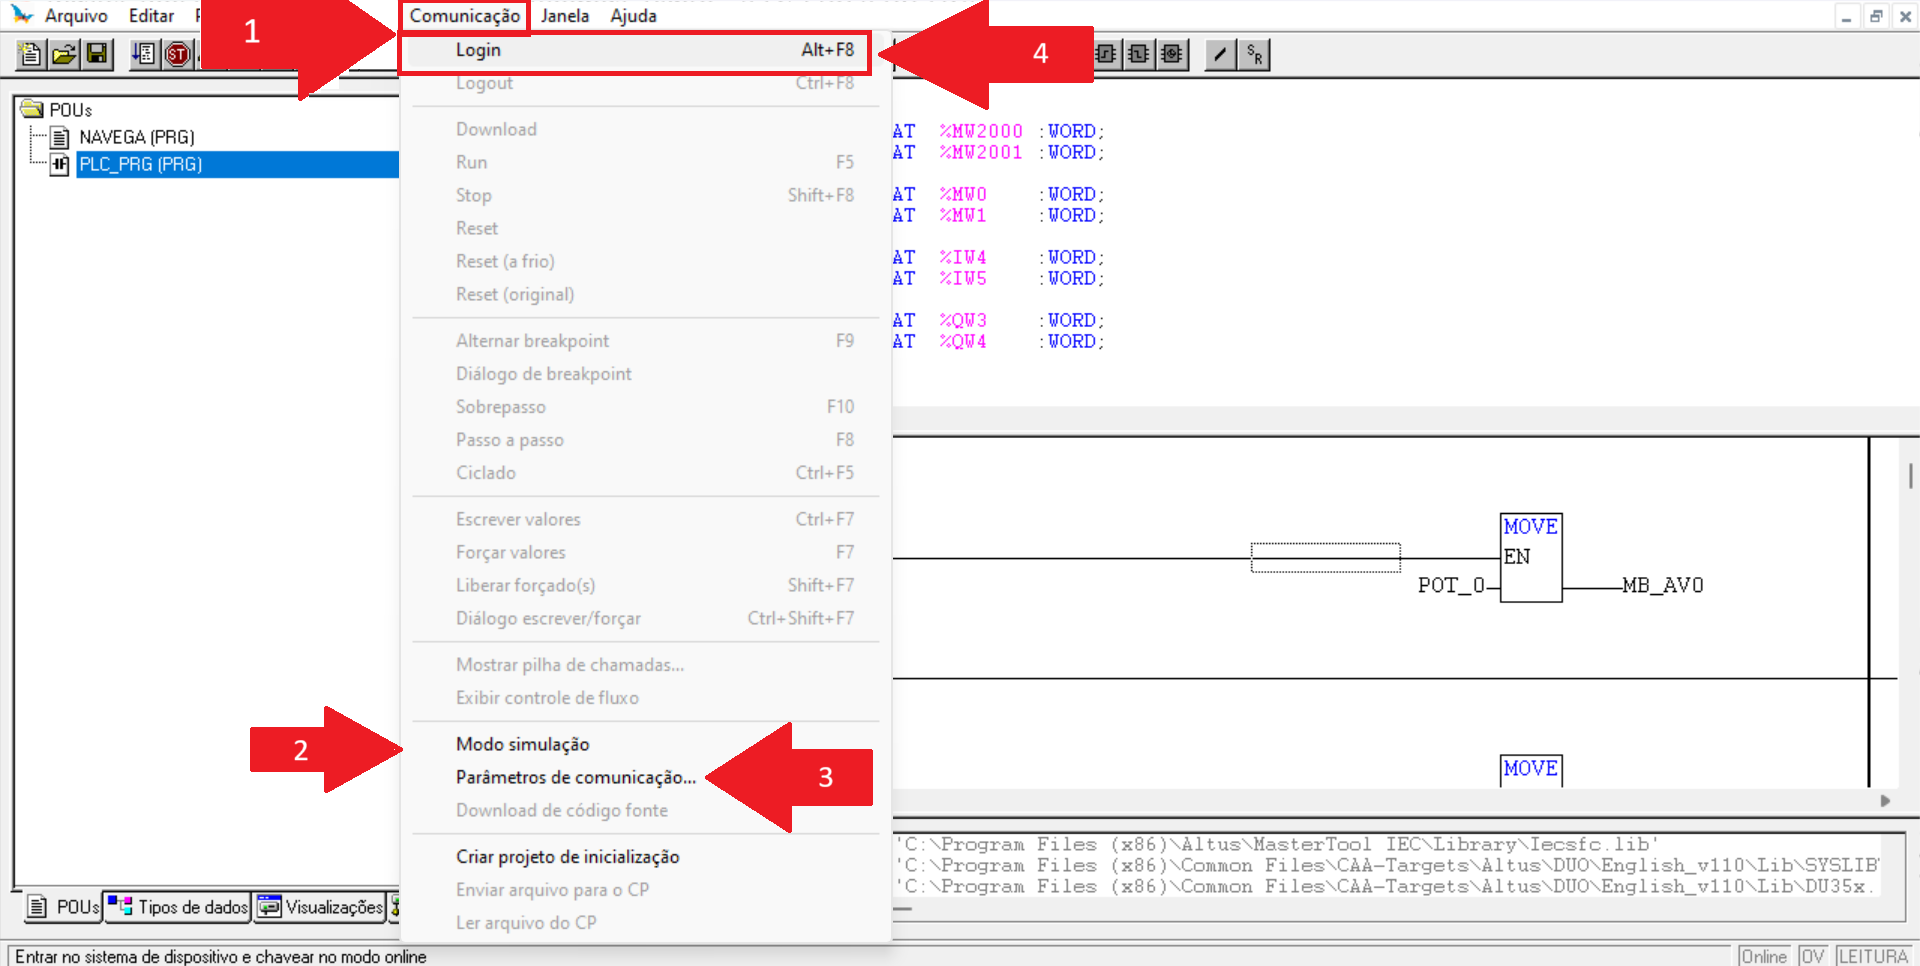
\includegraphics[width=14cm]{figuras/tb131-parametro_comunicacao-n}}
	}{
		\Fonte{Elaborado pelo autor}
	}
\end{figure}


Verifique os parâmetros de comunicação, 
conforme \textbf{indicador 3}.
Estando tudo correto, clique em \textbf{login}, conforme \textbf{indicador 4}. 


\begin{figure}[ht!]
	\centering
	\Caption{\label{fig:param_com_serial}Parâmetros de comunicação da porta Serial}
	\UECEfig{}{
		\fbox{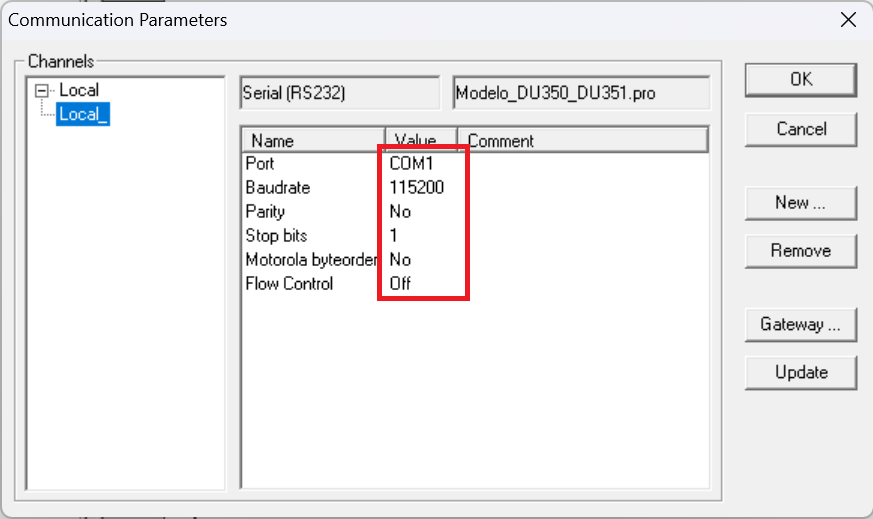
\includegraphics[width=14cm]{figuras/tb131-parametro_comunicacao_set-n}}
	}{
		\Fonte{Elaborado pelo autor}
	}
\end{figure}


Ao realizar o login de um projeto com a compilação diferente do que está gravado no CLP, 
aparece a mensagem para a retransmissão do programa executável, 
de modo a que possa ser realizado o monitoramento em tempo real das variáveis do CLP.


Ao acessar os \textbf{parâmetros de comunicação}, 
deve-se atentar principalmente para a \textbf{porta} e a \textbf{taxa de transmissão (\textit{baud rate})}. 
Para o ajuste desses valores, selecione a variável que se quer alterar com um \textbf{clique duplo} e o ajuste é realizado com as \textbf{setas do teclado}, para cima e para baixo.



\section{Exibir variáveis na IHM integrada - TB131}


Como uma forma redundante, 
as variáveis analógicas são exibidas no display gráfico do CLP. 
A Figura \ref{fig:display_design} ilustra no \textbf{indicador 1} a aba para a composição gráfica da tela. 
O \textbf{indicador 2} aponta para a tela principal, 
que é criada por padrão em todos os projetos. 
Como a exploração deste display está fora do escopo deste trabalho, 
aqui é abordada apenas a inserção de visualização de variáveis. 


\begin{figure}[ht!]
	\centering
	\Caption{\label{fig:display_design}Inserindo tela gráfica no TB131}
	\UECEfig{}{
		\fbox{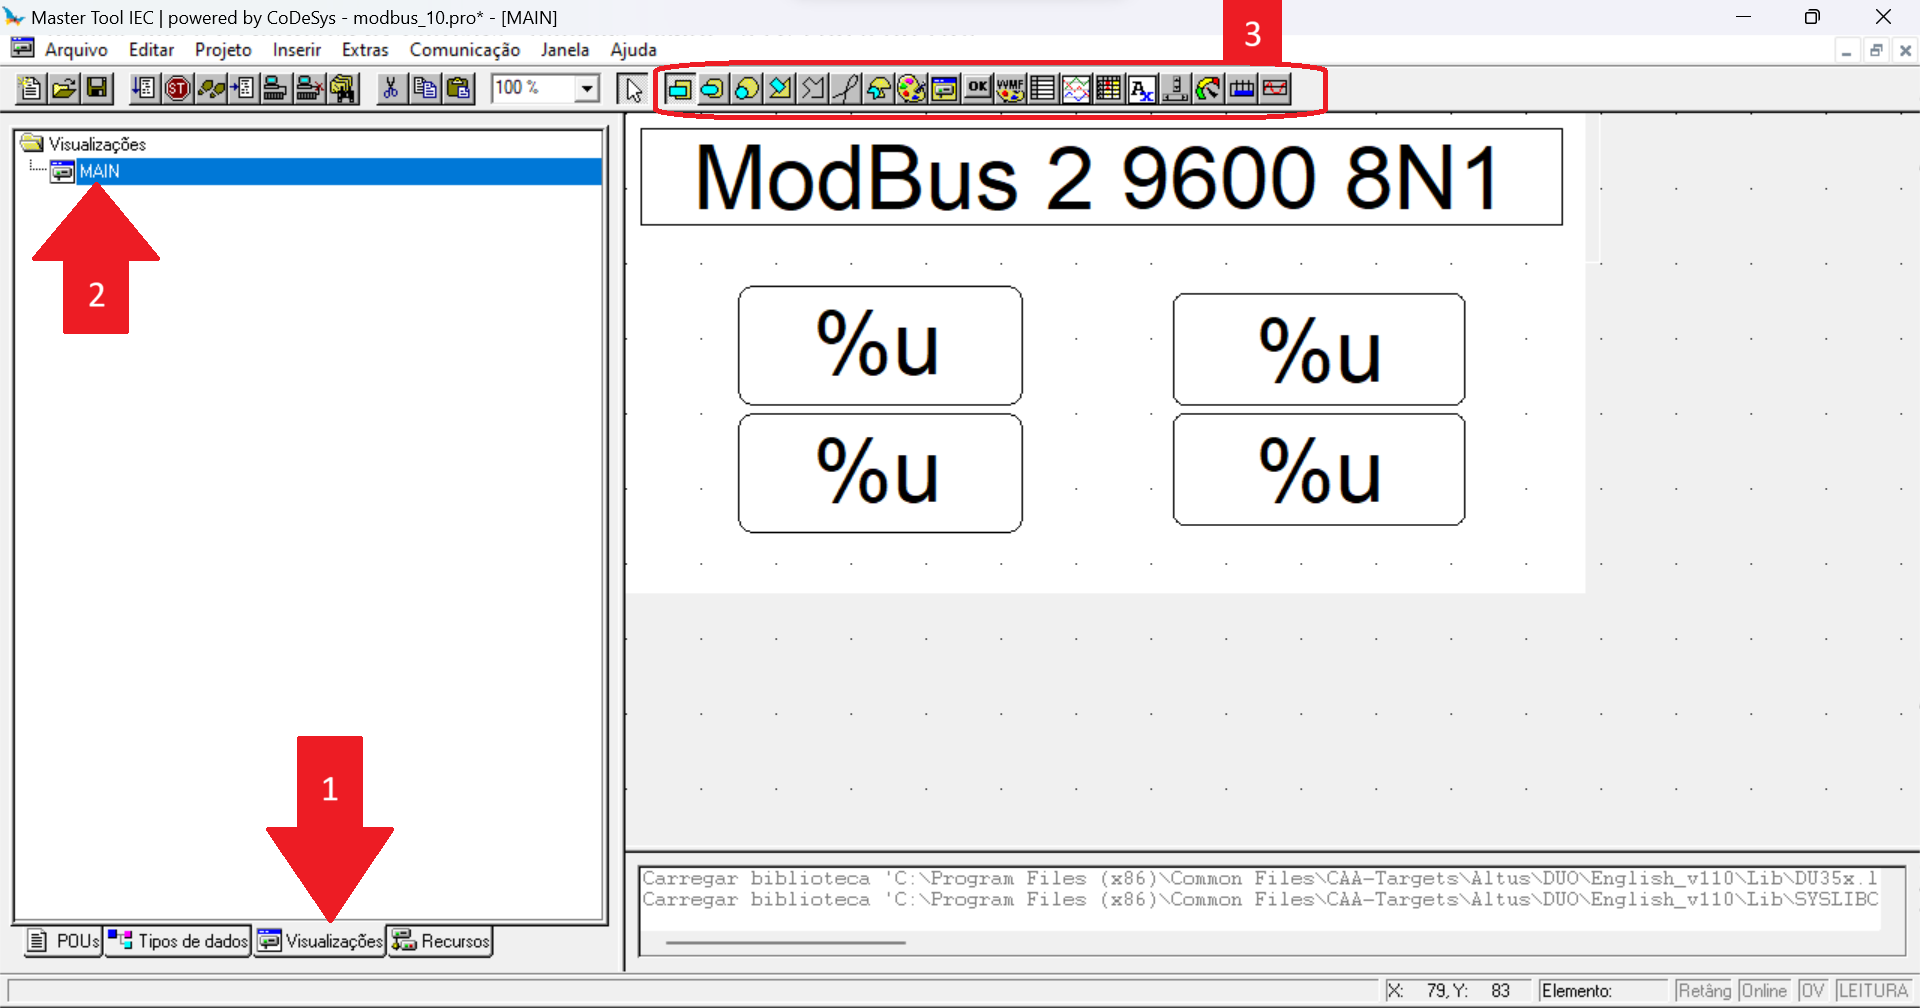
\includegraphics[width=14cm]{figuras/tb131-display_design-n}}
	}{
		\Fonte{Elaborado pelo autor}
	}
\end{figure}


Utilizando basicamente a ferramenta \textbf{Retângulo}, 
que é a primeira ferramenta à esquerda, mostrada pelo \textbf{indicador 3}, são inseridos elementos para o cabeçalho e a exibição das quatro variáveis analógicas utilizadas. 
 
Para o cabeçalho, 
ocorre apenas uma edição com a inserção do texto simples, 
ao clicar sobre o elemento, 
selecionar a opção \textbf{Texto} e na caixa de conteúdo inserir o texto do cabeçalho.
Neste caso foram inseridos os dados básicos da comunicação modbus, 
o número do servidor, \textbf{Slave=2}, 
a taxa de comunicação, \textbf{baud rate = 9600} e o complemento de \textbf{8 bits, sem paridade e um stop bit}, 
representado por \textbf{8N1}.

Para a inserção de variáveis, 
é necessário indicar na caixa de \textbf{Conteúdo} da categoria \textbf{Texto} o formato do dado a ser exibido, 
conforme indicação na Figura \ref{fig:display_var_type}.


\begin{figure}[ht!]
	\centering
	\Caption{\label{fig:display_var_type}Configurando a exibição de um dado numérico}
	\UECEfig{}{
		\fbox{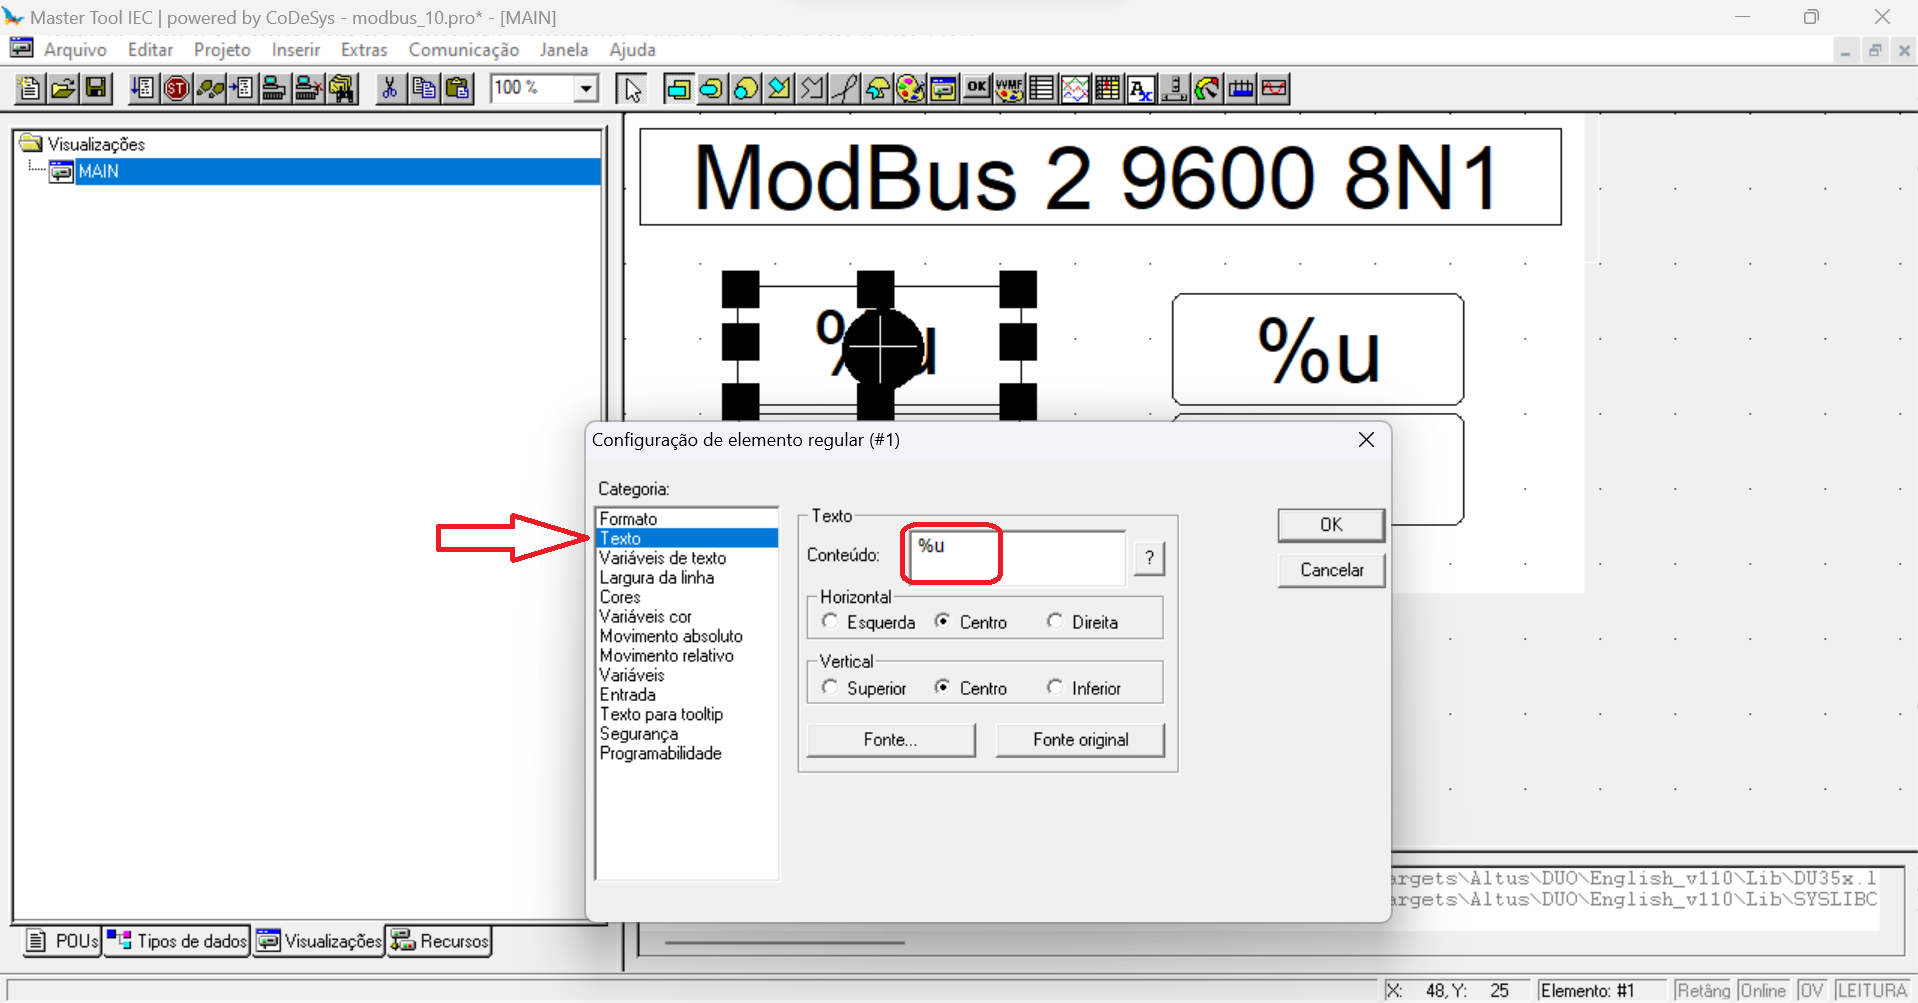
\includegraphics[width=13cm]{figuras/tb131-display_var_type-n}}
	}{
		\Fonte{Elaborado pelo autor}
	}
\end{figure}

Em seguida é necessário indicar a fonte do dado, 
como mostra a Figura \ref{fig:display_var}. 
Em \textbf{Categoria} selecione \textbf{Variáveis} e 
posicione o cursor no campo de edição de \textbf{Texto} 
pressionando em seguida a tecla \textbf{F2}. 
O assistente de entrada é aberto com as \textbf{Expressões de monitoração}. 
Expandindo a opção do programa, como \textbf{indicador 3}, 
são exibidas as variáveis já declaradas no programa, 
conforme destacado pelo \textbf{indicador 4}. 



\begin{figure}[ht!]
	\centering
	\Caption{\label{fig:display_var}Definindo a variável a ser exibida}
	\UECEfig{}{
		\fbox{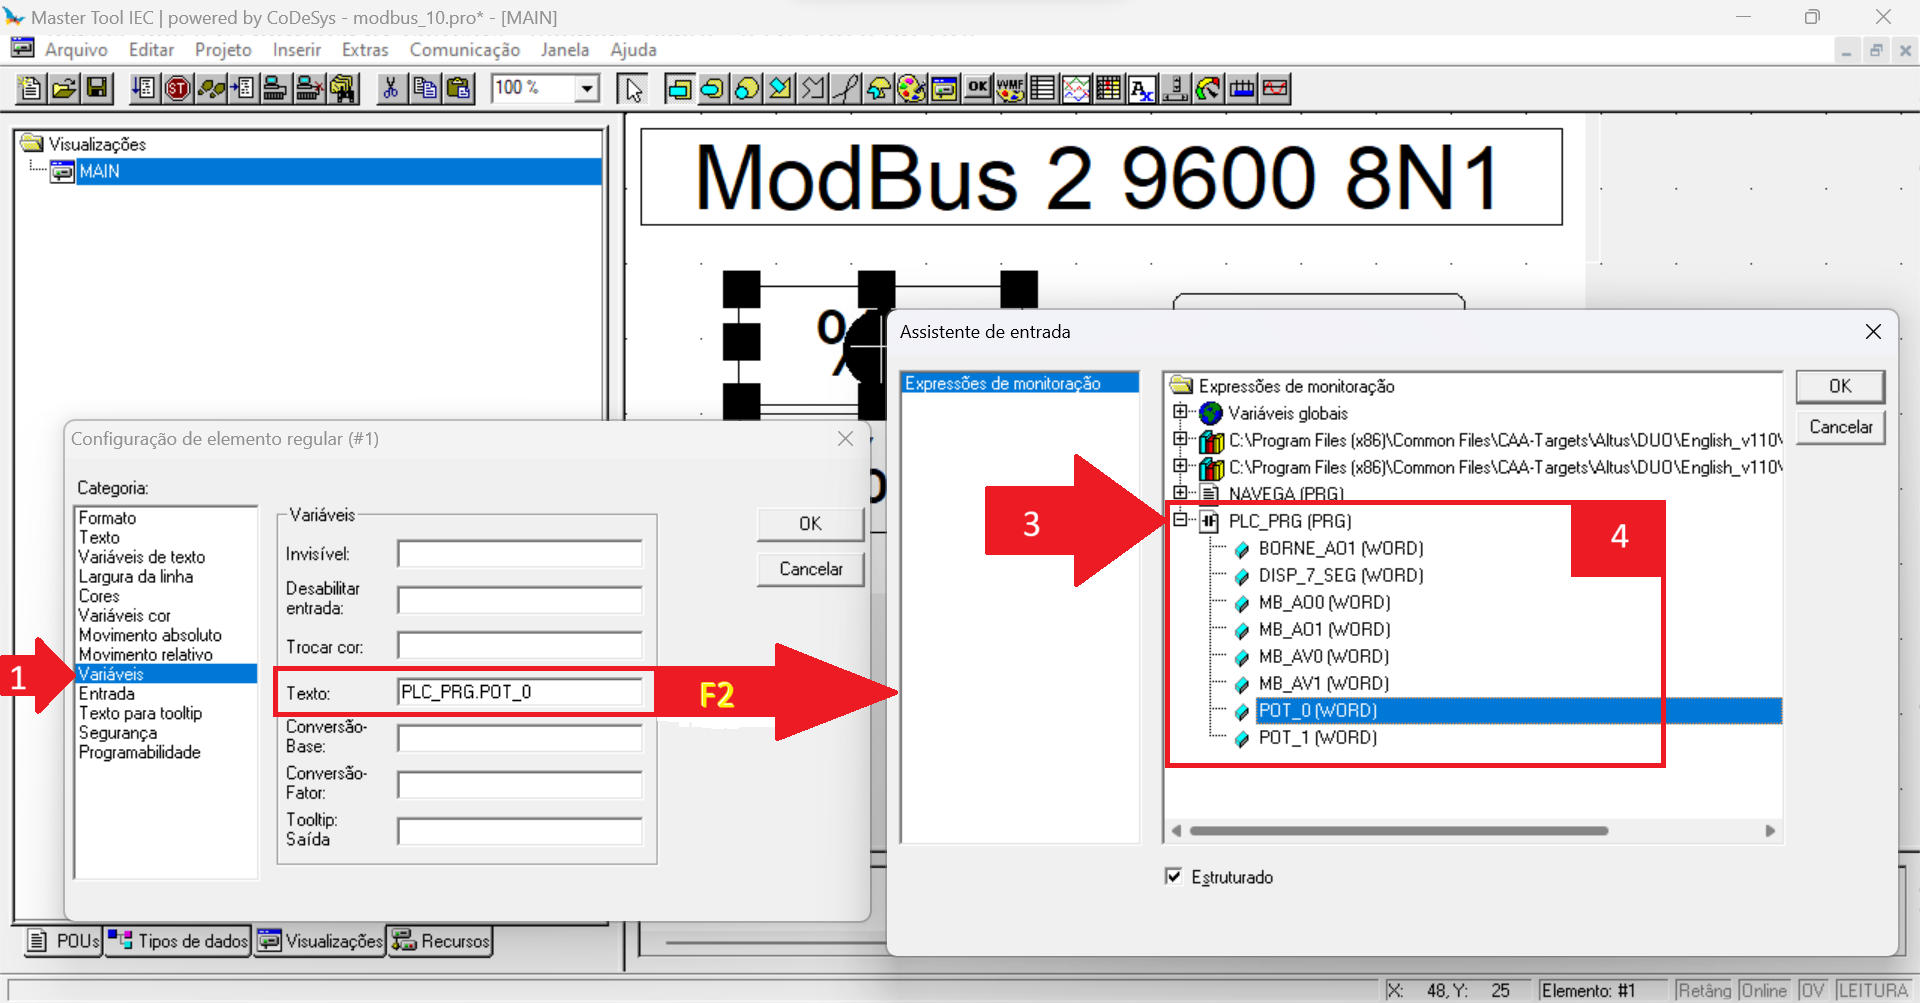
\includegraphics[width=13cm]{figuras/tb131-display_var-n}}
	}{
		\Fonte{Elaborado pelo autor}
	}
\end{figure}

Após variável selecionada é só clicar em 'OK' nas telas em aberto e repita o processo para as demais variáveis que serão exibidas na tela. 
Em seguida, faça a compilação do projeto e o download para carregar o projeto completo no CLP. 



	\chapter{Programando o Terminal Gráfico/IHM}
\label{chap:resultados}


A programação do terminal gráfico pode ser tão comlexa quanto mais recursos forem utilizados, 
passando por sistemas de identificação de usuários, 
conexão com banco de dados, 
validação de informações, 
multiplas conexões, 
segurança, 
entre outras possibilidades que o software de programação permite. 
A abordagem aqui tem o intuito de promover os primeiro passos com o uso da ferramenta, 
a criação das primeiras telas, 
a navegação e a acomunicação com um controlador. 
Sendo assim, são abordadas apenas as etapas de criação do projeto,
configuração do controlador através das TAGs e 
do protocolo de comunicação, 
a elaboração de telas de navegação e visualização de informações e
o envio do projeto para o terminal gráfico que estamos trabalhando.


\section{Criando um projeto}

A criação de um projeto para o terminal gráfico da série iX, 
entre outras, 
é o iX Developer que pode ser baixado gratuitamente em 
\cite{terminais_operacao_serie_ix}, 
com a possibilidade de uso completo pelo período de teste de 30 dias.

A versão utilizada para a produção deste documento foi a 2.20, 
que pode ser vista na Figura \ref{fig:new_project}, 
que é a tela inicial ao abrir o software. 


\begin{figure}[ht!]
	\centering
	\Caption{\label{fig:new_project}Criando um novo projeto com iX Developer }
	\UECEfig{}{\fbox{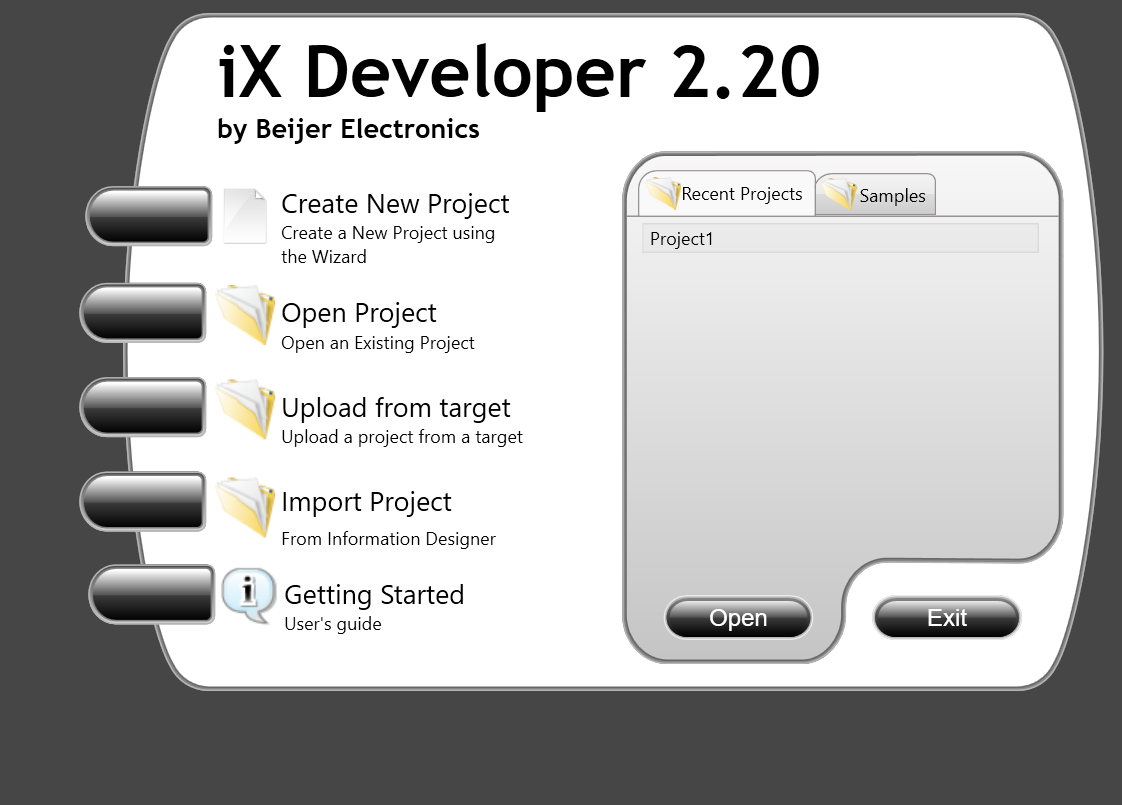
\includegraphics[width=8cm]
		{figuras/ix-new_project} 
		}}{ \Fonte{Elaborado pelo autor}    }
\end{figure}

Nesta tela inicial, algumas tarefas são possíveis, 
como abrir um projeto existente, 
ou mesmo consultar um guia de usuário. 
Para a criação de um novo projeto clique em 
\textit{\textbf{Create New Project}}.


A Figura \ref{fig:choose_target} 
ilustra a tela seguinte em que é necessário indicar o modelo de IHM que estamos utilizando. 


\begin{figure}[ht!]
	\centering
	\Caption{\label{fig:choose_target}Escolhendo um terminal gráfico }
	\UECEfig{}{\fbox{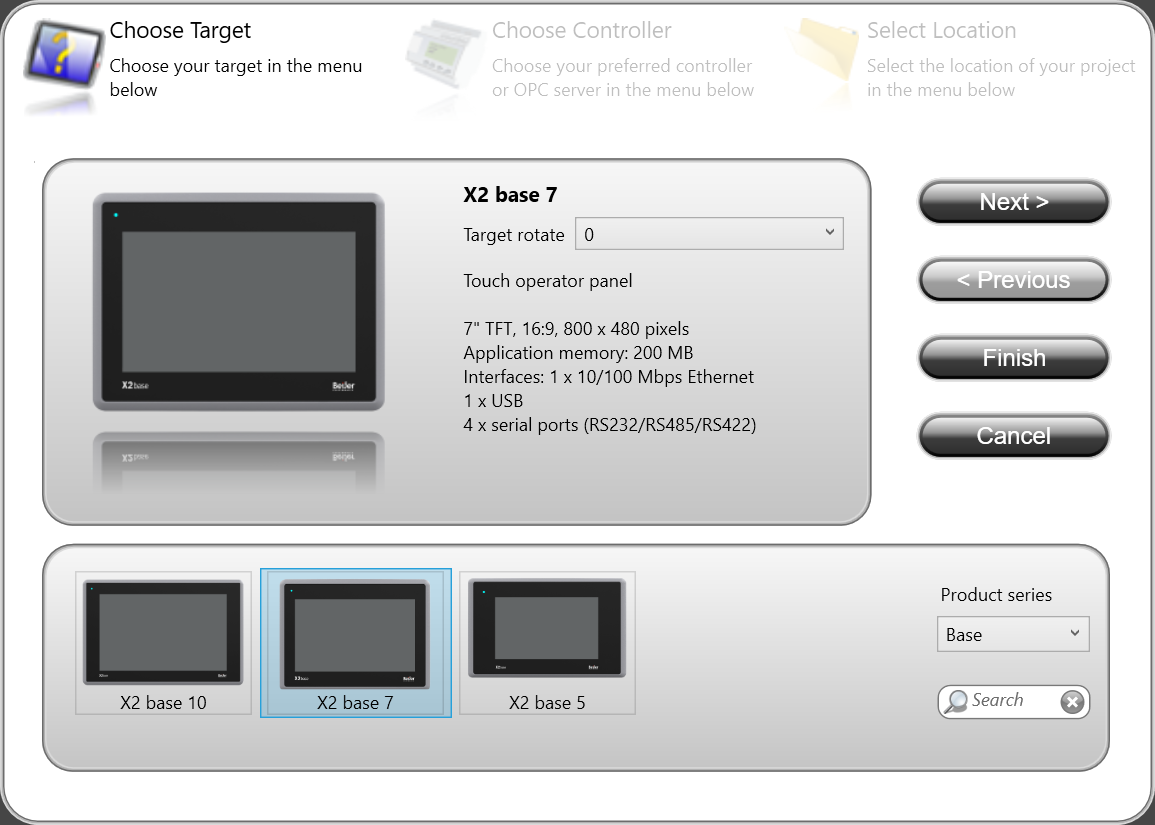
\includegraphics[width=8cm]
		{figuras/ix-choose_target } 
		}}{ \Fonte{Elaborado pelo autor}    }
\end{figure}


O modelo de terminal gráfico iX-T7F-2 foi descontinuado, 
e não há suporte no software, 
mas de acordo com a Notificação de Regime de Produção 
\cite{ix_t7f_2-x2_base_7} 
pode-se utilizar o modelo equivalente que é o 
\textbf{X2-BASE-7}, conforme selecionado na própria imagem.

Após a seleção do modelo, clique em \textbf{\textit{Next>}}.

A seleção seguinte é do controlador, que neste caso, 
significa escolher um protocolo de comunicação com a IHM. 

Selecione então \textbf{MODICON}, 
que é a desenvolvedora do protocolo Modbus, 
e deve ser selecionada na janela ao lado. 
Tomaremos a IHM como o \textbf{Cliente} da comunicação, 
então selecione \textbf{Modbus Master}.  



\begin{figure}[ht!]
	\centering
	\Caption{\label{fig:choose_controller}Escolhendo um protocolo de comunicação e uma marca de controlador}
	\UECEfig{}{\fbox{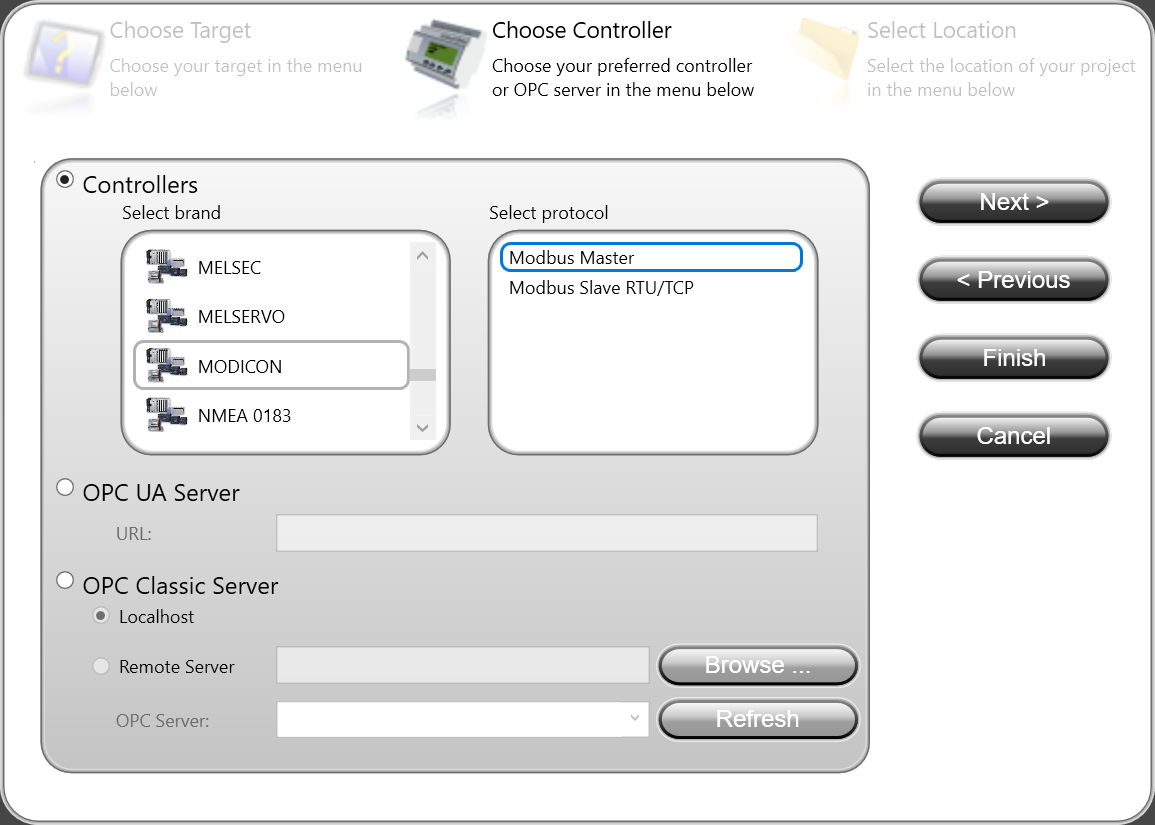
\includegraphics[width=8cm]
		{figuras/ix-choose_controller } 
		}}{ \Fonte{Elaborado pelo autor}    }
\end{figure}


Após a seleção do protocolo de comunicação, 
clique em \textbf{\textit{Next>}}.

A etapa final consiste na escolha de um local de armazenamento
e da escolha de um nome ao projeto, 
conforme Figura \ref{fig:select_location}.

\begin{figure}[ht!]
	\centering
	\Caption{\label{fig:select_location}Seleção de local de armazenamento do projeto }
	\UECEfig{}{\fbox{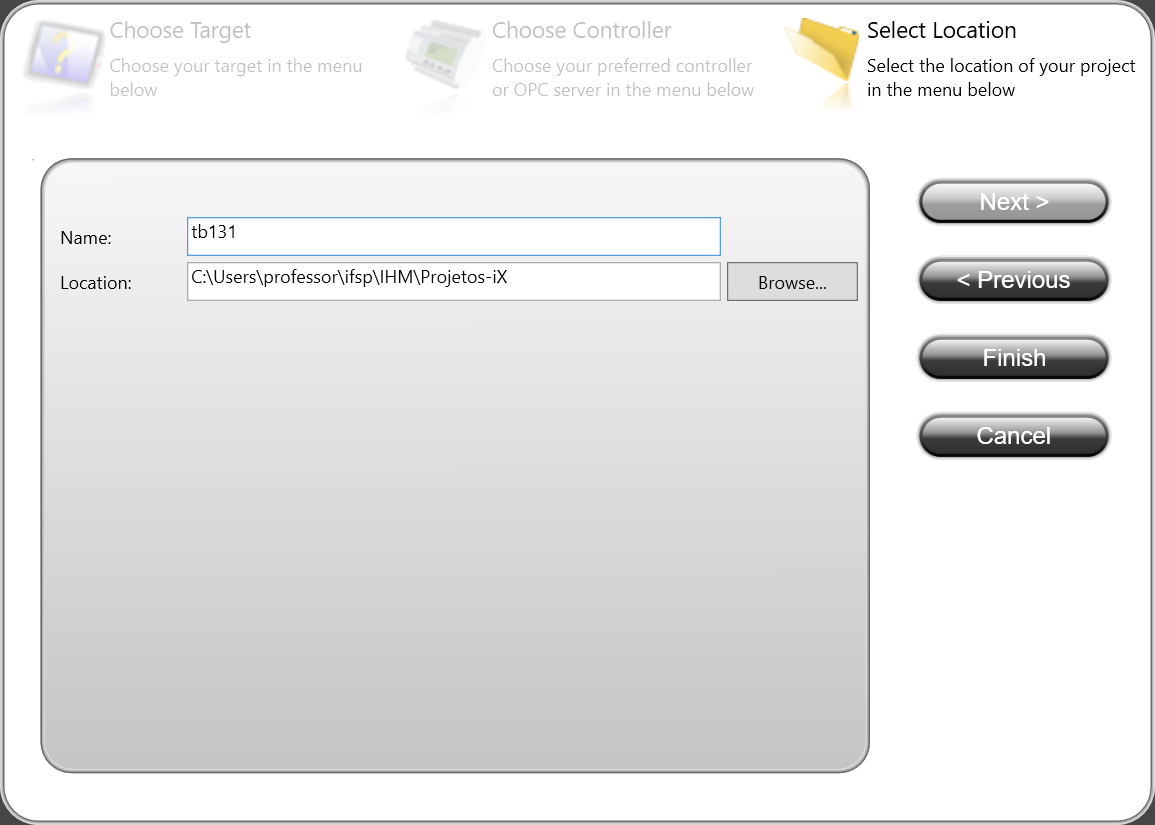
\includegraphics[width=8cm]
		{figuras/ix-select_location } 
		}}{ \Fonte{Elaborado pelo autor}    }
\end{figure}

Após a definição de local e nome do projeto 
clique em \textbf{\textit{Finish}}.

A Figura \ref{fig:screen1} 
ilustra a tela inicial para a criação de um projeto. 


\begin{figure}[ht!]
	\centering
	\Caption{\label{fig:screen1}Tela inicial ao criar um novo projeto}
	\UECEfig{}{\fbox{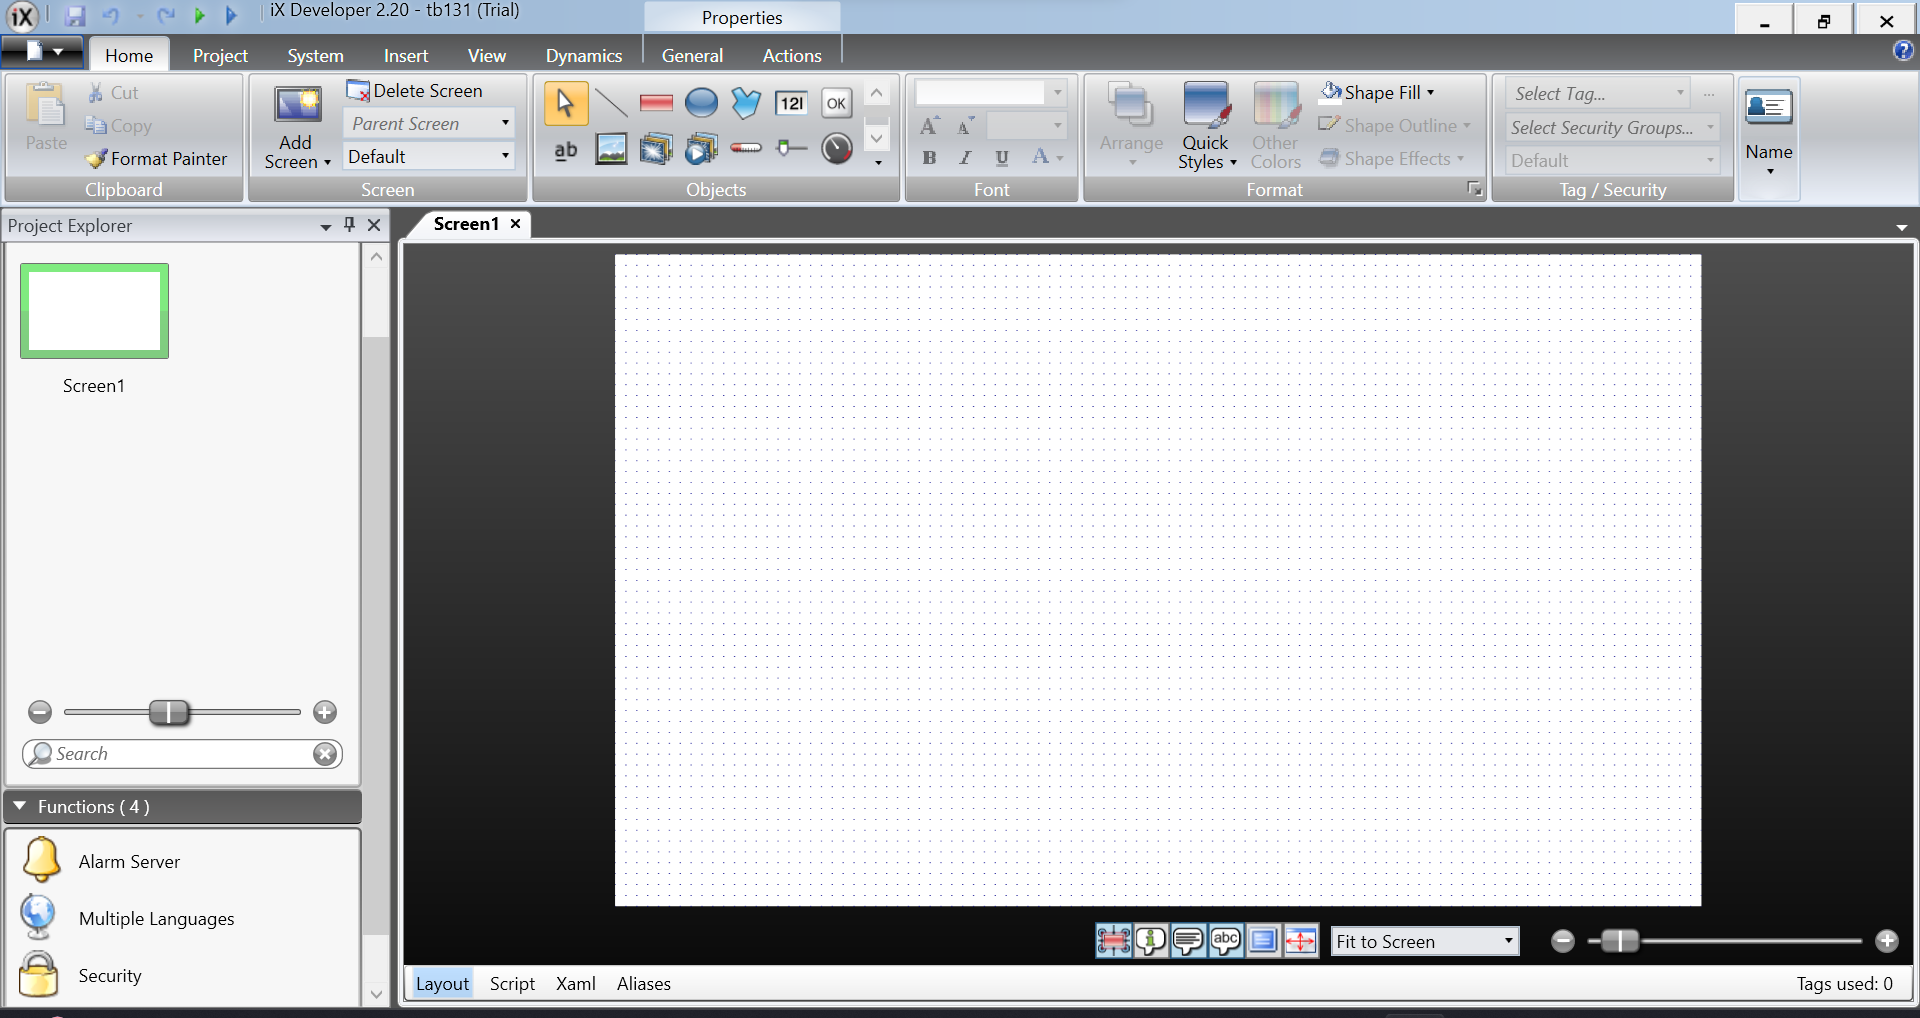
\includegraphics[width=14cm]
		{figuras/ix-screen1} 
		}}{ \Fonte{Elaborado pelo autor}    }
\end{figure}





\section{Configurando TAGs}


Após a criação do projeto, 
recomenda-se iniciar pela declaração de TAGs, 
que são as variáveis, que conectam os elementos gráficos com as respectivas variáveis do controlador. 

A Figura \ref{fig:functions-tags} 
ilustra a sequência de passos para a declaração das TAGs. 
Ao clicar na opção \textbf{Tags} 
no quadro \textbf{Functions}, 
\textbf{indicador 1}, 
na tela principal abre-se uma aba para a declaração das Tags, 
\textbf{indicador 2}.



\begin{figure}[ht!]
	\centering
	\Caption{\label{fig:functions-tags} Incluindo TAGs ao projeto }
	\UECEfig{}{\fbox{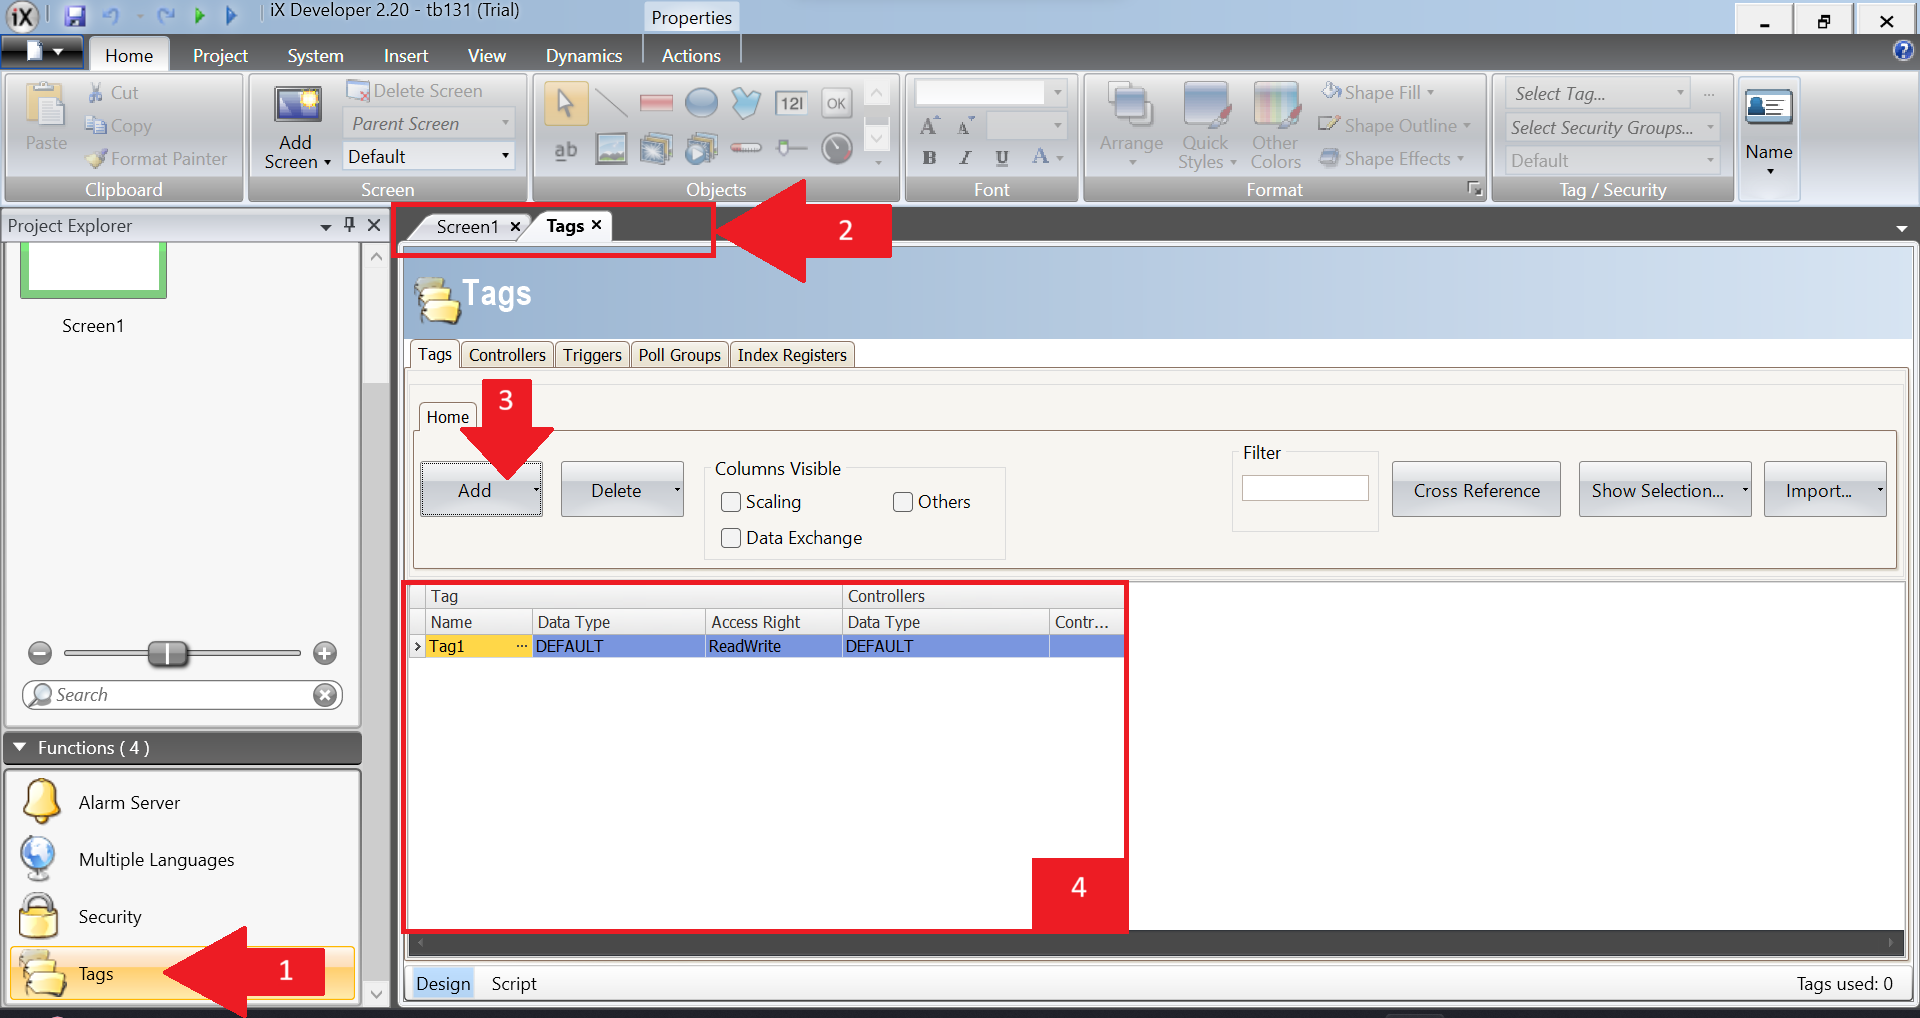
\includegraphics[width=14cm]
		{figuras/ix-functions-tags-n } 
		}}{ \Fonte{Elaborado pelo autor}    }
\end{figure}



Clicando em \textbf{Add}, \textbf{indicador 3}, 
são adicionadas TAGs no quadro do \textbf{indicador 4}. 
Todas as variáveis do controlador que forem ser representadas ou manipuladas de alguma forma, devem ser declaradas como TAGs. 


A Figura \ref{fig:tags} 
ilustra as TAGs envolvidas no projeto para a comunicação com o TB131. 
O conjunto de TAGs possui três propriedades, 
\textbf{Nome}, \textbf{Tipo de Dado} e \textbf{Direito de Acesso}.
De forma correlata, 
cada TAG possui um respectivo endereço Modbus e seu tipo. 



\begin{figure}[ht!]
	\centering
	\Caption{\label{fig:tags} As Tags do projeto }
	\UECEfig{}{\fbox{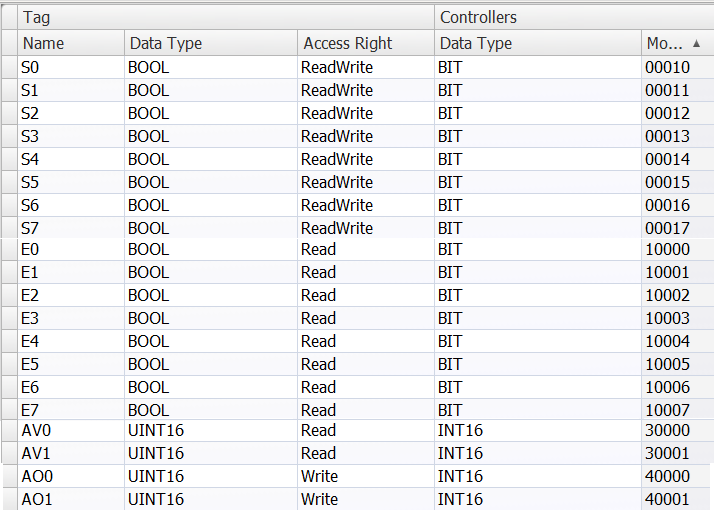
\includegraphics[width=10cm]
		{figuras/ix-tags-n } 
		}}{ \Fonte{Elaborado pelo autor}    }
\end{figure}


As variáveis de saída do TB131 
são ligados às variáveis nomeadas de S0 a S7, 
do tipo Booleana e com direito de acesso a leitura e escrita. 
Os endereços Modbus são associados às funções, 
representados em hexadecimal com os valores de 00010h até 00017h,
para acesso às \textit{Coils}, ou seja, as saídas digitais ou bobinas no CLP. 

As variáveis de entrada do TB131 
são ligadas às variáveis nomeadas de E0 até E7, 
do tipo Booleana e com direito de acesso somente a leitura. 
Os endereço Modbus estão no intervalo 10000h até 10007h, 
para Discrete Inputs, ou seja, as entradas digitais.

As variáveis AV0 e AV1 
são conectadas aos valores analógicos dos potenciômetros do TB131,
do tipo UINT16, inteiro de 16bits sem sinal, somente leitura. 
São endereçadas entre 30000h e 30001h. 

As variáveis AO0 e AO1 
são conectadas aos valores analógicos de saída do TB131, 
do tipo UINT16, interiro de 16bits sem sinal, somente escrita. 
São endereçadas em 40000h e 40001h. 



\begin{figure}[ht!]
	\centering
	\Caption{\label{fig:controller_settings} Parâmetros do controlador }
	\UECEfig{}{\fbox{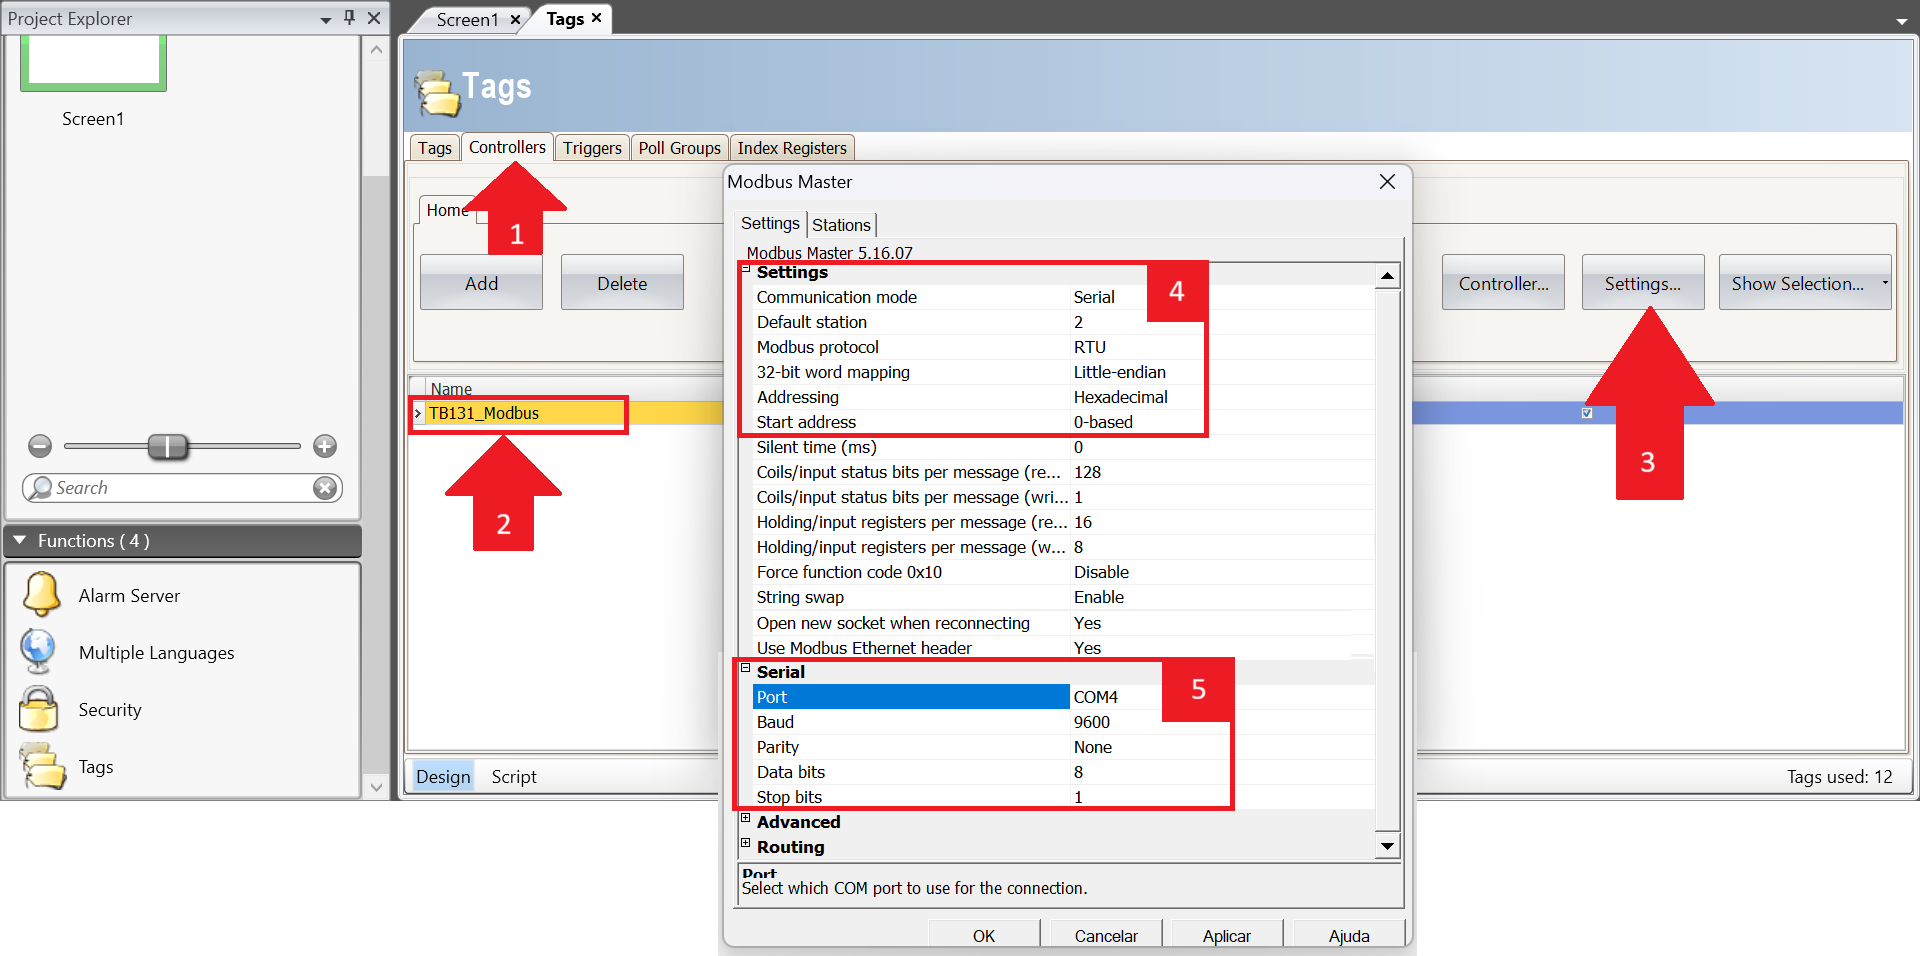
\includegraphics[width=14cm]
		{figuras/ix-controller_settings-n } 
		}}{ \Fonte{Elaborado pelo autor}    }
\end{figure}




A Figura \ref{fig:controller_settings} ilustra 
os passos da configuração da comunicação com o controlador, 
clicando no \textbf{indicador 1}.
No \textbf{indicador 2}, 
pode-se renomear o controlador, 
principalmente se houverem outros controladores envolvidos do processo. 



Clicando no \textbf{indicador 3}, 
podem ser configurados os parâmetros da comunicação Modbus, 
no \textbf{indicador 4} e da porta serial no \textbf{indicador 5}.


Além desta configuração e escolha de porta (COM2 ou COM4), 
é necessário habilitar a porta de comunicação serial que será utilizada conforme Figura \ref{fig:serial_port}. 


\begin{figure}[ht!]
	\centering
	\Caption{\label{fig:serial_port} Configurando porta de comunicação para RS485 }
	\UECEfig{}{\fbox{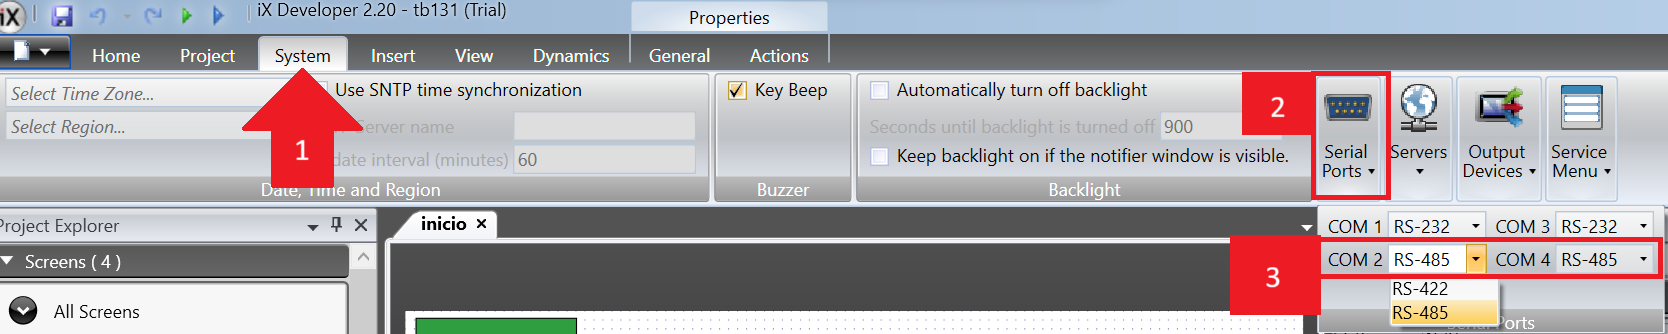
\includegraphics[width=12cm]
		{figuras/ix-serial_port-n } 
		}}{ \Fonte{Elaborado pelo autor}    }
\end{figure}

%As portas de comunicação COM1 e COM2 
%compartilham um mesmo conector, assim como COM3 e COM4. 

As portas COM2 e COM4 podem ser configuradas como RS-485 e RS-422.
No caso deste projeto, selecione a RS-485 de acordo com a porta COM selecionada anteriormente. 





\section{Inclusão de objetos gráficos}


A montagem das telas, 
basicamente acontece inserindo os elementos denominados objetos, 
que podem ser desde formas simples até indicadores com animação. 


A Figura \ref{fig:obj_properties} 
ilustra a inserção de objetos formando a primeira tela do projeto,
composta pelo logo do IFSP e de uma barra lateral na cor verde.



\begin{figure}[ht!]
	\centering
	\Caption{\label{fig:obj_properties} Propriedade dos objetos  }
	\UECEfig{}{\fbox{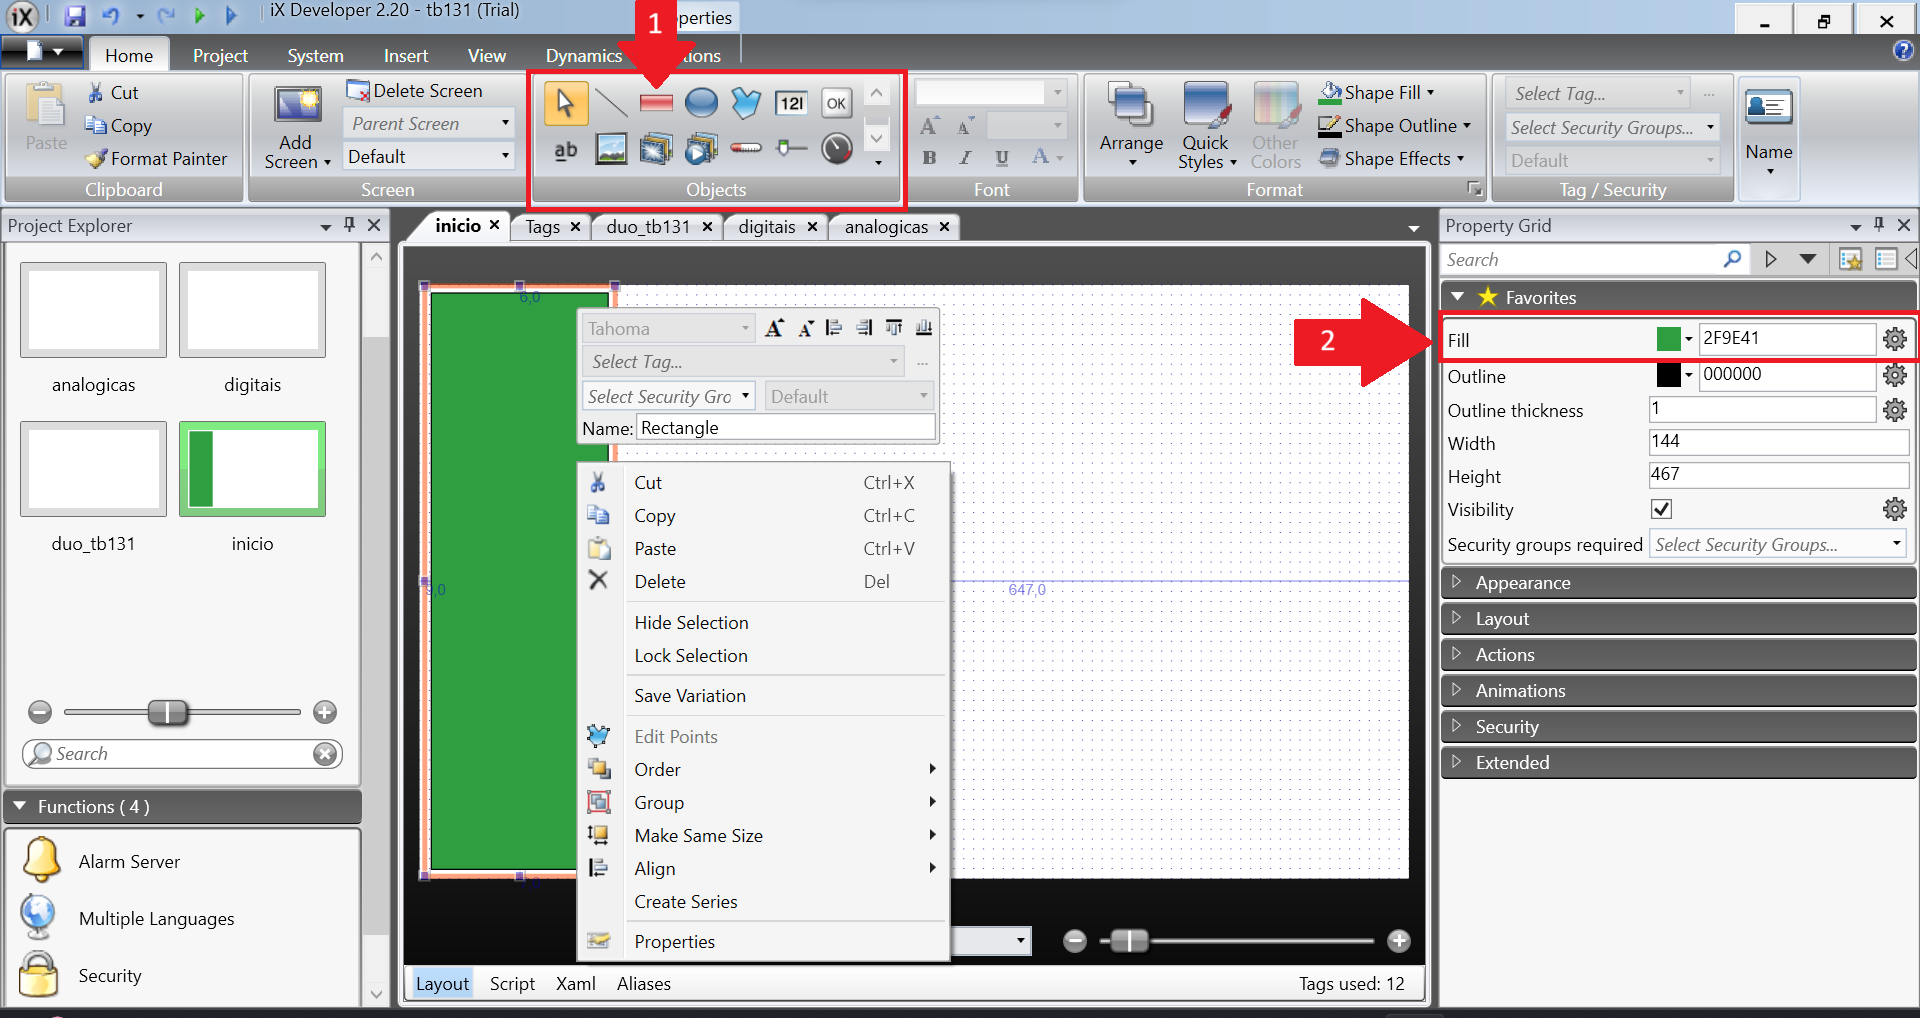
\includegraphics[width=12cm]
		{figuras/ix-objects_properties-n}
		}}{ \Fonte{Elaborado pelo autor}    }
\end{figure}


O \textbf{indicador 1} aponta o objeto utilizado, 
que é a forma retungular.
Ao cliacar com \textbf{botão direito do mouse} sobre a forma inserida, 
a opção \textit{\textbf{Properties}}, 
abre uma janela lateral com as propriedades do objeto. 

O \textbf{indicador 2} 
aponta a propriedade de cor do preenchimento, 
que está ajustada no formato RGB hexadecimal com o valor \textbf{2F9E41h}, 
que é a cor verde oficial do logo do IFSP.

Outros parâmetros podem ser ajustados a depender do visual que se queira obter. Explore!


A Figura \ref{fig:tela_inicio} 
ilustra os passos para a inserção de uma imagem externa como elemento visual da tela. 
Ao clicar no ícone, deve-se marcar um quadro na tela, 
na posição em que a imagem será inserida.
Ao fazer isso, 
abre-se uma janela de busca, 
padrão do sistema operacional, 
da mesma forma que ocorre ao salvar um arquivo. 
Após a seleção do elemento, 
ele é inserido no quadro marcado inicialmente. 
Após a inserção é possivel redimensionar o tamanho da imagem, dentre outas propriedades possíveis de edição.

\begin{figure}[ht!]
	\centering
	\Caption{\label{fig:tela_inicio} Adicionando imagem externa em uma tela }
	\UECEfig{}{\fbox{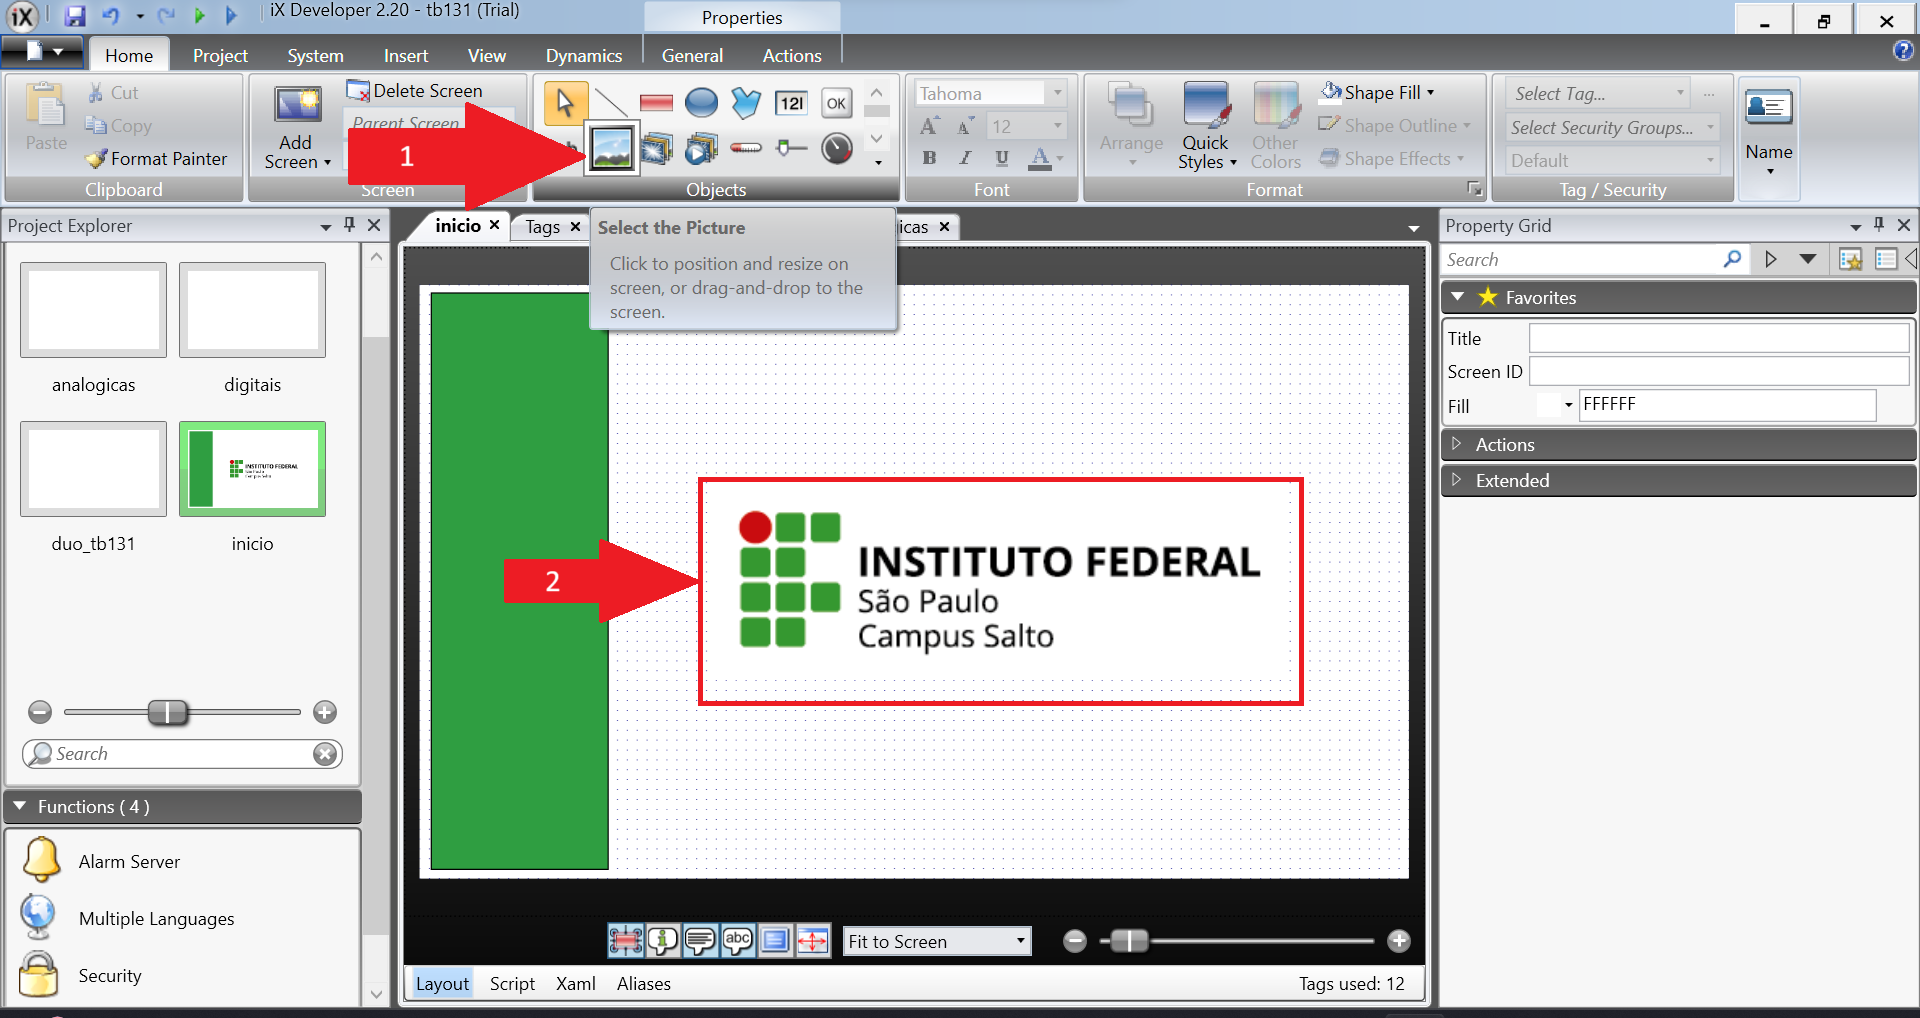
\includegraphics[width=14cm]
		{figuras/ix-tela_inicio-n}
		}}{ \Fonte{Elaborado pelo autor}    }
\end{figure}

Para a atribuição de ação ao objeto inserido na tela, 
ilustrado na Figura \ref{fig:screen_inicio},
é possivel definir que tipo de evento irá produzir a ação, 
na janela de propriedades, seção \textbf{\textit{Actions}}.



\begin{figure}[ht!]
	\centering
	\Caption{\label{fig:screen_inicio} Configurando evendo de transição de tela }
	\UECEfig{}{\fbox{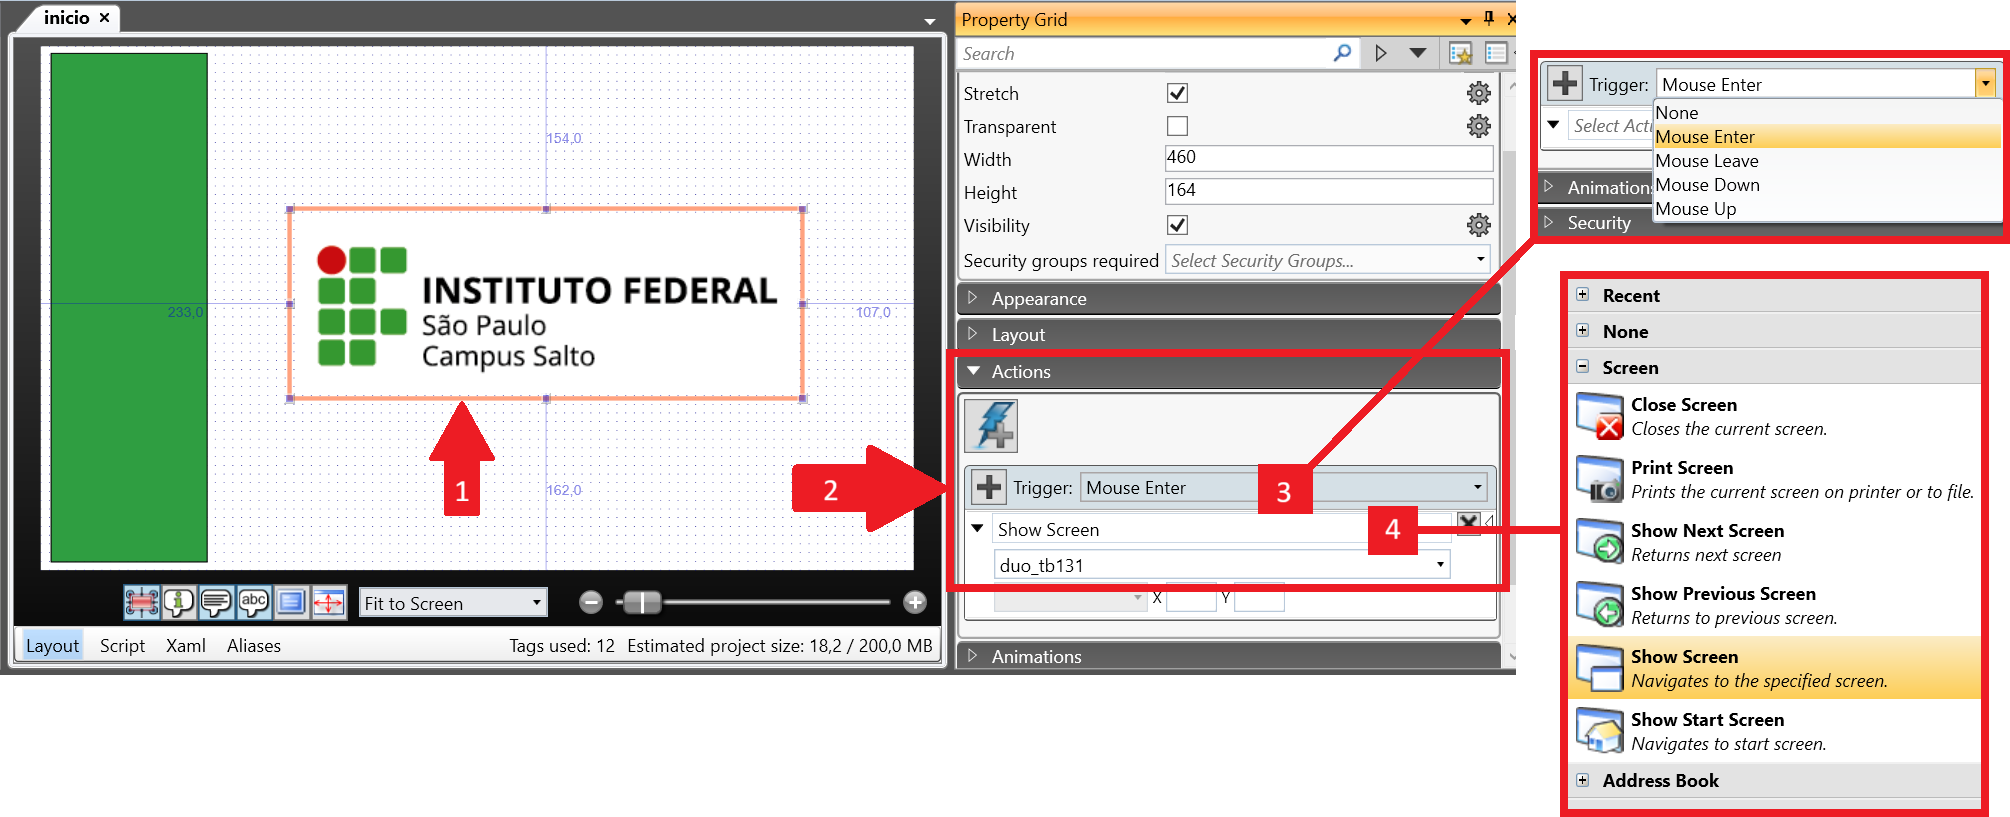
\includegraphics[width=15cm]
		{figuras/ix-screen_inicio-n}
		}}{ \Fonte{Elaborado pelo autor}    }
\end{figure}


O evendo selecionado no \textbf{indicador 3}, 
foi um \textbf{clique do mouse} no objeto, 
que dispara a ação correspondente, 
que é a transição de tela, 
conforme \textbf{indicador 4}, 
cujo último parâmetro do \textbf{indicador 2}, 
é a tela de destino. 



A Figura \ref{fig:select_polyline} 
evidencia a ferramenta denominada \textbf{Poly Line} 
que permite a produção de formas distintas às básicas, 
retangulares e circulares. 
Os trapézios retangulares utilizados como botões de transição 
às respectivas telas foram feitos utilizando esta ferramenta. 


\begin{figure}[ht!]
	\centering
	\Caption{\label{fig:select_polyline} Botões do menu principal }
	\UECEfig{}{\fbox{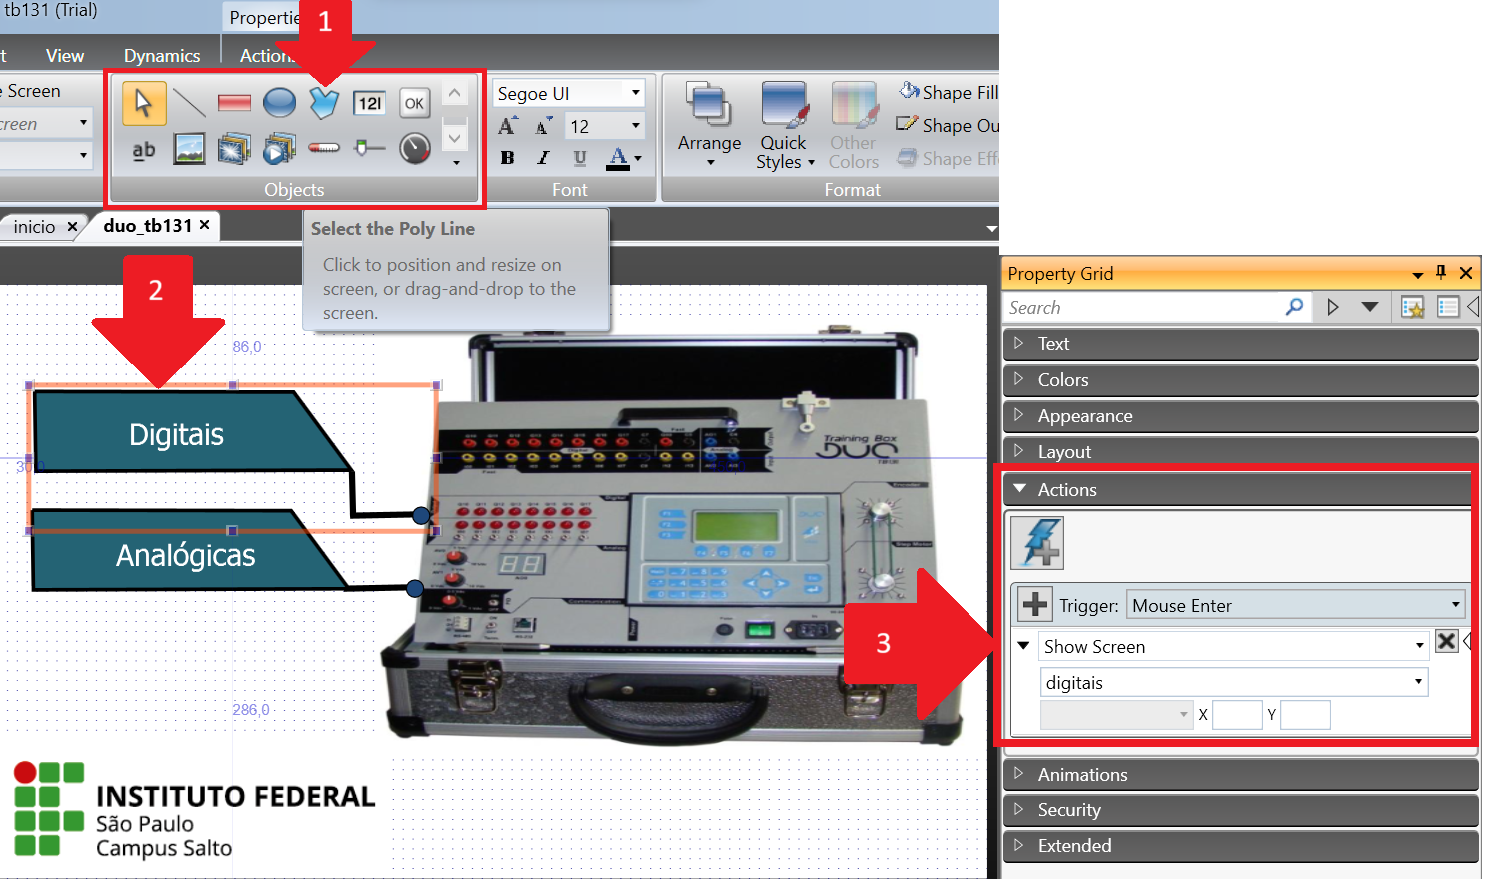
\includegraphics[width=14cm]
		{figuras/ix-screen-select_polyline-n}
		}}{ \Fonte{Elaborado pelo autor}    }
\end{figure}

A produção da transição da tela de menu para a tela das 
entradas e saídas digitais é feita de forma análoga à 
transição da tela inical. 



As entradas digitais, 
são representadas com circulos conforme 
\textbf{indicador 1} da Figura 
\ref{fig:digitais_entradas}, 
sendo um elemento com duas cores 
a depender do estado lógico da respectiva variável que este elemento representa. 

\begin{figure}[ht!]
	\centering
	\Caption{\label{fig:digitais_entradas} Configuração dos sinalizadores das entradas digitais }
	\UECEfig{}{\fbox{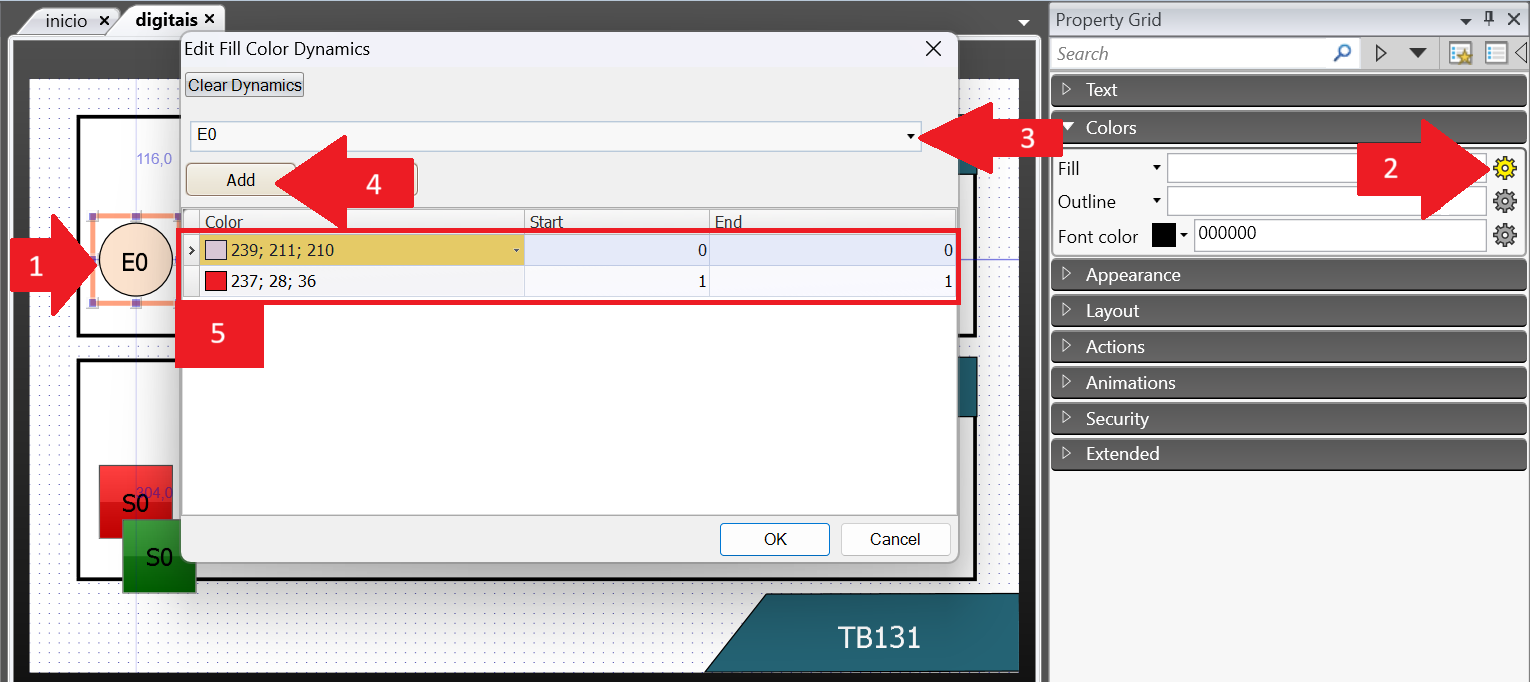
\includegraphics[width=14cm]
		{figuras/ix-digitais_entradas_fillcolor-n}
		}}{ \Fonte{Elaborado pelo autor}    }
\end{figure}

Acessando as propriedades do objeto, 
e clicando na engrenagem correspondente ao 
campo de preenchimento de cor, 
\textbf{indicador 2}, 
pode-se configurar uma variável para associar este objeto,
\textbf{indicador 3}, 
e adicionar uma cor,
\textbf{indicador 4} 
para cada estado lógico da variável,
\textbf{indicador 5}.



As saídas digitais possuem um efeito de 
ao pressionar o botão, 
mudar o estado lógico da variável e 
mudar a própria cor do botão, 
porém este efeito foi produzido utilizando 
dois botões de cor única, 
alternando a propriedade de visibilidade.


A Figura \ref{fig:digitais_saidas} 
ilustra a configuração para o botão desligar, 
na cor vermelha, 
mas o processo é o mesmo para o botão verde, 
exceto pelo estado que produz a visibilidade do objeto.


\begin{figure}[ht!]
	\centering
	\Caption{\label{fig:digitais_saidas} Configuração dos sinalizadores das saídas digitais}
	\UECEfig{}{\fbox{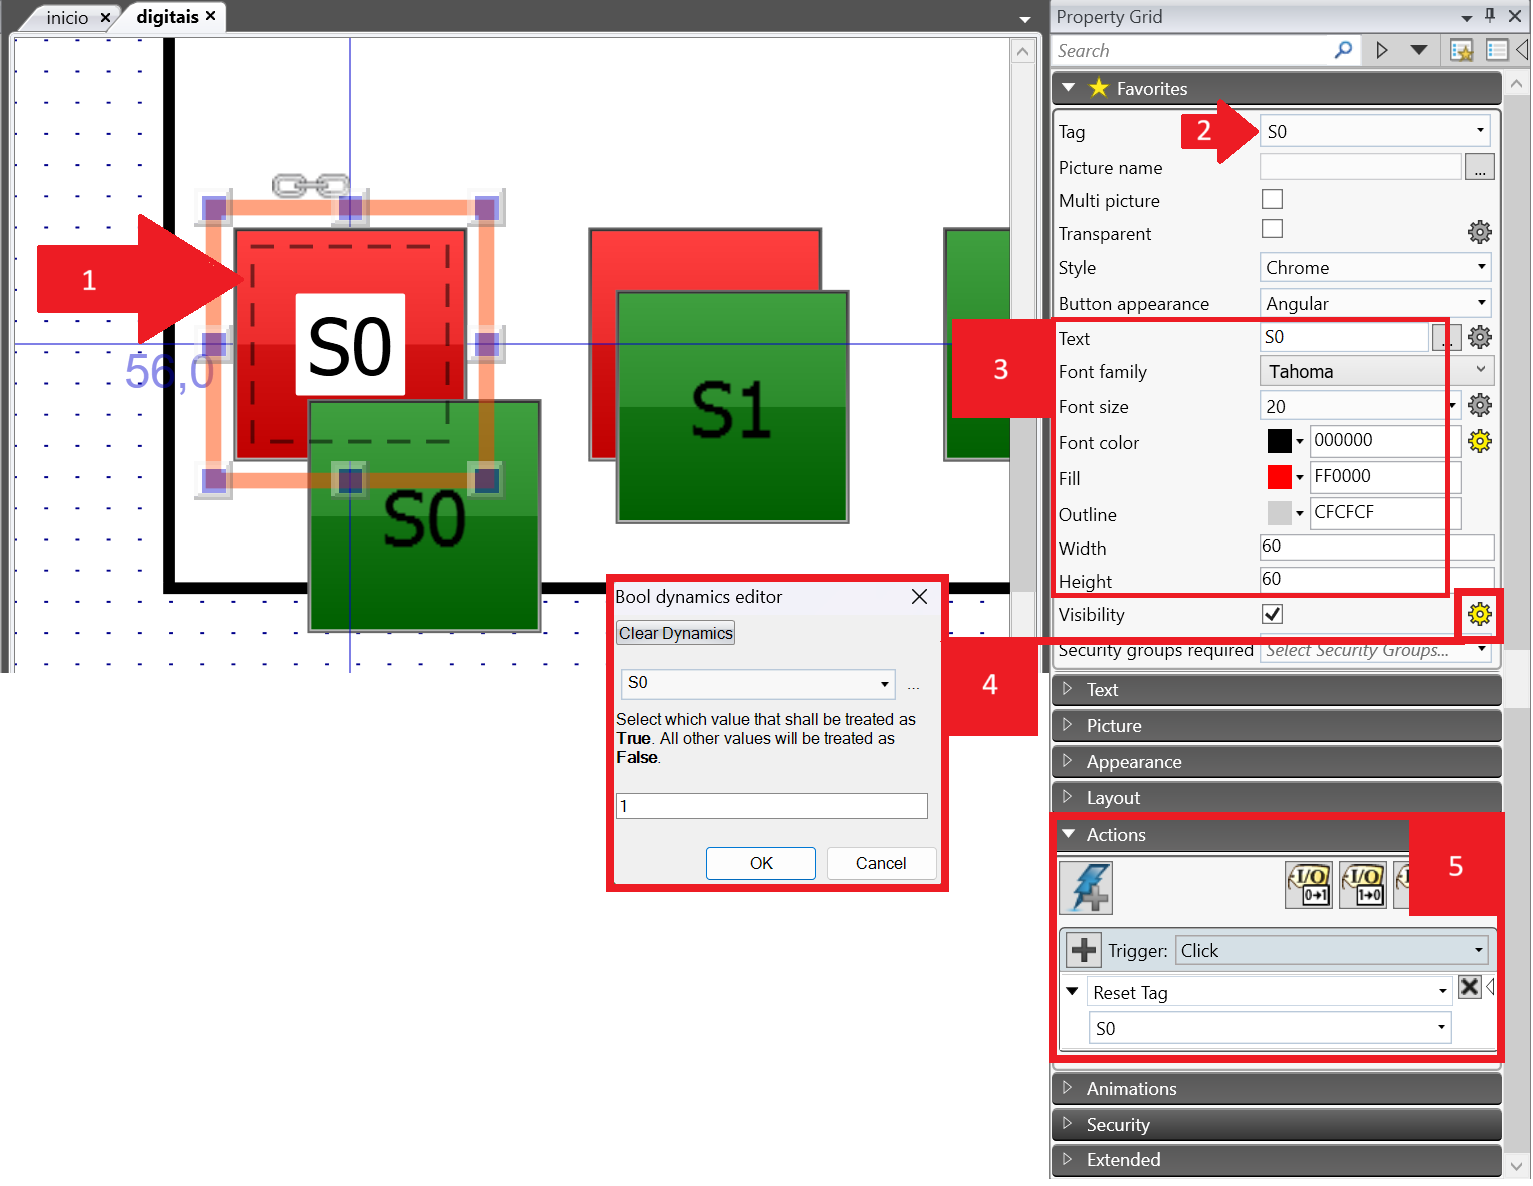
\includegraphics[width=14cm]
		{figuras/ix-digitais_saidas_vermelho-n}
		}}{ \Fonte{Elaborado pelo autor}    }
\end{figure}


O passo inicial consiste em abrir as propriedades do objeto,
\textbf{indicador 1}. 

Indicar a TAG associada ao objeto,
\textbf{indicador 2}.

Ajustar os parâmetros visuais,
\textbf{indicador 3},
como texto exibido, cor, tamanho de fonte, e dimensões do objeto.

Acessando as configurações da opção de visibilidade,
(\textbf{\textit{Visibility}}), 
deve-se novamente apontar a TAG que servirá de referência,
\textbf{indicador 4},
e qual o seu valor que condiciona a visibilidade do objeto. 
Neste caso, 
quando a variável \textbf{S0} 
possuir o valor lógico \textbf{1}, 
significa que a saída está ligada, 
e o botão vermelho irá ficar visível para uma futura ação de desligar. 

Por fim, a ação associada ao objeto,
\textbf{indicador 5},
é o \textbf{reset Tag} de \textbf{S0}, 
produzido pelo \textbf{click} no objeto.


Para o botão verde, 
os parâmetros são os mesmos, 
exceto a cor do botão e o 
estado da TAG que torna o objeto visível, 
que neste caso é o valor lógico 0.






Para as variáveis analógicas, 
são utilizados objetos de controle para a interface, 
como medidores analógicos, lineares, circulares e slider, 
destacados na Figura \ref{fig:analog_obj}.




\begin{figure}[ht!]
	\centering
	\Caption{\label{fig:analog_obj} Elementos gráficos de controle }
	\UECEfig{}{\fbox{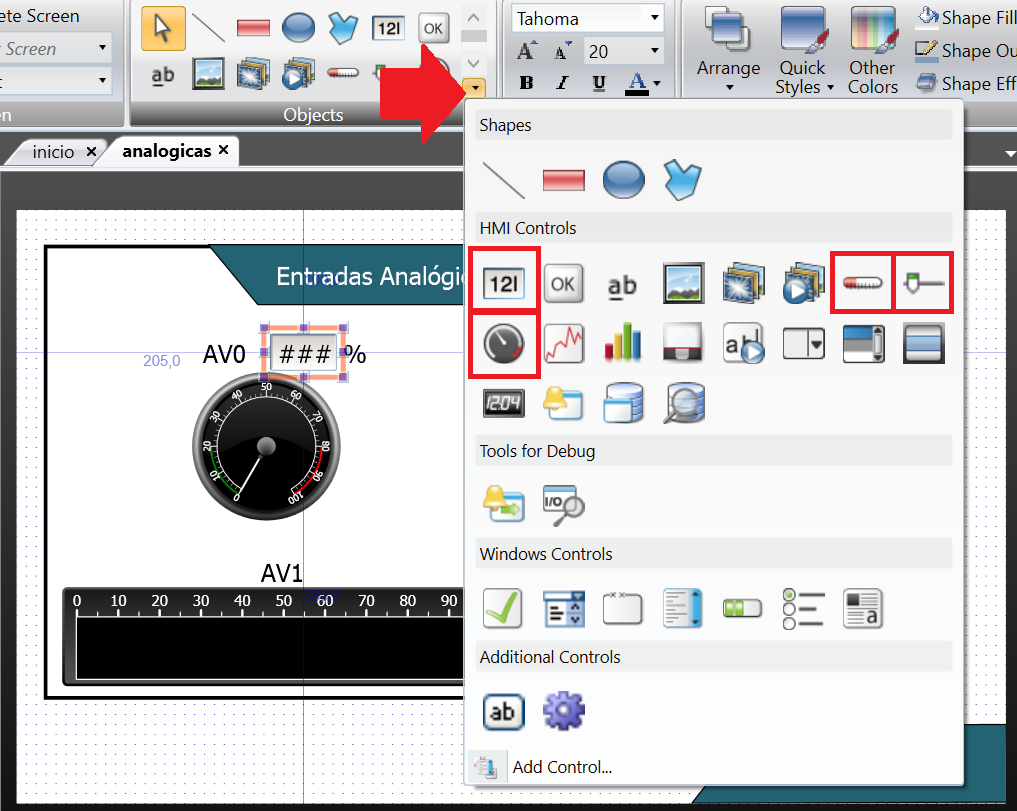
\includegraphics[width=14cm]
		{figuras/ix-analogicos_objects-n}
		}}{ \Fonte{Elaborado pelo autor}    }
\end{figure}




O mostrador analógico é um dos elementos mais simples e m
ais utilizados, inclusive, 
e alguns de seus parâmetros estão destacados na 
Figura \ref{fig:analog_meter}, 
como o apontamento da TAG que servirá de referência e
o formato do dado exibido. 
No segundo destaque o fato de ser um elemento somente de leitura,
impedindo a edição do valor exibido. 
O último destaque para o tamanho da fonte. 
Outras propriedades podem ser alteradas dependendo da necessidade funcional ou estética. 
Explore!


\begin{figure}[ht!]
	\centering
	\Caption{\label{fig:analog_meter} Mostrador analógico }
	\UECEfig{}{\fbox{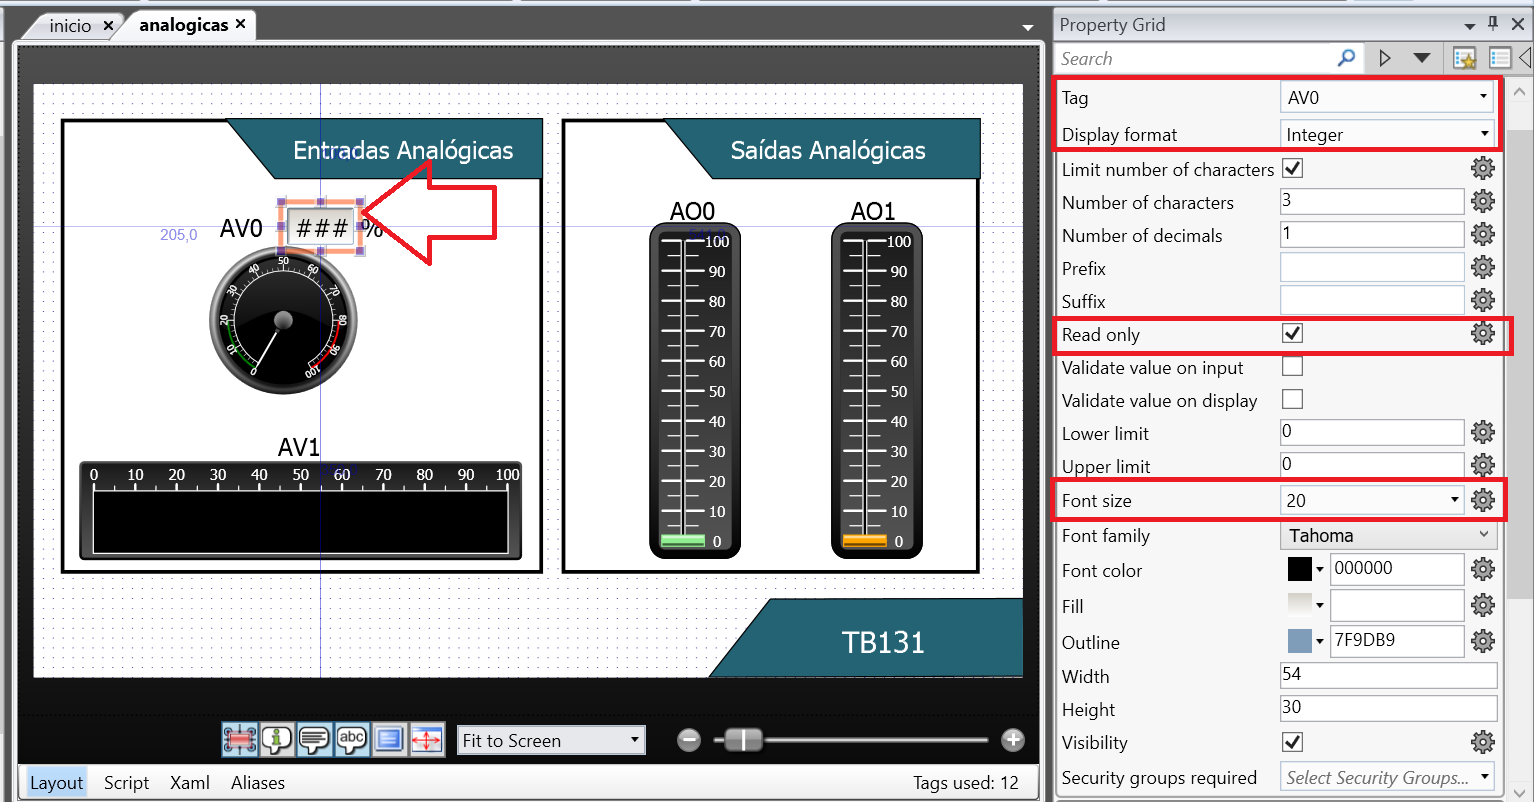
\includegraphics[width=14cm]
		{figuras/ix-analogicos_analogmeter-n}
		}}{ \Fonte{Elaborado pelo autor}    }
\end{figure}





O mostrador circular é 
o mostrador símbolo de variáveis analógicas
(mesmo que transmitidas por uma canal digital). 
A Figura \ref{fig:analog_circularmeter} 
destaca algus parâmetros dentre os muitos possíveis. 
No destaque superior é apontada a TAG de referência e 
os valores extremos de exibição. 
O destaque seguinte, 
o tipo de mostrador e o tamanho da fonte. 
O destaque inferior mostra as dimensões do objeto. 




\begin{figure}[ht!]
	\centering
	\Caption{\label{fig:analog_circularmeter} Mostrador circular }
	\UECEfig{}{\fbox{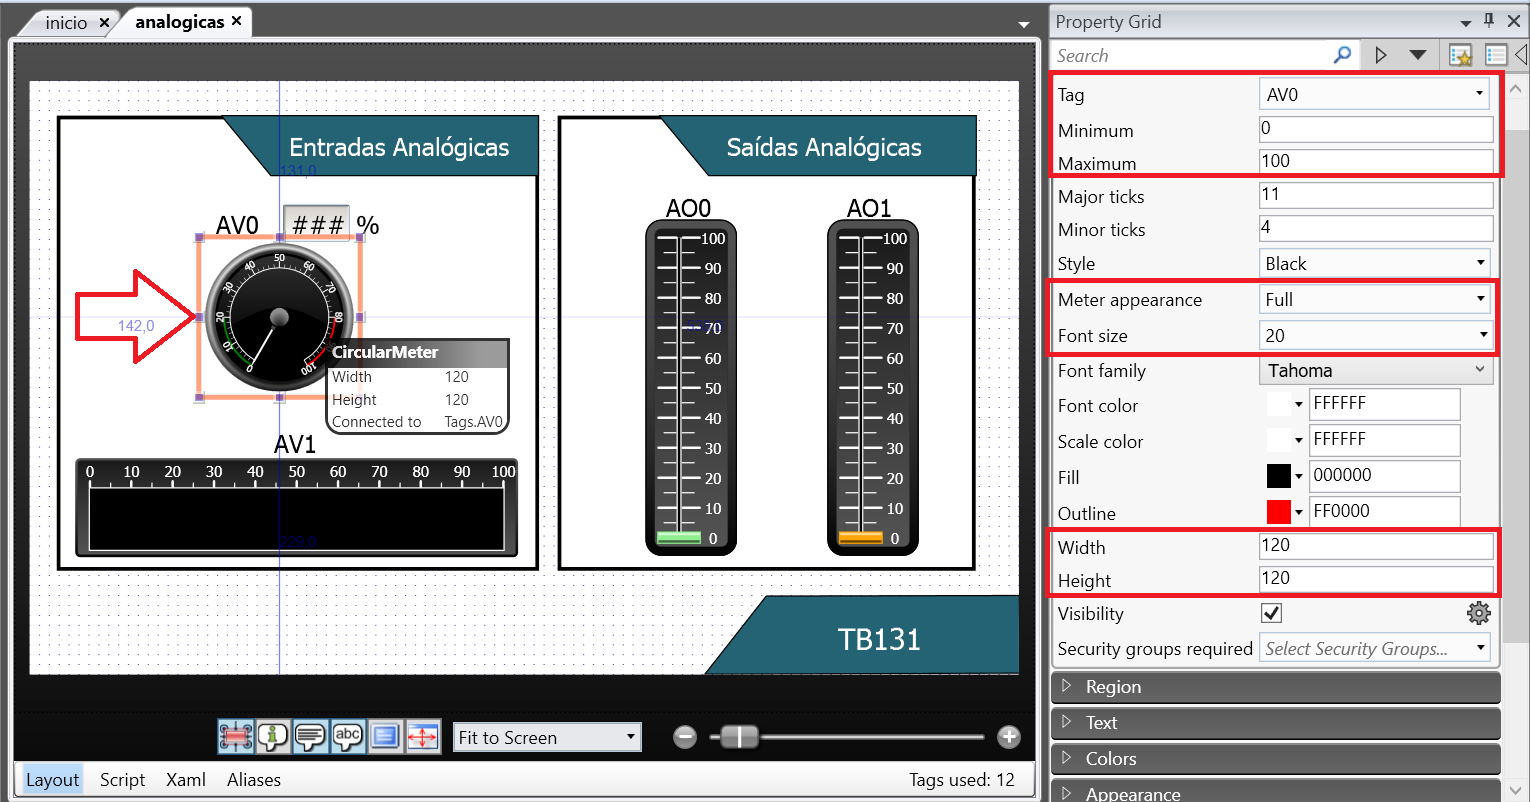
\includegraphics[width=14cm]
		{figuras/ix-analogicos_circularmeter-n}
		}}{ \Fonte{Elaborado pelo autor}    }
\end{figure}




O mostrador linear, 
possui parâmetros semelhantes ao circular,
\textbf{indicador 2},
como o apontamento da TAG de referência e os extremos de exibição,
valor máximo e valor mínimo. 


\begin{figure}[ht!]
	\centering
	\Caption{\label{fig:analog_linearmeter} Mostrador Linear }
	\UECEfig{}{\fbox{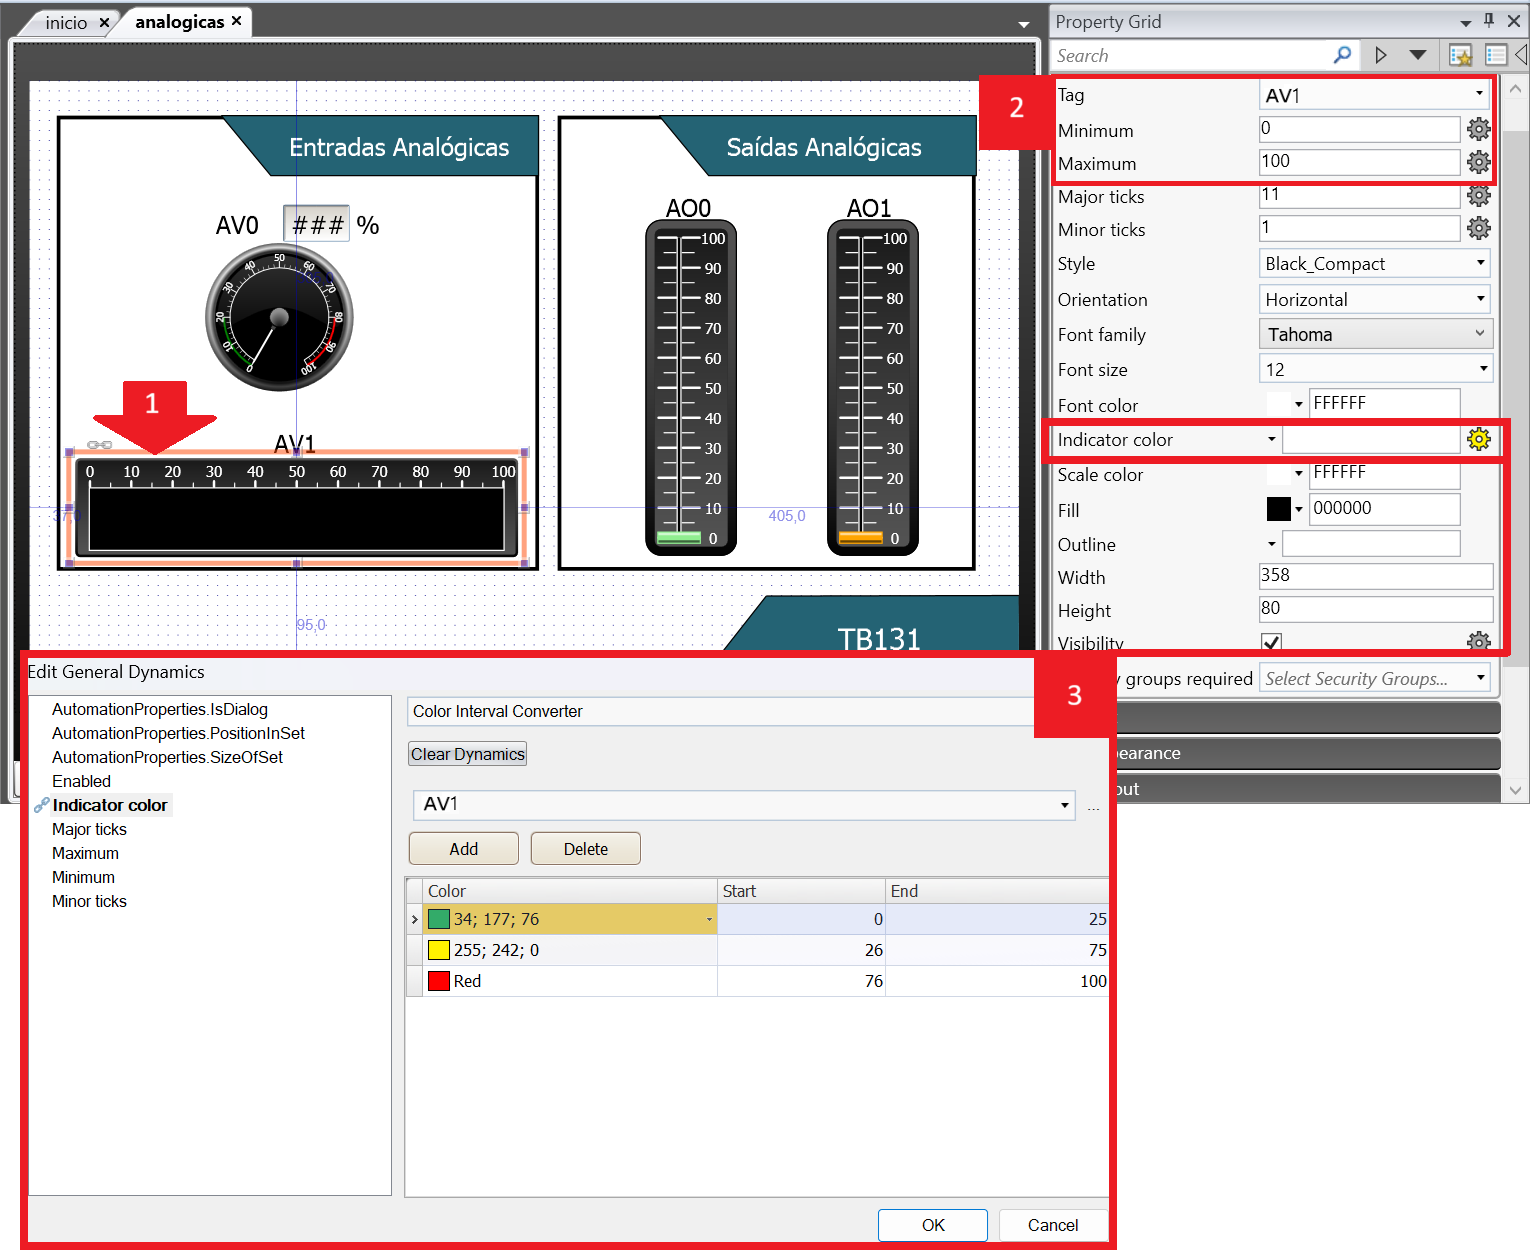
\includegraphics[width=14cm]
		{figuras/ix-analogicos_linearmeter-n}
		}}{ \Fonte{Elaborado pelo autor}    }
\end{figure}

Porém, neste caso é possível mudar a cor da barra de progresso 
a depender do valor da variável analógica de referência. 
Acessando as configurações do parâmetro 
\textbf{\textit{Indicator color}},
\textbf{indicador 3}, 
deve-se novamente indicar a TAG de referência e 
adicionar intervalos com as respectivas cores. 
O exemplo mostra a utilização de três intervalos com três respectivas cores.



Como elemento de atuação nas variáveis analógicas, 
é utilizado a objeto denominado \textbf{slider}, 
cujas propriedades são destacadas na 
Figura \ref{fig:analog_slider}. 
Assim como os demais elementos, 
deve-se apontar a TAG que servirá de referência para 
a manipulação dos dados,
\textbf{indicador 2}, 
bem como seus valores extremos.

Podem ser alterados diversos parâmetros, 
novamente, a depender da necessidade técnica ou visual, 
como a cor do elemento cursor, 
\textbf{indicador 3}. 




\begin{figure}[ht!]
	\centering
	\Caption{\label{fig:analog_slider} Chave deslizante }
	\UECEfig{}{\fbox{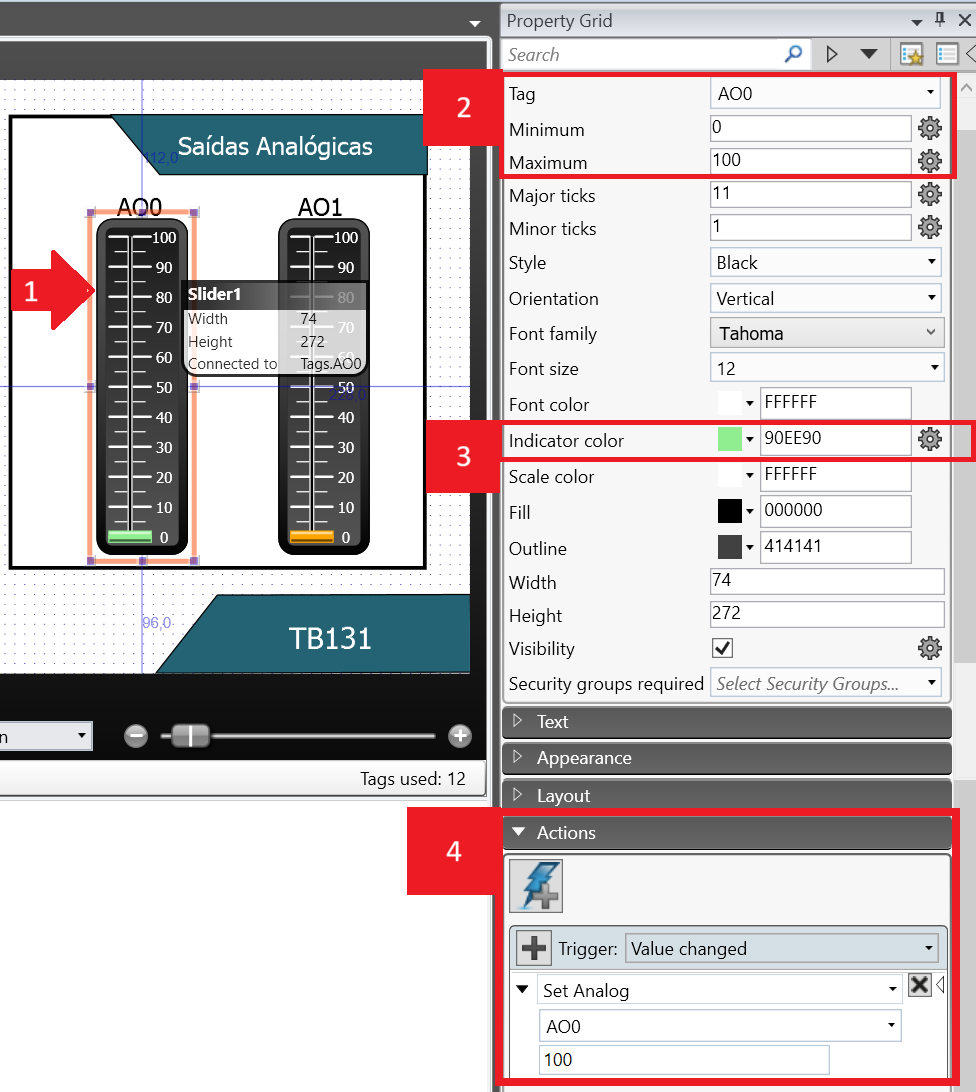
\includegraphics[width=14cm]
		{figuras/ix-analogicos_slider-n}
		}}{ \Fonte{Elaborado pelo autor}    }
\end{figure}




O parâmetro mais importante no caso de um elemento de atuação, 
é a sua configuração de ação,
\textbf{indicador 4},
em que para uma mudança de valor no seu cursor, 
ocorre a ação, 
\textbf{\textit{Set Analog}}, 
na TAG apontada e com o fundo de escala definido abaixo, 
que neste exemplo a TAG é a \textbf{AO0} 
e o fundo de escala é \textbf{100}. 


Desta forma, 
são realizadas as configurações básicas dos elementos gráficos, 
ou objetos, contidos na tela e que fazem 
a interface dos dados mediante a comunicação com o controlador.





\section{Tranferindo o projeto para o Terminal Gráfico/IHM}


Ao finalizar o desenvolimento de uma etapa do projeto, 
não somente ao final dele, 
recomenda-se que seja realizada a construção do projeto 
(\textbf{\textit{build}}), 
que consiste basicamente da compilação do que foi configurado até então, 
produzindo um arquivo executável a ser transferido ao equipamento. 

Este processo permite 
a detecção de erros de construção no projeto, 
de modo que sejam detectados o quanto antes e corrigidos.

Para este processo, 
acesse a opção \textbf{\textit{project}}, 
como na Figura \ref{fig:project_build} e 
clique em \textbf{\textit{build}},
\textbf{indicador 1}.



\begin{figure}[ht!]
	\centering
	\Caption{\label{fig:project_build} Compilação e download do projeto }
	\UECEfig{}{\fbox{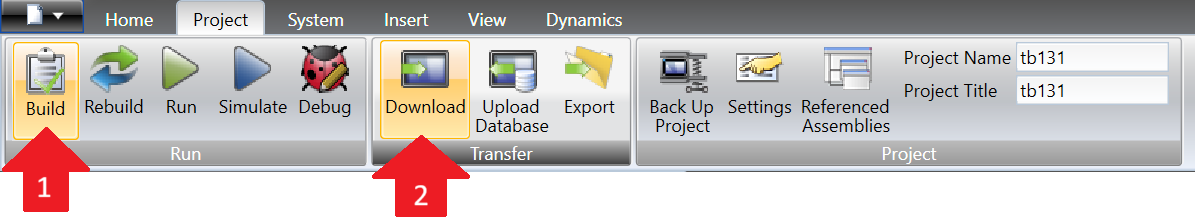
\includegraphics[width=14cm]
		{figuras/ix-project_download-n}
		}}{ \Fonte{Elaborado pelo autor}    }
\end{figure}



Na janela principal aparece o log do processo e 
ao final deve apresentar a quantidade de zero erros. 


Com isso, 
o projeto está pronto para ser transferido ao equipamento, 
clicando em \textbf{\textit{Download}}. 


Para o processo de transferência 
é necessario escolher um dispositivo alvo, 
podendo este estar conectado na mesma rede 
ou na mesma faixa de endereçamento IP. 


A Figura \ref{fig:project_download} 
ilustra um dispositivo conectado 
de forma ponto a ponto com o computador,
\textbf{indicador 1}. 
Bastando apenas clicar em \textbf{\textit{Download}} 
para inicar a transmissão. 



\begin{figure}[ht!]
	\centering
	\Caption{\label{fig:project_download} Transferência de projeto para o terminal gráfico/IHM }
	\UECEfig{}{\fbox{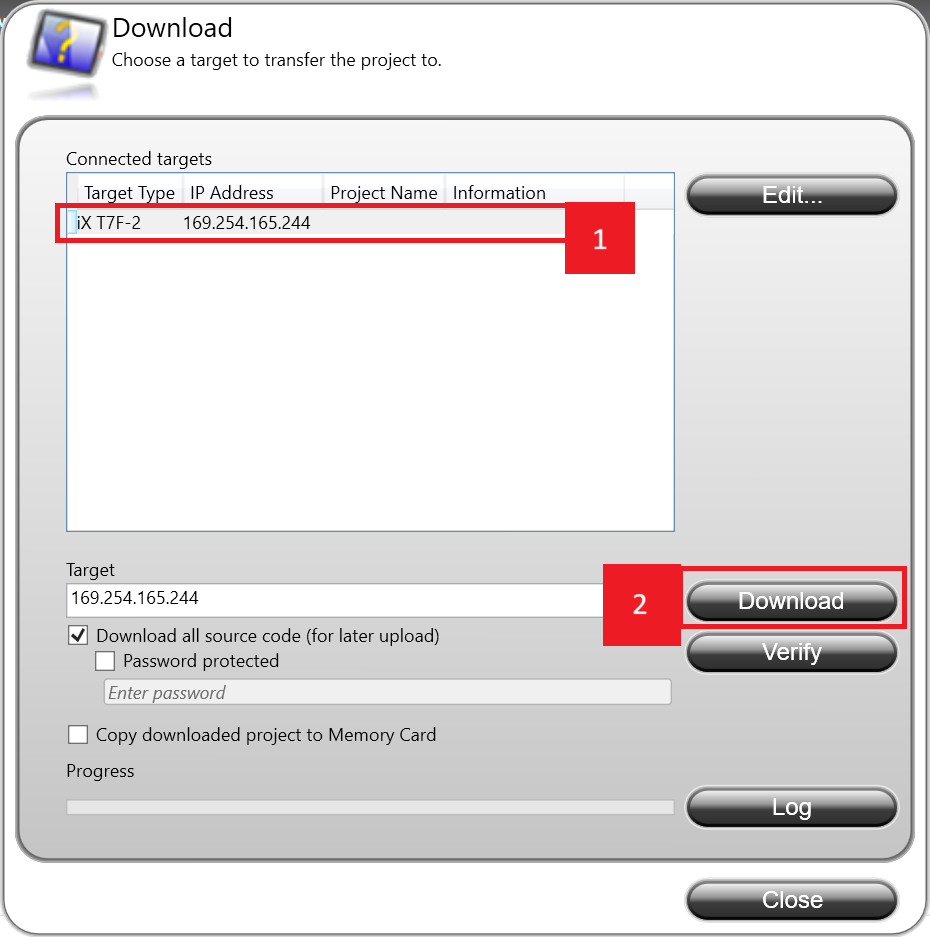
\includegraphics[width=10cm]
		{figuras/ix-project_download_ip-n}
		}}{ \Fonte{Elaborado pelo autor}    }
\end{figure}



Ao iniciar a transferência, 
o dispositivo entra em modo recepção, 
exibindo uma barra de progresso e 
mensagens de inicialização ao final do processo. 
Pode-se então fechar a janela clicando no botão 
\textbf{\textit{Close}}.

Projeto transferido ao Terminal Gráfico/IHM. 

O processo de compilação deve ser executado sempre que houver algum incremento ou ajuste no projeto, verificando assim, se não foi inserido algum erro ou falha no projeto.



	\chapter{Considerações finais e Contato}
\label{chap:conclusoes-e-trabalhos-futuros}

O presente trabalho buscou orientar de forma objetiva 
a construção da conexão entre uma 
IHM (Altus iX-T7F-2) e um CLP (Altus TB131), 
através de um protocolo de comunicação (Modbus), 
de modo a servir de contato inicial para 
a elaboração de propostas mais sofisticadas e 
atividades ou projetos mais interessantes de serem explorados, 
estudados e avaliados. 




\section{Contato}
\label{sec:contato}

A contribuição para 
a melhoria de metodologias educacionais e dos conteúdos técnicos, 
a correção de erros são sempre bem vindas. 

Para reportar erros a serem corrigidos ou 
propostas de melhorias a serem avaliadas, 
acesse o projeto deste documento em:

\textbf{\textit{{https://codeberg.org/JoseWRPereira/IX\_T7F\_2-operator\_panel}}} 

e reporte em \textbf{\textit{issues}}. 



Agradeço a colaboração!




	%\chapter{Como fazer?}
\label{cap:como_fazer}



\section{Motivação}
\label{sec:motivacao}


\section{Objetivos}
\label{sec:objetivos}



\subsection{Objetivo Geral}
\label{sec:objetivo-geral}


\subsection{Objetivos Específicos}
\label{sec:objetivos-especificos}



	\begin{alineas}
		\item Primeira
		\item Segunda
		\item Terceira
	\end{alineas}


\section{Figura}
\label{sec:figura}
	
	\begin{figure}[h!]
		\centering
		\Caption{\label{fig:exemplo-1} Lorem ipsum dolor sit amet, consectetur adipiscing elit. Suspendisse commodo lectus et augue elementum varius.}	
		\UECEfig{}{
			\fbox{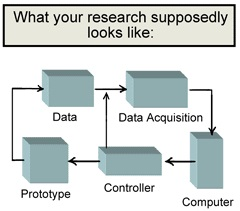
\includegraphics[width=8cm]{figuras/figura-1}}
		}{
			\Fonte{Elaborado pelo autor}
		}	
	\end{figure}


\section{Tabela}
\label{sec:tabela}

	\begin{table}[h!]	
	\centering
	\Caption{\label{tab:exemplo-1} Duis faucibus, enim quis tincidunt pellentesque, nisl leo varius nulla, vitae tempus dui mauris ac ante purus lorem}		
	\UECEtab{}{
		\begin{tabular}{cll}
			\toprule
			Ranking & Exon Coverage & Splice Site Support \\
			\midrule \midrule
			E1 & Complete coverage by a single transcript & Both splice sites\\
			E2 & Complete coverage by more than a single transcript & Both splice sites\\
			E3 & Partial coverage & Both splice sites\\
			E4 & Partial coverage & One splice site\\
			E5 & Complete or partial coverage & No splice sites\\
			E6 & No coverage & No splice sites\\
			\bottomrule
		\end{tabular}
	}{
		\Fonte{Elaborado pelo autor}
	}
	\end{table}


\section{alineascompont}
\label{sec:alineascompont}


\acrlong{DATASUS},

\acrlong{DNV},

\acrlong{DO},


\begin{alineascomponto}
	\item Primeira
	\item Segunda
	\item Terceira
	\begin{subalineascomponto}
		\item Primeira
		\item Segunda
	\end{subalineascomponto}
\end{alineascomponto}




O autor \cite{lamport1986latex} e \cite{Maia2011} e \cite{ibge23} \lipsum[2] 

\begin{table}[h!]
	\Caption{\label{tabela-ibge} Um Exemplo de tabela alinhada que pode ser longa ou curta, conforme padrão IBGE. conforme padrão IBGE. conforme padrão IBGE. conforme padrão IBGE. conforme padrão IBGE. conforme padrão IBGE. conforme padrão IBGE. conforme padrão IBGE. conforme padrão IBGE. conforme padrão IBGE. conforme padrão IBGE.}%
	\IBGEtab{}{%
		\begin{tabular}{ccc}
			\toprule
			Nome & Nascimento & Documento \\
			\midrule \midrule
			Maria da Silva & 11/11/1111 & 111.111.111-11 \\
			Maria da Silva & 11/11/1111 & 111.111.111-11 \\
			Maria da Silva & 11/11/1111 & 111.111.111-11 \\
			\bottomrule
		\end{tabular}%
	}{%
		\Fonte{Produzido pelos autores}%
		\Nota{Esta éuma nota, que diz que os dados são baseados na
			regressão linear.}%
		\Nota[Anotações]{Uma anotação adicional, seguida de várias outras.}%
	}
\end{table}

\cite{Huetal2000} 

\section{Exemplo de Algoritmos e Figuras}
\label{sec:exemplo-de-algoritmos-e-figuras}



\begin{algorithm}[h!]
	\SetSpacedAlgorithm
	\caption{\label{exemplo-de-algoritmo}Como escrever algoritmos no \LaTeX2e}
	\Entrada{o proprio texto}
	\Saida{como escrever algoritmos com \LaTeX2e }
	\Inicio{
		inicializa\c{c}\~ao\;
		\Repita{fim do texto}{
			leia o atual\;
			\Se{entendeu}{
				vá para o próximo\;
				próximo se torna o atual\;}
			\Senao{volte ao início da seção\;}
		}
	}	
\end{algorithm}







Exemplo de alíneas com números:

\begin{alineascomnumero}
	\item Primeira
	\item Segunda
\end{alineascomnumero}


\begin{table}[h!]	
	\centering
	\Caption{\label{tab:internal}Internal exon scores}	
	\IBGEtab{}{
		\begin{tabular}{cll}
			\toprule
			Ranking & Exon Coverage & Splice Site Support\\
			\midrule \midrule
			E1 & Complete coverage by a single transcript & Both splice sites\\
			E2 & Complete coverage by more than a single transcript & Both splice sites\\
			E3 & Partial coverage & Both splice sites\\
			E4 & Partial coverage & One splice site\\
			E5 & Complete or partial coverage & No splice sites\\
			E6 & No coverage & No splice sites\\
			\bottomrule
		\end{tabular}
	}{
		\Fonte{os autores}
	}
\end{table}

Referenciando a \autoref{tab:internal} 

\index{figuras}Figuras podem ser criadas diretamente em LaTeX, como o exemplo da \ref{fig-grafico-1}.

\begin{figure}[h!]
	\centering
	\Caption{\label{fig-grafico-1}Produção anual das dissertações de mestrado e teses de doutorado entre os anos de 1990 e 2008}		
	\IBGEtab{}{
		\fbox{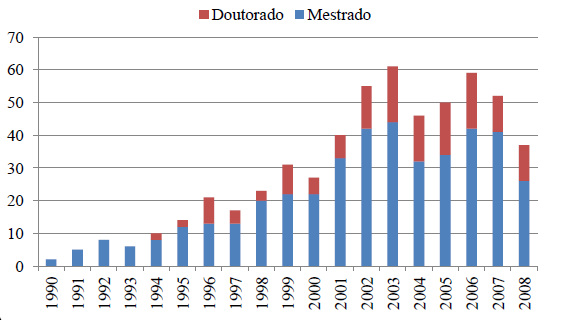
\includegraphics[scale=0.5]{figuras/figura-3}}
	}{
		\Fonte{os autores}
	}
\end{figure}

Ou então figuras podem ser incorporadas de arquivos externos, como é o caso da \autoref{fig-grafico-1}.  para manter a coerência no uso de software livre (já que você está usando LaTeX e abnTeX),  teste a ferramenta InkScape\index{InkScape}. ao CorelDraw\index{CorelDraw} ou ao Adobe Illustrator\index{Adobe! Illustrator}, \index{Gimp}Gimp. Ele é uma alternativa livre ao Adobe Photoshop\index{Adobe! Photoshop}.

\section{Usando Fórmulas Matemáticas}



\begin{equation}
	\begin{aligned}
		x = a_0 + \cfrac{1}{a_1
			+ \cfrac{1}{a_2
				+ \cfrac{1}{a_3 + \cfrac{1}{a_4} } } }
	\end{aligned}
\end{equation}


\begin{equation}
	\begin{aligned}
		k_{n+1} = n^2 + k_n^2 - k_{n-1}
	\end{aligned}
\end{equation}


\begin{equation}
	\begin{aligned}
		\cos (2\theta) = \cos^2 \theta - \sin^2 \theta
	\end{aligned}
\end{equation}


\begin{equation}
	\begin{aligned}
		A_{m,n} =
		\begin{pmatrix}
			a_{1,1} & a_{1,2} & \cdots & a_{1,n} \\
			a_{2,1} & a_{2,2} & \cdots & a_{2,n} \\
			\vdots  & \vdots  & \ddots & \vdots  \\
			a_{m,1} & a_{m,2} & \cdots & a_{m,n}
		\end{pmatrix}
	\end{aligned}
\end{equation}


\begin{equation}
	\begin{aligned}
		f(n) = \left\{ 
		\begin{array}{l l}
			n/2 & \quad \text{if $n$ is even}\\
			-(n+1)/2 & \quad \text{if $n$ is odd}
		\end{array} \right.
	\end{aligned}
\end{equation}






\section{Usando Algoritmos}


\begin{algorithm}[h!]
	\SetSpacedAlgorithm
	\caption{\label{alg:algoritmo_de_colonica_de_formigas}Algoritmo de Otimização por Colônia de Formiga}
	\Entrada{Entrada do Algoritmo}
	\Saida{Saida do Algoritmo}
	\Inicio{
		Atribua os valores dos parâmetros\;
		Inicialize as trilhas de feromônios\;
		\Enqto{não atingir o critério de parada}{
			\Para{cada formiga}{
				Construa as Soluções\;
			}
			Aplique Busca Local (Opcional)\;
			Atualize o Feromônio\;
		}	
	}		
\end{algorithm}


\section{Usando Código-fonte}


\lstinputlisting[language=C++,caption={Hello World em C++}]{figuras/main.cpp}


\begin{lstlisting}[language=Java,caption={Hello World em Java}]
	public class HelloWorld {
		public static void main(String[] args) {
			System.out.println("Hello World!");
		}
	}
\end{lstlisting}


\section{Usando Teoremas, Proposições, etc}


\begin{teo}[Pitágoras]
	Em todo triângulo retângulo o quadrado do comprimento da
	hipotenusa é igual a soma dos quadrados dos comprimentos dos catetos.
\end{teo}



\begin{teo}[Fermat]
	Não existem inteiros $n > 2$, e $x, y, z$ tais que $x^n + y^n = z$
\end{teo}


\begin{prop}
	Para demonstrar o Teorema de Pitágoras...
\end{prop}


\begin{exem}
	Este é um exemplo do uso do ambiente exe definido acima.
\end{exem}


\begin{xdefinicao}
	Definimos o produto de ...
\end{xdefinicao}


\section{Usando Questões}



\begin{questao}
	\item Esta é a primeira questão com alguns itens:
	\begin{enumerate}
		\item Este é o primeiro item
		\item Segundo item
	\end{enumerate}
	\item Esta é a segunda questão:
	\begin{enumerate}
		\item Este é o primeiro item
		\item Segundo item
	\end{enumerate}
	\item Lorem ipsum dolor sit amet, consectetur adipiscing elit. Nunc dictum sed tortor nec viverra. consectetur adipiscing elit. Nunc dictum sed tortor nec viverra.
	\begin{enumerate}
		\item consectetur
		\item adipiscing
		\item Nunc
		\item dictum
	\end{enumerate}
\end{questao}

\section{Citações}

\subsection{Documentos com três autores}

Quando houver três autores na citação, apresentam se os três, separados por ponto e vírgula, caso estes estejam após o texto. Se os autores estiverem incluídos no texto, devem ser separados por vírgula e pela conjunção "e".

\citeautoronline{tresautores}

\cite{tresautores}

\subsection{Documentos com mais de três autores}
Havendo mais de três autores, indica-se o primeiro seguido da expressão \textit{et al.} (do latim \textit{et alli}, que significa e outros), do ano e da página.

\citeautoronline{quatroautores}

\cite{quatroautores}

\subsection{Documentos de vários autores}

Havendo    citações    indiretas de    diversos    documentos    de    vários    autores, mencionados  simultaneamente e  que  expressam  a  mesma  ideia,  separam-se  os  autores  por ponto e vírgula, em ordem alfabética.

\cite{tresautores, quatroautores}

\section{Notas de Rodap\'{e}}

Deve-se utilizar o sistema autor-data para as  citações no texto e o numérico para notas explicativas\footnote{Veja - se como exemplo desse tipo de abordagem o estudo de Netzer (1976)}. As notas de rodapé podem e devem ser alinhadas, a partir da segunda linha da mesma nota, abaixo da primeira letra da primeira palavra, de forma a destacar o expoente \footnote{Encontramos  esse  tipo  de  perspectiva  na  2ª  parte  do  verbete  referido  na  nota  anterior,  em  grande  parte  do estudo de Rahner (1962).} e sem espaço entre elas e com fonte menor (tamanho 10).

	
	%Elementos pós-textuais	
	\bibliography{elementos-pos-textuais/referencias}
	%\imprimirglossario	
	%\imprimirapendices
		% Adicione aqui os apendices do seu trabalho
%		\apendice{Lorem Ipsum}
\label{ap:lorem-ipsum}

\lipsum[1]
%		\apendice{Modelo de Capa}
\label{ap:modelo-de-capa}

\lipsum[1]

%		\apendice{Termo de Fiel Depositário}
\label{ap:termo-de-fiel-depositario}

\noindent \textbf{Pesquisa:} ANÁLISE DA MORTALIDADE INFANTIL COM MALFORMAÇÕES CONGÊNITAS.

\noindent Pelo presente instrumento que atende às exigências legais, a Sra. Maria Consuelo Martins Saraiva, ``fiel depositário'' com o cargo de Secretária Municipal de Saúde de Iracema, após ter tomado conhecimento do protocolo de pesquisa intitulado: ANÁLISE DA MORTALIDADE INFANTIL COM MALFORMAÇÕES CONGÊNITAS. Analisando a repercussão desse estudo no contexto da saúde pública e epidemiologia, autoriza Karla Maria da Silva Lima, enfermeira, aluna do Curso de Mestrado Acadêmico em Enfermagem da Universidade Estadual do Ceará (UECE), sob orientação do Prof. Dr. José Maria de Castro, da UECE, ter acesso aos bancos de dados do Sistema de Informação sobre Nascidos Vivos e do Sistema de Informação sobre Mortalidade da Secretaria Municipal de Saúde de Iracema, objeto deste estudo, e que se encontram sob sua total responsabilidade. Fica claro que o Fiel Depositário pode a qualquer momento retirar sua AUTORIZAÇÃO e ciente de que todas as informações prestadas tornar-se-ão confidenciais e guardadas por força de sigilo profissional, assegurando que os dados obtidos da pesquisa serão somente utilizados para estudo.	
	%\imprimiranexos
		% Adicione aqui os anexos do seu trabalho
%		\anexo{Exemplo de Anexo}
\label{an:exemplo-de-anexo}

\lipsum[13]		
%		\anexo{Dinâmica das classes sociais}
\label{an:dinamica-das-classes-sociais}

\lipsum[14]
\index{AAA}
	%\imprimirindice

\end{document}
